%% LyX 2.1.3 created this file.  For more info, see http://www.lyx.org/.
%% Do not edit unless you really know what you are doing.
\RequirePackage{fix-cm}
\documentclass[8pt]{extbook}
\usepackage{bera}
\usepackage[T1]{fontenc}
\usepackage[utf8]{inputenc}
\usepackage[a5paper]{geometry}
\geometry{verbose,tmargin=1.9cm,bmargin=1.9cm,lmargin=1.9cm,rmargin=1.2cm}
\usepackage{fancyhdr}
\pagestyle{fancy}
\setcounter{secnumdepth}{0}
\setcounter{tocdepth}{3}
\usepackage{array}
\usepackage{longtable}
\usepackage{booktabs}
\usepackage{calc}
\usepackage{textcomp}
\usepackage{url}
\usepackage{pdfpages}
\usepackage{fixltx2e}
\usepackage{makeidx}
\makeindex
\usepackage{graphicx}
\usepackage[unicode=true,
 bookmarks=true,bookmarksnumbered=false,bookmarksopen=false,
 breaklinks=false,pdfborder={0 0 1},backref=false,colorlinks=false]
 {hyperref}
\hypersetup{pdftitle={EMNLP 2015 Handbook},
 pdfauthor={Fernando Batista},
 pdfsubject={EMNLP 2015},
 pdfkeywords={EMNLP 2015, Handbook},
 colorlinks, citecolor=dkblue, filecolor=dkblue, linkcolor=dkblue, urlcolor=blue}

\makeatletter

%%%%%%%%%%%%%%%%%%%%%%%%%%%%%% LyX specific LaTeX commands.
%% Because html converters don't know tabularnewline
\providecommand{\tabularnewline}{\\}
%% A simple dot to overcome graphicx limitations
\newcommand{\lyxdot}{.}


%%%%%%%%%%%%%%%%%%%%%%%%%%%%%% Textclass specific LaTeX commands.
\usepackage{enumitem}		% customizable list environments
\newlength{\lyxlabelwidth}      % auxiliary length 

%%%%%%%%%%%%%%%%%%%%%%%%%%%%%% User specified LaTeX commands.
\usepackage{biblatex}

\usepackage{handbook}
\usepackage{emnlp2015}

\usepackage[Bjornstrup]{fncychap}

\usepackage{color}
\definecolor{mygray}{gray}{0.75}
\definecolor{dkblue}{rgb}{0,0,0.4}

\usepackage{marginnote}
\usepackage{graphicx}
\usepackage{ragged2e}
\usepackage{multirow}

\addbibresource{/Users/fmmb/Dropbox/Events/EMNLP2015/handbook/content/tutorials.bib}
\addbibresource{/Users/fmmb/Dropbox/Events/EMNLP2015/handbook/content/workshops.bib}

\addbibresource{/Users/fmmb/Dropbox/Events/EMNLP2015/handbook/auto/papers/papers.bib}
\addbibresource{/Users/fmmb/Dropbox/Events/EMNLP2015/handbook/auto/tacl-final/papers.bib}

\addbibresource{/Users/fmmb/Dropbox/Events/EMNLP2015/handbook/auto/CogACLL/papers.bib}
\addbibresource{/Users/fmmb/Dropbox/Events/EMNLP2015/handbook/auto/DiscoMT15/papers.bib}
\addbibresource{/Users/fmmb/Dropbox/Events/EMNLP2015/handbook/auto/LSDSem/papers.bib}
\addbibresource{/Users/fmmb/Dropbox/Events/EMNLP2015/handbook/auto/Louhi15/papers.bib}
\addbibresource{/Users/fmmb/Dropbox/Events/EMNLP2015/handbook/auto/VL15/papers.bib}
\addbibresource{/Users/fmmb/Dropbox/Events/EMNLP2015/handbook/auto/WASSA15/papers.bib}
\addbibresource{/Users/fmmb/Dropbox/Events/EMNLP2015/handbook/auto/WMT15/papers.bib}

\makeatother

\begin{document}
\pagestyle{empty}

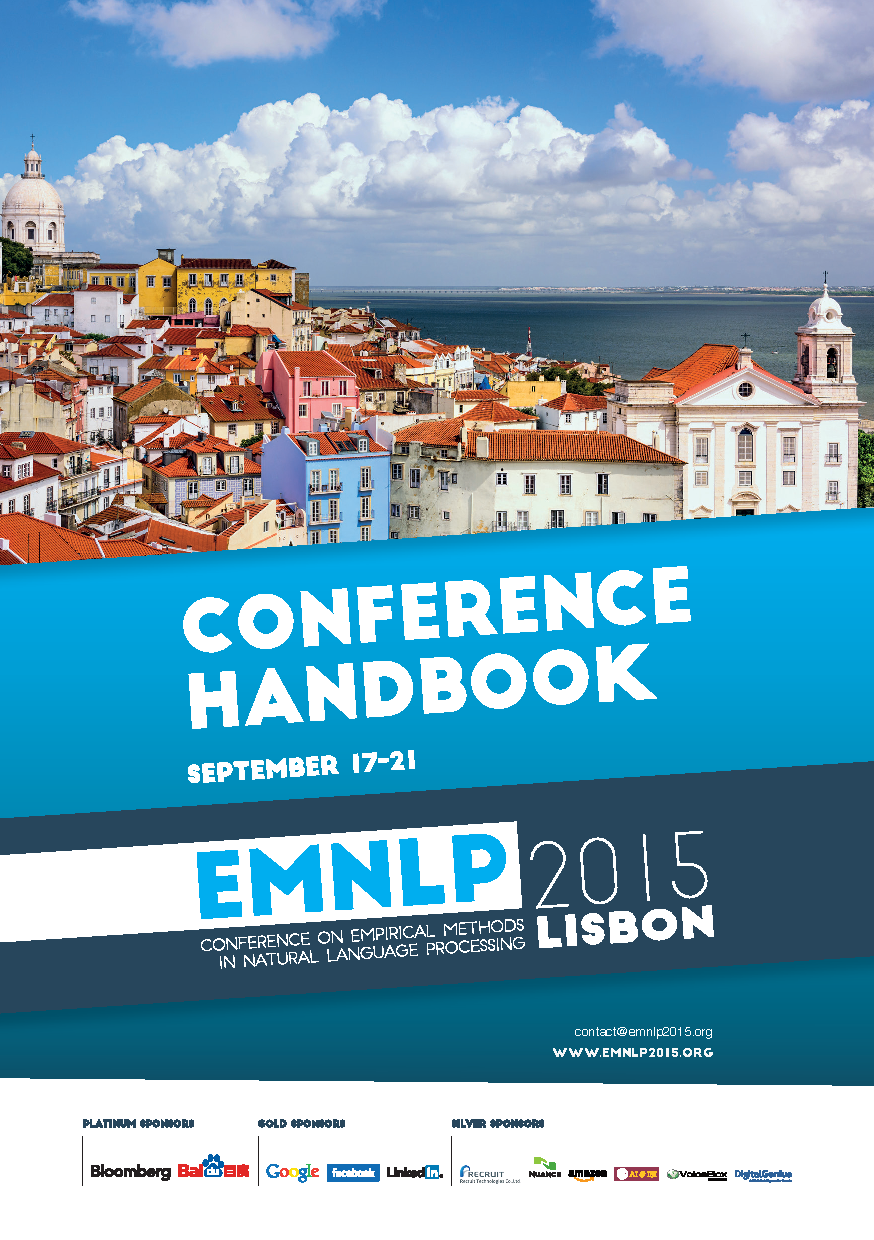
\includepdf{content/images/frontcover}

\vspace*{-1.2cm}
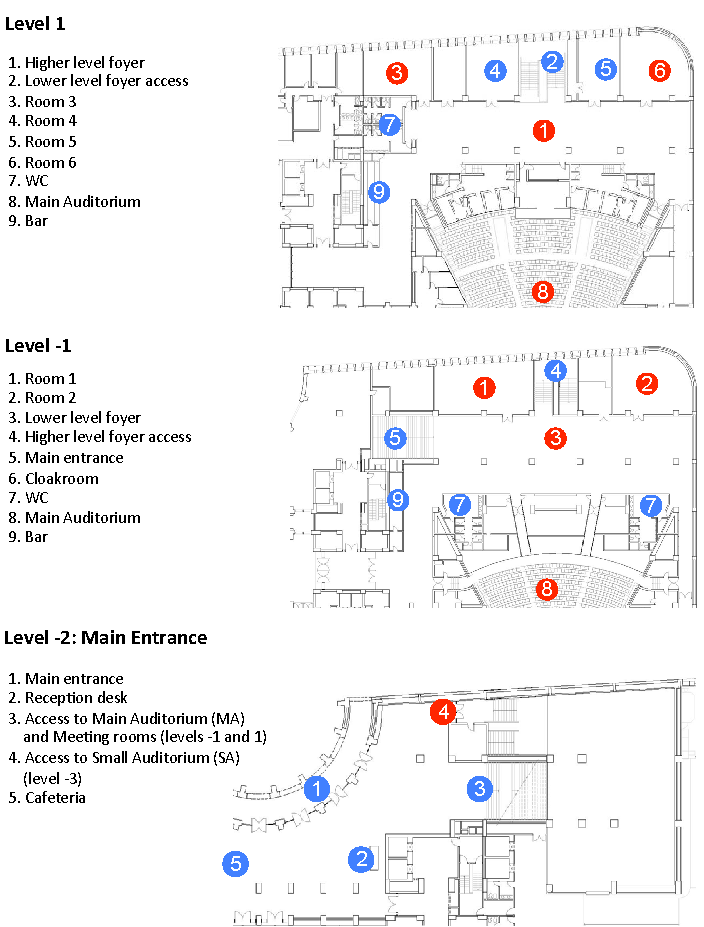
\includegraphics[width=1\columnwidth]{content/images/culturgest-maps}

\vfill{}


\emph{Cover design by Sarah Almeida}

\emph{Thanks to Matt Post for his helpful notes about creating a handbook}

\emph{Handbook assembled by Fernando Batista}

\cleardoublepage{}

\pagestyle{fancy}
\pagenumbering{gobble}

\markright{Schedule at a Glance (Overall)}

\begin{center}
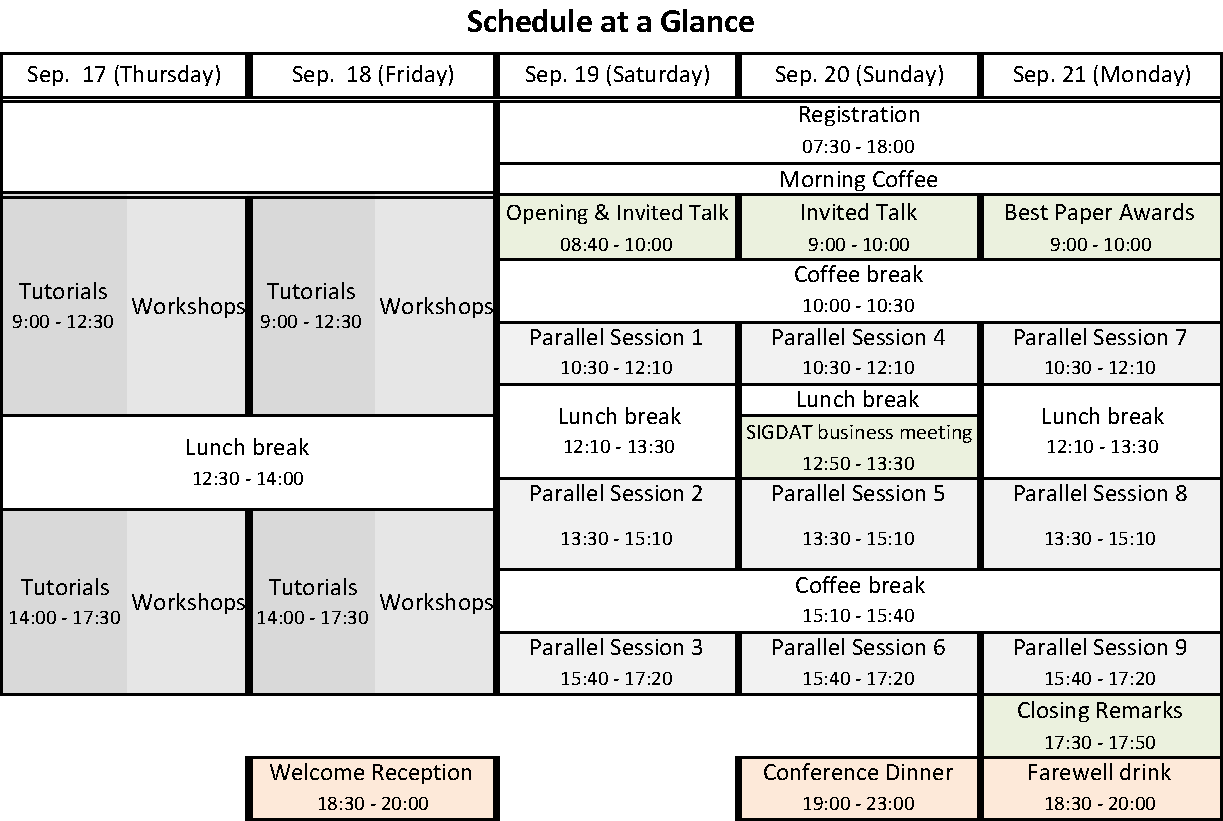
\includegraphics[angle=90,height=0.97\textheight]{content/images/schedule-at-glance}
\par\end{center}

\clearpage{}

\markright{Schedule Overview}

\small

\vspace*{-4ex}


\noindent \textbf{Thursday, September 17}

\vspace{-1.7ex}


\noindent \rule{1\columnwidth}{1pt}

\vspace{-4ex}


\renewcommand{\arraystretch}{1.2}
\begin{SingleTrackSchedule}
  09:00 & -- & 17:30 & {\bfseries Tutorials}\\
  09:00 & -- & 19:30 & {\bfseries Workshops}\\
\end{SingleTrackSchedule}

\vspace*{-2ex}


\noindent \textbf{Friday, September 18}

\vspace{-1.7ex}


\noindent \rule{1\columnwidth}{1pt}

\vspace{-4ex}


\renewcommand{\arraystretch}{1.2}
\begin{SingleTrackSchedule}
  09:00 & -- & 17:30 & {\bfseries Tutorials}\\
  09:00 & -- & 18:00 & {\bfseries Workshops}\\
  18:30 & -- & 20:00 & {\bfseries Welcome Reception} \hfill \emph{\WelcomeLoc}\\
\end{SingleTrackSchedule}

\vspace*{-2ex}


\noindent \textbf{Saturday, September 19}

\vspace{-1.7ex}


\noindent \rule{1\columnwidth}{1pt}

\vspace{-4ex}


\renewcommand{\arraystretch}{1.2}
\begin{SingleTrackSchedule}
  07:30 & -- & 18:00 &
  {\bfseries Registration} \hfill \emph{\RegistrationLoc}
  \\
  08:40 & -- & 10:00 &
  {\bfseries Session P1: Plenary Session} \hfill \emph{Main Auditorium}
  \\
 08:40 & -- & 09:00 & \textit{Opening Remarks and Introductory Speeches (General Chair, Program Co-Chairs and Local Co-Chairs)}\\
 09:00 & -- & 10:00 & \textit{Invited Talk: Deep Learning of Semantic Representations (Yoshua Bengio)}\\
  10:00 & -- & 10:30 &
  {\bfseries Coffee break} \hfill \emph{\CoffeeLoc}
  \\
  10:30 & -- & 12:10 &
  {\bfseries Session 1}\\

 & \multicolumn{3}{l}{%
 \begin{minipage}[t]{0.94\linewidth}
  \begin{tabular}{|>{\RaggedRight}p{0.235\linewidth}|>{\RaggedRight}p{0.235\linewidth}|>{\RaggedRight}p{0.235\linewidth}|>{\RaggedRight}p{0.235\linewidth}|}
  \hline
Semantics (Long + TACL Papers) & Machine Translation (Long + TACL Papers) & NLP for Web and Social Media, including Computational Social Science (Long Papers) & Long Paper Posters \rule{1\linewidth}{0.1pt} Short Paper Posters \\
\emph{\TrackALoc} & \emph{\TrackBLoc} & \emph{\TrackCLoc} & \emph{\TrackDLoc} \\
  \hline\end{tabular}
\end{minipage}
}\\
  12:10 & -- & 13:30 &
  {\bfseries Lunch} \hfill \emph{\LunchLoc}
  \\
  13:30 & -- & 15:10 &
  {\bfseries Session 2}\\

 & \multicolumn{3}{l}{%
 \begin{minipage}[t]{0.94\linewidth}
  \begin{tabular}{|>{\RaggedRight}p{0.235\linewidth}|>{\RaggedRight}p{0.235\linewidth}|>{\RaggedRight}p{0.235\linewidth}|>{\RaggedRight}p{0.235\linewidth}|}
  \hline
Statistical Models and Machine Learning Methods (Long + TACL Papers) & Tagging, Chunking and Parsing (Long +TACL Papers) & Summarization (Long Papers) & Long Paper Posters \rule{1\linewidth}{0.1pt} Short Paper Posters \\
\emph{\TrackALoc} & \emph{\TrackBLoc} & \emph{\TrackCLoc} & \emph{\TrackDLoc} \\
  \hline\end{tabular}
\end{minipage}
}\\
  15:10 & -- & 15:40 &
  {\bfseries Coffee break} \hfill \emph{\CoffeeLoc}
  \\
  15:40 & -- & 17:20 &
  {\bfseries Session 3}\\

 & \multicolumn{3}{l}{%
 \begin{minipage}[t]{0.94\linewidth}
  \begin{tabular}{|>{\RaggedRight}p{0.235\linewidth}|>{\RaggedRight}p{0.235\linewidth}|>{\RaggedRight}p{0.235\linewidth}|>{\RaggedRight}p{0.235\linewidth}|}
  \hline
Sentiment Analysis and Opinion Mining (Long Papers) & Semantics (Long +TACL Papers) & Information Retrieval and Question Answering (Long Papers) & Long + TACL Paper Posters \rule{1\linewidth}{0.1pt} Short Paper Posters \\
\emph{\TrackALoc} & \emph{\TrackBLoc} & \emph{\TrackCLoc} & \emph{\TrackDLoc} \\
  \hline\end{tabular}
\end{minipage}
}\\
\end{SingleTrackSchedule}


\vspace*{-2ex}


\noindent \textbf{Sunday, September 20}

\vspace{-1.7ex}


\noindent \rule{1\columnwidth}{1pt}

\vspace{-4ex}


\renewcommand{\arraystretch}{1.2}
\begin{SingleTrackSchedule}
  07:30 & -- & 18:00 &
  {\bfseries Registration} \hfill \emph{\RegistrationLoc}
  \\
  08:00 & -- & 09:00 &
  {\bfseries Morning Coffee} \hfill \emph{\MorningLoc}
  \\
  09:00 & -- & 10:00 &
  {\bfseries Session P2: Plenary Session} \hfill \emph{Main Auditorium}
  \\
 & & & \textit{Invited Talk: Measuring How Elected Officials and Constituents Communicate (Justin Grimmer)}\\
  10:00 & -- & 10:30 &
  {\bfseries Coffee break} \hfill \emph{\CoffeeLoc}
  \\
  10:30 & -- & 12:10 &
  {\bfseries Session 4}\\

 & \multicolumn{3}{l}{%
 \begin{minipage}[t]{0.94\linewidth}
  \begin{tabular}{|>{\RaggedRight}p{0.235\linewidth}|>{\RaggedRight}p{0.235\linewidth}|>{\RaggedRight}p{0.235\linewidth}|>{\RaggedRight}p{0.235\linewidth}|}
  \hline
Information Extraction (Long Papers) & Statistical Models and Machine Learning Methods (Long Papers) & Discourse (Long +TACL Papers) & Long Paper Posters \rule{1\linewidth}{0.1pt} Short Paper Posters \\
\emph{\TrackALoc} & \emph{\TrackBLoc} & \emph{\TrackCLoc} & \emph{\TrackDLoc} \\
  \hline\end{tabular}
\end{minipage}
}\\
  12:10 & -- & 12:50 &
  {\bfseries Lunch} \hfill \emph{\LunchLoc}
  \\
  12:50 & -- & 13:30 &
  {\bfseries Session P3: SIGDAT business meeting} \hfill \emph{Main Auditorium}
  \\
  13:30 & -- & 15:10 &
  {\bfseries Session 5}\\

 & \multicolumn{3}{l}{%
 \begin{minipage}[t]{0.94\linewidth}
  \begin{tabular}{|>{\RaggedRight}p{0.235\linewidth}|>{\RaggedRight}p{0.235\linewidth}|>{\RaggedRight}p{0.235\linewidth}|>{\RaggedRight}p{0.235\linewidth}|}
  \hline
Text Mining and NLP Applications (Long + TACL Papers) & Semantics (Long +TACL Papers) & Phonology and Word Segmentation (Long Papers) & Long Paper Posters \rule{1\linewidth}{0.1pt} Short Paper Posters \\
\emph{\TrackALoc} & \emph{\TrackBLoc} & \emph{\TrackCLoc} & \emph{\TrackDLoc} \\
  \hline\end{tabular}
\end{minipage}
}\\
  15:10 & -- & 15:40 &
  {\bfseries Coffee break} \hfill \emph{\CoffeeLoc}
  \\
  15:40 & -- & 17:20 &
  {\bfseries Session 6}\\

 & \multicolumn{3}{l}{%
 \begin{minipage}[t]{0.94\linewidth}
  \begin{tabular}{|>{\RaggedRight}p{0.235\linewidth}|>{\RaggedRight}p{0.235\linewidth}|>{\RaggedRight}p{0.235\linewidth}|>{\RaggedRight}p{0.235\linewidth}|}
  \hline
Machine Translation (Long Papers) & Sentiment Analysis and Opinion Mining / Tagging, Chunking and Parsing (Long Papers) & Language and Vision / Information Extraction (Long Papers) & Long Paper Posters \rule{1\linewidth}{0.1pt} Short Paper Posters \\
\emph{\TrackALoc} & \emph{\TrackBLoc} & \emph{\TrackCLoc} & \emph{\TrackDLoc} \\
  \hline\end{tabular}
\end{minipage}
}\\
  19:00 & -- & 23:00 &
  {\bfseries Conference Dinner} \hfill \emph{Pateo Alfacinha}
  \\
\end{SingleTrackSchedule}


\vspace*{-2ex}


\noindent \textbf{Monday, September 21}

\vspace{-1.7ex}


\noindent \rule{1\columnwidth}{1pt}

\vspace{-4ex}


\renewcommand{\arraystretch}{1.2}
\begin{SingleTrackSchedule}
  07:30 & -- & 18:00 &
  {\bfseries Registration} \hfill \emph{\RegistrationLoc}
  \\
  08:00 & -- & 09:00 &
  {\bfseries Morning Coffee} \hfill \emph{\MorningLoc}
  \\
  09:00 & -- & 10:00 &
  {\bfseries Session P4: Plenary Session} \hfill \emph{Main Auditorium}
  \\
 09:00 & -- & 09:05 & \textit{Best Paper Awards (Chris Callison-Burch and Jian Su)}\\
 09:05 & -- & 09:30 & \paperlistentry{papers-662}\\
 09:30 & -- & 09:55 & \paperlistentry{papers-072}\\
 09:55 & -- & 10:05 & \paperlistentry{papers-536}\\
  10:05 & -- & 10:30 &
  {\bfseries Coffee break} \hfill \emph{\CoffeeLoc}
  \\
  10:30 & -- & 12:10 &
  {\bfseries Session 7}\\

 & \multicolumn{3}{l}{%
 \begin{minipage}[t]{0.94\linewidth}
  \begin{tabular}{|>{\RaggedRight}p{0.235\linewidth}|>{\RaggedRight}p{0.235\linewidth}|>{\RaggedRight}p{0.235\linewidth}|>{\RaggedRight}p{0.235\linewidth}|}
  \hline
Semantics (Long +TACL Papers) & Information Extraction (Long Papers) & Computational Psycholinguistics / Machine Translation (Long Papers) & Long +TACL Paper Posters \rule{1\linewidth}{0.1pt} Short Paper Posters \\
\emph{\TrackALoc} & \emph{\TrackBLoc} & \emph{\TrackCLoc} & \emph{\TrackDLoc} \\
  \hline\end{tabular}
\end{minipage}
}\\
  12:10 & -- & 13:30 &
  {\bfseries Lunch} \hfill \emph{\LunchLoc}
  \\
  13:30 & -- & 15:15 &
  {\bfseries Session 8}\\

 & \multicolumn{3}{l}{%
 \begin{minipage}[t]{0.94\linewidth}
  \begin{tabular}{|>{\RaggedRight}p{0.235\linewidth}|>{\RaggedRight}p{0.235\linewidth}|>{\RaggedRight}p{0.235\linewidth}|>{\RaggedRight}p{0.235\linewidth}|}
  \hline
Fun and Quirky Topics (Short Papers) & Semantics (Short Papers) & Statistical Models and Machine Learning Methods / Machine Translation (Short Papers) & Long Paper Posters \rule{1\linewidth}{0.1pt} Short Paper Posters \\
\emph{\TrackALoc} & \emph{\TrackBLoc} & \emph{\TrackCLoc} & \emph{\TrackDLoc} \\
  \hline\end{tabular}
\end{minipage}
}\\
  15:15 & -- & 15:40 &
  {\bfseries Coffee break} \hfill \emph{\CoffeeLoc}
  \\
  15:40 & -- & 17:20 &
  {\bfseries Session 9}\\

 & \multicolumn{3}{l}{%
 \begin{minipage}[t]{0.94\linewidth}
  \begin{tabular}{|>{\RaggedRight}p{0.235\linewidth}|>{\RaggedRight}p{0.235\linewidth}|>{\RaggedRight}p{0.235\linewidth}|>{\RaggedRight}p{0.235\linewidth}|}
  \hline
Statistical Models and Machine Learning Methods (Long + TACL Papers) & Text Mining and NLP Applications (Long Papers) & Spoken Language Processing and Language Modeling (Long Papers) & Long Paper Posters \rule{1\linewidth}{0.1pt} Short Paper Posters \\
\emph{\TrackALoc} & \emph{\TrackBLoc} & \emph{\TrackCLoc} & \emph{\TrackDLoc} \\
  \hline\end{tabular}
\end{minipage}
}\\
  17:30 & -- & 17:50 &
  {\bfseries Session P5: Closing Remarks} \hfill \emph{Main Auditorium}
  \\
  18:30 & -- & 20:00 &
  {\bfseries Farewell Drink} \hfill \emph{Culturgest}
  \\
\end{SingleTrackSchedule}


\normalsize

\clearpage{}

\markright{Quick information}


\section*{WIFI access}

\textbf{Username}: EMNLP2015

\textbf{Password}: Lisboa2015


\section*{Links}

Web site: \url{www.emnlp2015.org}

Contact email: \url{contact@emnlp2015.org}

Find us on facebook: \url{https://www.facebook.com/emnlp2015}

Follow us on twitter: \url{https://twitter.com/emnlp2015}

Discussion group: \url{https://groups.google.com/forum/?hl=en#!forum/emnlp-2015}

Conference4me app: \url{http://conference4me.psnc.pl/download/}

\clearpage{}\thispagestyle{empty}


\cleardoublepage{}

\frontmatter

\pagestyle{plain}



\tableofcontents{}

\mainmatter

\pagestyle{fancy}


\chapter{Conference Information}


\section{Preface by the General Chair}

\begin{flushright}
August 25, 2015 
\par\end{flushright}

\noindent Welcome to the 2015 Conference on Empirical Methods in Natural
Language Processing. EMNLP is annually organized by SIGDAT, the Association
for Computational Linguistics' special interest group on linguistic
data and corpus-based approaches to NLP. This year the conference
will be held on September 17--21 in the enchanting city of Lisbon,
Portugal.\footnote{Conference website: \texttt{http://www.emnlp2015.org}}

EMNLP has continued to increase in prominence as one of the most important
conferences in Natural Language Processing (NLP). This year the conference
has experienced an unprecedented boost in submitted papers. I believe
that this reflects both the growth of the NLP field and also the health
and strength of the conference itself, with a history of many years
of solid work. With this level of interest at submission time, we
are also expecting a record attendance. The conference will span a
five-day period this year, and it requires a growing organization
structure.

Some of the features introduced in EMNLP 2014 will continue this year
(e.g., tutorials, new chairs, posters as parallel sessions, flat rates
and flexibility for tutorials and workshops, etc.). We also introduce
some innovations, like a revised selection process for which talks
are presented as talks versus posters.

This year I had the privilege of coordinating the conference from
my General Chair position. This has been a very instructive and enriching
exercise which showed me the conference as a whole, from many different
angles. Prefaces in the proceedings invariably praise the team of
organizers. This one will not be an exception. Organizing a large
conference as EMNLP requires excellent people working as a team in
multiple interrelated tasks. I have been lucky to work with an outstanding
team of people, from whom I learnt a lot. These aren't empty words.
I would like to thank each and every chair for the hard work that
made the conference a reality.

The Program Chairs, Jian Su and Chris Callison-Burch, did an excellent
job at putting together a very interesting program with over 300 papers.
They had to deal with a very large number of submissions, which exceeded
even our most optimistic expectations. As a consequence, they were
forced to be creative and to find solutions on the fly to adapt to
the situation. They recruited the largest ever program committee and
successfully managed a huge reviewing and decision making process
under a very tight schedule. A real gift for the general chair. They
complemented the program with very interesting keynote speakers, Yoshua
Bengio and Justin Grimmer who will present exciting research topics
for our community.

The EMNLP 2015 main conference is accompanied by 7 workshops and 8
tutorials during the first two days. The Workshops Chairs, Zornitsa
Kozareva and Jörg Tiedemann, and the Tutorials Chairs, Maggie Li and
Khalil Sima'an, conducted the selection processes in a joint effort
with the other ACL conferences in 2015 (NAACL and ACL-IJCNLP). This
has been the standard procedure from last years. It has the advantage
of starting early, avoiding duplicated reviewing and allowing a more
balanced selection among conferences. EMNLP attracted a varied and
interesting set of workshops and tutorials, which gives more value
to the conference.

Daniele Pighin and Yuval Marton were responsible for the always difficult
and sometimes thankless task of putting together the conference publications.
This is a very complex effort which involves coordination with almost
everyone in the team under the pressure of hard publication deadlines.
Yuval is serving in this position for a second year. Staggered two
year terms for publication chairs is a new addition for EMNLP starting
this year, and we hope that it will be a permanent feature. In the
first year, publication chairs will learn and do the bulk of proceedings
compilation. During the second year their role will be more advisory,
instructing and helping the first-year chair. This procedure will
help the transmission of the necessary know-how from year to year.
Thanks to Yuval and Daniele for accepting the challenge and making
it work wonderfully. Finally, this is the second year that EMNLP uses
a mobile app for the conference program (Conference4me). The publication
chairs also coordinated the integration of the app with SoftConf,
which is now smoother and more seamless.

The local organization team was led by André Martins and João Graça.
They did an amazing job, working hard and with all the complexities
and subtleties of local arrangements. One of the keys for the success
was the creation of a large team of local organizers with clearly
defined roles and responsibilities. They appointed very committed
people: Isabel Trancoso (Local Publicity Chair), Fernando Batista
(Handbook Chair), Bruno Martins (Website and App Chair), Luísa Coheur
(Student Volunteer Coordinator), and Helena Moniz (Local Arrangements
Chair). Thanks to all. I am especially pleased about the new website,
which was revamped and looks more professional everyday. This is certainly
a good investment for the future.

A large conference as EMNLP needs to focus on dissemination activities
too. Barbara Plank acted as the international Publicity Chair. She
did a fantastic job and coordinated very well with the local publicity
and the website chairs. The calls for papers, calls for participation,
and main news of the conference were timely distributed through ACL,
the usual distribution lists, and also through the conference website
and two Facebook and Twitter accounts. The EMNLP2015 Twitter account
garnered more followers than in previous years.

I am really grateful to SIGDAT. Its secretary, Noah Smith, acted as
the liasion between SIGDAT and the conference organizers. He was always
available and ready to help with very good advice. SIGDAT also provided
the funds for the student scholarship program. These grants help covering
traveling expenses to a dozen of students. The committee appointed
for collecting the applications and making the decisions was formed
by Francisco Guzmán and Llu\'{i}s Padró, who had to analyze all the
information and decide the awardees in only a few days.

Another sign of the health of EMNLP and the field in general is the
interest showed by sponsors. Thanks to the work of our sponsorship
team, formed by João Graça and Hang Li, in coordination with the ACL
International Sponsorship Committee, we got a record number of 13
sponsors for EMNLP 2015 (2 platinum, 3 gold, 6 silver and 2 bronze).
In addition to these direct sponsors, we also have several smaller
supporters, exhibitors, and institutional partners. We are extremely
grateful to all these companies and institutions, which make a better
conference possible at a more affordable registration fee.

Additionally, we counted on the invaluable help of Priscilla Rasmussen,
supporting the local organization in all fronts with her broad experience.
She took care of the registration process too. We also got very good
advice, know-how, and helpful software and forms from last year general
chair and local organizers, Alessandro Moschitti and Kareem Darwish.
Thank you.

Finally, I would like to thank the authors of submitted and accepted
papers, and all the attendees to the conference, who will be the main
actors from September 17 to September 21, 2015. I am convinced that
we will experience a fantastic conference, scientifically exciting
and full of fond memories, in the unique environment of Lisbon. 

\begin{flushright}
\emph{Lluís Màrquez}\index{Màrquez, Lluís}\\
 EMNLP 2015 General Chair 
\par\end{flushright}

\newpage{}


\section{Preface by the Program Committee Co-Chairs}

\begin{flushright}
August 25, 2015 
\par\end{flushright}

\noindent Welcome to the 2015 Conference on Empirical Methods in Natural
Language Processing! This year we received a record number of submissions.
There were 1300 valid submissions. The 600 long papers and 700 short
papers were allocated to one of 15 areas. The most popular areas this
year were Semantics, Statistical Models and Machine Learning Methods,
Text Mining and NLP applications, and Machine Translation.

Reviewing for a conference this size involves an enormous volunteer
effort from many individuals. We are very grateful to our 30 area
chairs and to the more than 900 researchers who reviewed the submissions.
We accepted 312 papers (157 long and 155 short papers), representing
a global acceptance rate of 24\%. An additional 17 papers accepted
by the TACL journal were presented at the conference as well.

To decide whether the accepted papers should be presented as talks
or posters, we asked the area chairs, the reviewers, and the authors
of accepted papers to vote on which papers they would like to attend.
We showed the title of each paper and its abstract, but not its authors.
400 people provided their input. We selected talks based on popularity,
while ensuring that each area was represented by at least one session.
Our rationale for taking a vote was that papers that many people wanted
to attend would be better served by presenting a talk in a large room,
while papers with more specialized interest would benefit from the
one-on-one interactions facilitated by posters. Rather than doing
large plenary poster sessions, we have scheduled two parallel poster
sessions with small batches of thematically similar papers that will
be run simultaneously with the talks.

We selected best papers from a shortlist of 20 papers that were nominated
by the area chairs. The best paper committee ranked the nominees,
and based on their rankings we selected the following papers for the
best paper awards: 
\begin{itemize}[itemsep=0pt]
\item Best paper - \textit{Broad-coverage CCG Semantic Parsing with AMR}
by Yoav Artzi, Kenton Lee and Luke Zettlemoyer. 
\item Best paper - \textit{Semantically Conditioned LSTM-based Natural Language
Generation for Spoken Dialogue Systems} by Tsung-Hsien Wen, Milica
Gasic, Nikola Mrkšić, Pei-Hao Su, David Vandyke and Steve Young.
\end{itemize}
IBM has provided a cash scholarship for us to award to the best student
paper. This will go to Tsung-Hsien Wen, since he is currently a student.
The following papers received an honorable mention for the best paper
award: 
\begin{itemize}[itemsep=0pt]
\item Honorable mention for best paper - \textit{Traversing Knowledge Graphs
in Vector Space} by Kelvin Guu, John Miller and Percy Liang. 
\item Honorable mention for best paper - \textit{Building a shared world:
mapping distributional to model-theoretic semantic spaces} by Aurélie
Herbelot and Eva Maria Vecchi. 
\item Honorable mention for best paper - \textit{Language Understanding
for Text-based Games using Deep Reinforcement Learning } by Karthik
Narasimhan, Tejas Kulkarni and Regina Barzilay. 
\item Honorable mention for best short paper - \textit{Joint Lemmatization
and Morphological Tagging with Lemming} by Thomas Müller, Ryan Cotterell,
Alexander Fraser and Hinrich Schütze. 
\item Honorable mention for best short paper - \textit{Semi-Supervised Bootstrapping
of Relationship Extractors with Distributional Semantics} by David
S. Batista, Bruno Martins and Mário J. Silva.
\end{itemize}
This year we created a new ``Best data set or resource'' award,
since so much work in our community is driven by data. The paper that
receiving this inaugural distinction is: 
\begin{itemize}[itemsep=0pt]
\item Best data set or resource - \textit{A large annotated corpus for
learning natural language inference} by Samuel R. Bowman, Gabor Angeli,
Christopher Potts and Christopher D. Manning.
\end{itemize}
With two honorable mentions: 
\begin{itemize}[itemsep=0pt]
\item Notable data set or resource - \textit{That's So Annoying!!!: A Lexical
and Frame-Semantic Embedding Based Data Augmentation Approach to Automatic
Categorization of Annoying Behaviors using \#petpeeve Tweets} by William
Yang Wang and Diyi Yang. 
\item Notable data set or resource - \textit{Modeling Reportable Events
as Turning Points in Narrative} by Jessica Ouyang and Kathy McKeown.
\end{itemize}
We decided to give more awards than in past years by recognizing papers
with honorable mentions and by creating the new best data or resource
award. Our goal was to recognize roughly the top 1\% of all of the
submissions to the conference with awards (recognizing approximately
the top 5\% of accepted papers). We are very grateful to our invited
speakers Yoshua Bengio and Justin Grimmer.

Yoshua Bengio is professor of Computer Science and Operations Research
at the Université de Montréal. He is the author of two books and more
than 200 publications, the most cited being in the areas of deep learning,
recurrent neural networks, probabilistic learning algorithms, natural
language processing and manifold learning. He co-directs the Canadian
Institute for Advanced Research's program on deep learning. He is
on the board of NIPS. Professor Bengio's research into deep learning
has had a dramatic impact on the field of NLP in the past few years,
and has invigorated interest in AI through machine learning.

Justin Grimmer is an associate professor of Political Science at Stanford
University. His research uses statistical methods to examine American
politics. He is the author of two books on the topic ``Representational
Style in Congress: What Legislators Say and Why It Matters'' and
``The Impression of Influence: How Legislator Communication and Government
Spending Cultivate a Personal Vote.'' His work has appeared in the
American Political Science Review, American Journal of Political Science,
Journal of Politics, Political Analysis, Proceedings of the National
Academy of Sciences, Regulation and Governance, and Poetics. Professor
Grimmer's research points to exciting new directions for computational
social science and how the field of NLP can facilitate research in
many areas.

We thank them in advance for coming to the conference and sharing
their insights.

We would also like to thank our general chair Lluís Màrquez, André
Martins and João Graça and colleagues for their excellent work with
the local organization, and Yuval Marton and Daniele Pighin for doing
an excellent job assembling these proceedings.

We thank SIGDAT for inviting us to serve as Program Co-Chairs of EMNLP
2015. We hope that the conference is an excellent one. Enjoy your
stay in Lisbon! 

\begin{flushright}
\emph{Chris Callison-Burch and Jian Su} \index{Callison-Burch, Chris}\index{Su, Jian}
\\
 EMNLP 2015 Program Committee Co-Chairs 
\par\end{flushright}

\clearpage{}


\section{Conference Committee}
\begin{itemize}[itemsep=7pt, leftmargin=0cm, label={}]
\item \textbf{General Chair}

\begin{itemize}[nosep, leftmargin=0.5cm, label={}]
\item Lluís Màrquez, Qatar Computing Research Institute\index{Màrquez, Lluís}
\end{itemize}
\item \textbf{Program co-Chairs}

\begin{itemize}[nosep, leftmargin=0.5cm, label={}]
\item Chris Callison-Burch, University of Pennsylvania \index{Callison-Burch, Chris}
\item Jian Su, Institute for Infocomm Research (I2R) \index{Su, Jian}
\end{itemize}
\item \textbf{Workshops co-Chairs}

\begin{itemize}[nosep, leftmargin=0.5cm, label={}]
\item Zornitsa Kozareva, Yahoo! Labs\index{Kozareva, Zornitsa}
\item Jörg Tiedemann, University of Helsinki\index{Tiedemann, Jörg}
\end{itemize}
\item \textbf{Tutorial co-Chairs}

\begin{itemize}[nosep, leftmargin=0.5cm, label={}]
\item Maggie Li, Hong Kong Polytechnic University \index{Li, Maggie}
\item Khalil Sima'an, University of Amsterdam \index{Sima'an, Khalil}
\end{itemize}
\item \textbf{Publication co-Chairs} 

\begin{itemize}[nosep, leftmargin=0.5cm, label={}]
\item Daniele Pighin, Google Inc. \index{Pighin, Daniele} 
\item Yuval Marton, Microsoft Corp. \index{Marton, Yuval}
\end{itemize}
\item \textbf{Publicity Chair} 

\begin{itemize}[nosep, leftmargin=0.5cm, label={}]
\item Barbara Plank, University of Copenhagen \index{Plank, Barbara}
\end{itemize}
\item \textbf{Sponsorship Team}

\begin{itemize}[nosep, leftmargin=0.5cm, label={}]
\item João Graça, Unbabel Inc. \index{Graça, João}
\item Hang Li, Huawei Technologies (ISC Representative for EMNLP) \index{Li, Hang}
\end{itemize}
\item \textbf{Student Scholarship co-Chairs}

\begin{itemize}[nosep, leftmargin=0.5cm, label={}]
\item Fancisco Guzmán, Qatar Computing Research Institute\index{Guzmán, Fanciscog}
\item Lluís Padró, Technical University of Catalonia\index{Padró, Lluís}
\end{itemize}
\item \textbf{SIGDAT Liaison}

\begin{itemize}[nosep, leftmargin=0.5cm, label={}]
\item Noah Smith, University of Washington\index{Smith, Noah A.}
\end{itemize}
\item \textbf{Local co-Chairs}

\begin{itemize}[nosep, leftmargin=0.5cm, label={}]
\item André Martins, Priberam \index{Martins, André}
\item João Graça, Unbabel Inc. \index{Graça, João}
\end{itemize}
\item \textbf{Program co-Chairs}

\begin{itemize}[nosep, leftmargin=0.5cm, label={}]
\item Chris Callison-Burch, University of Pennsylvania\index{Callison-Burch, Chris}
\item Jian Su, Institute for Infocomm Research (I2R)\index{Su, Jian}
\end{itemize}
\item \textbf{Area Chairs}

\begin{itemize}[leftmargin=0.5cm, itemsep=6pt, label={}]
\item \emph{Computational Psycholinguistics}

\begin{itemize}[nosep, leftmargin=0.5cm, label={}]
\item Vera Demberg, Saarland University\index{Demberg, Vera}
\end{itemize}
\item \emph{Discourse, Dialogue, and Pragmatics}

\begin{itemize}[nosep, leftmargin=0.5cm, label={}]
\item Kentaro Inui, Tohoku University\index{Inui, Kentaro}
\item Oliver Lemon, Heriot Watt University\index{Lemon, Oliver}
\end{itemize}
\item \emph{Information Extraction}

\begin{itemize}[nosep, leftmargin=0.5cm, label={}]
\item Heng Ji, Rensselaer Polytechnic Institute\index{Ji, Heng}
\item Sebastian Riedel, University College London\index{Riedel, Sebastian}
\item Jing Jiang, Singapore Management University\index{Jiang, Jing}
\end{itemize}
\item \emph{Information Retrieval and Question Answering}

\begin{itemize}[nosep, leftmargin=0.5cm, label={}]
\item Zhu Xiaoyan, Tsinghua University\index{Xiaoyan, Zhu}
\item Liu Ting, Harbin Institute of Technology\index{Ting, Liu}
\end{itemize}
\item \emph{Language and Vision}

\begin{itemize}[nosep, leftmargin=0.5cm, label={}]
\item Julia Hockenmaier, University of Illinois Urbana Champaign\index{Hockenmaier, Julia}
\end{itemize}
\item \emph{Machine Translation and Multilinguality}

\begin{itemize}[nosep, leftmargin=0.5cm, label={}]
\item Zhang Min, SooChow University\index{Min, Zhang}
\item Lucia Specia, University of Sheffield\index{Specia, Lucia}
\item Marine Carput, University of Maryland\index{Carput, Marine}
\end{itemize}
\item \emph{NLP for the Web and Social Media, including Computational Social
Science}

\begin{itemize}[nosep, leftmargin=0.5cm, label={}]
\item Alice Oh, KAIST\index{Oh, Alice}
\item Brendan O'Connor, University of Massachusetts Amherst\index{O'Connor, Brendan}
\end{itemize}
\item \emph{Phonology, Morphology, and Word Segmentation}

\begin{itemize}[nosep, leftmargin=0.5cm, label={}]
\item Greg Kondrak, University of Alberta\index{Kondrak, Greg}
\item Xu Sun, Peking University\index{Sun, Xu}
\end{itemize}
\item \emph{Semantics}

\begin{itemize}[nosep, leftmargin=0.5cm, label={}]
\item Marco Baroni, University of Trento\index{Baroni, Marco}
\item Shiqi Zhao, Baidu\index{Zhao, Shiqi}
\item Percy Liang, Stanford University\index{Liang, Percy}
\end{itemize}
\item \emph{Sentiment Analysis and Opinion Mining}

\begin{itemize}[nosep, leftmargin=0.5cm, label={}]
\item Ku Lun-Wei, Institute of Information Science, Academia Sinica\index{Lun-Wei, Ku}
\item He Yulan, Aston University\index{Yulan, He}
\end{itemize}
\item \emph{Spoken Language Processing}

\begin{itemize}[nosep, leftmargin=0.5cm, label={}]
\item Mari Ostendorf, University of Washington\index{Ostendorf, Mari}
\end{itemize}
\item \emph{Statistical Models and Machine Learning Methods}

\begin{itemize}[nosep, leftmargin=0.5cm, label={}]
\item Trevor Cohn, University of Melbourne\index{Cohn, Trevor}
\item Jordan Boyd-Graber, University of Colorado\index{Boyd-Graber, Jordan}
\end{itemize}
\item \emph{Summarization and Generation}

\begin{itemize}[nosep, leftmargin=0.5cm, label={}]
\item Meg Mitchell, Microsoft Research\index{Mitchell, Meg}
\item Furu Wei, Microsoft Research Asia\index{Wei, Furu}
\end{itemize}
\item \emph{Tagging, Chunking, Syntax and Parsing}

\begin{itemize}[nosep, leftmargin=0.5cm, label={}]
\item Shay Cohen, University of Edinburgh\index{Cohen, Shay}
\item Yue Zhang, Singapore University of Technology and Design\index{Zhang, Yue}
\item Yusuke Miyao, National Institute of Informatics, Japan\index{Miyao, Yusuke}
\end{itemize}
\item \emph{Text Mining and NLP applications}

\begin{itemize}[nosep, leftmargin=0.5cm, label={}]
\item Sophia Ananiadou, University of Manchester\index{Ananiadou, Sophia}
\end{itemize}
\end{itemize}
\item \textbf{Local Organization Committee}

\begin{itemize}[itemsep=6pt, leftmargin=0.2cm, label={}]
\item \textit{Local co-Chairs} 

\begin{itemize}[nosep, leftmargin=0.5cm, label={}]
\item André Martins, Priberam \index{Martins, André}
\item João Graça, Unbabel Inc. \index{Graça, João}
\end{itemize}
\item \emph{Local Arrangements Chair}

\begin{itemize}[nosep, leftmargin=0.5cm, label={}]
\item Helena Moniz, University of Lisbon \& INESC-ID \index{Moniz, Helena}
\end{itemize}
\item \textit{Local Publicity Chair}

\begin{itemize}[nosep, leftmargin=0.5cm, label={}]
\item Isabel Trancoso, University of Lisbon\index{Trancoso, Isabel}
\end{itemize}
\item \textit{Conference Handbook Chair} 

\begin{itemize}[nosep, leftmargin=0.5cm, label={}]
\item Fernando Batista, University Institute of Lisbon (ISCTE-IUL) \index{Batista, Fernando}
\end{itemize}
\item \textit{Website and App Chair} 

\begin{itemize}[nosep, leftmargin=0.5cm, label={}]
\item Bruno Martins, University of Lisbon \index{Martins, Bruno}
\end{itemize}
\item \emph{Student Volunteer Coordinator}

\begin{itemize}[nosep, leftmargin=0.5cm, label={}]
\item Luísa Coheur, University of Lisbon\index{Coheur, Luísa}
\end{itemize}
\end{itemize}
\end{itemize}
\clearpage{}


\section{Social events}

\noindent EMNLP 2015 will feature welcome and farewell receptions,
respectively on the 18th of September (second day of the conference)
and on the 21st of September (the last day of the conference). These
receptions will take place at Culturgest, the main conference venue.
EMNLP 2015 will also feature a conference dinner, on Sunday the 20th
of September, which will take place at Páteo Alfacinha, in the Ajuda
area of Lisbon. Transportation to Páteo Alfacinha will be arranged.

\begin{center}
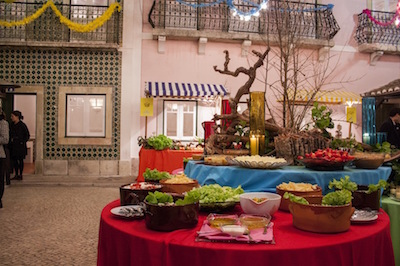
\includegraphics[height=3cm]{content/images-web/dinner-pateo-jantar-arraial}\ 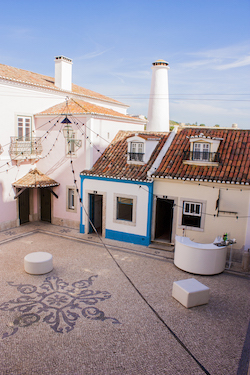
\includegraphics[height=3cm]{content/images-web/dinner-pateo-exterior}\ 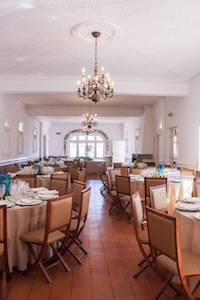
\includegraphics[height=3cm]{content/images-web/dinner-pateo-sala}
\par\end{center}

Páteo Alfacinha was created in 1981, featuring several spaces typical
from the beginning of XX century Lisbon: a chapel, a barber shop,
a tavern, a bakery, a pub, an antiquary, and houses for the “alfacinhas”
(inhabitants of Lisbon). Nowadays, Páteo Alfacinha remains a multifaceted
place, with restaurants and facilities for events such as EMNLP's
conference dinner.


\subsection*{Welcome Reception}

Friday, September 18th at 18:30 at Culturgest


\subsection*{Conference Dinner}

Sunday, September 20th at 19:00 at Pateo Alfacinha

First buses depart from Culturgest at 18:15. 

Last returning bus depart from Páteo Alfacinha at 24:00.


\subsection*{Farewell Drink}

Monday, September 21th at 18:30 at Culturgest



\chapter{\label{chap:Tutorials}Tutorials: Thursday -- Friday, September,
17--18}

\begin{longtable}{r>{\raggedright}p{0.83\columnwidth}}
 & \textbf{\large{}September 17\smallskip{}
}\tabularnewline
09:00 -- 12:30 & \textbf{Morning Tutorials}\tabularnewline
 & \linktutorial{tutorials-001}{\TutLocA}

\linktutorial{tutorials-002}{\TutLocB}\tabularnewline
12:30 -- 14:00 & \textbf{Lunch break}\tabularnewline
14:00 -- 17:30 & \textbf{Afternoon Tutorials}\tabularnewline
 & \linktutorial{tutorials-003}{\TutLocC}

\linktutorial{tutorials-004}{\TutLocD}\textbf{\large{}\bigskip{}
}\tabularnewline
 & \textbf{\large{}September 18\smallskip{}
}\tabularnewline
09:00 -- 12:30 & \textbf{Morning Tutorials}\tabularnewline
 & \linktutorial{tutorials-005}{\TutLocE}

\linktutorial{tutorials-006}{\TutLocF}\tabularnewline
12:30 -- 14:00 & \textbf{Lunch break}\tabularnewline
14:00 -- 17:30 & \textbf{Afternoon Tutorials}\tabularnewline
 & \linktutorial{tutorials-007}{\TutLocG}

\linktutorial{tutorials-008}{\TutLocH}\tabularnewline
\end{longtable}

\clearpage{}

\begin{bio}

\textbf{David Jurgens} is a postdoctoral scholar at McGill University.
He received his PhD from the University of California, Los Angeles.
His research interests include lexical semantics, word sense disambiguation,
latent attribute inference, and the relationship between language
and location. He is currently co-chairing the 2015 and 2016 International
Workshops on Semantic Evaluation (SemEval). His research has been
featured in the MIT Technology Review, Forbes, Business Insider, and
Schneier on Security.

\textbf{Mohammad Taher Pilehvar} is a postdoctoral scholar at Sapienza
University of Rome. He received his PhD from the same university under
the supervision of Roberto Navigli. He does research in multiple areas
of Lexical Semantics such as semantic similarity and Word Sense Disambiguation
(WSD). His main focus is on unified graph-based semantic similarity
measures and large-scale frameworks for the evaluation of WSD systems.
He has co-organized a task on Cross Level Semantic Similarity in SemEval-2014
(Jurgens et al., 2014) and is the first author of a paper on semantic
similarity that was nominated for the best paper award at ACL 2013
(Pilehvar et al., 2013).

\index{Jurgens, David} \index{Pilehvar, Mohammad Taher} 

\end{bio}

\begin{tutorial}{tutorials-001}{September 17, 2015 -- 09:00--12:30}
{\TutLocA}

Semantic similarity forms a central component in many NLP systems,
from lexical semantics, to part of speech tagging, to social media
analysis. Recent years have seen a renewed interest in developing
new similarity techniques, buoyed in part by work on embeddings and
by SemEval tasks in Semantic Textual Similarity and Cross-Level Semantic
Similarity. The increased interest has led to hundreds of techniques
for measuring semantic similarity, which makes it difficult for practitioners
to identify which state-of-the-art techniques are applicable and easily
integrated into projects and for researchers to identify which aspects
of the problem require future research.

This tutorial synthesizes the current state of the art for measuring
semantic similarity for all types of conceptual or textual pairs and
presents a broad overview of current techniques, what resources they
use, and the particular inputs or domains to which the methods are
most applicable. We survey methods ranging from corpus-based approaches
operating on massive or domains-specific corpora to those leveraging
structural information from expert-based or collaboratively-constructed
lexical resources. Furthermore, we review work on multiple similarity
tasks from sense-based comparisons to word, sentence, and document-sized
comparisons and highlight general-purpose methods capable of comparing
multiple types of inputs. Where possible, we also identify techniques
that have been demonstrated to successfully operate in multilingual
or cross-lingual settings.

Our tutorial provides a clear overview of currently-available tools
and their strengths for practitioners who need out of the box solutions
and provides researchers with an understanding of the limitations
of current state of the art and what open problems remain in the field.
Given the breadth of available approaches, participants will also
receive a detailed bibliography of approaches (including those not
directly covered in the tutorial), annotated according to the approaches
abilities, and pointers to when open-source implementations of the
algorithms may be obtained.

\end{tutorial} 

\clearpage{}

\begin{bio}

\textbf{Yair Neuman} (Ben-Gurion Univ. of the Negev) is the co-director
of the Behavioral Insights Research Lab at the University of Toronto
and a senior fellow at the Brain Sciences Foundation. Among his fields
of interest are the interface of NLP and psychology and the development
of novel cognitive-psychological technologies.

\index{Neuman, Yair} 

\end{bio}

\begin{tutorial}{tutorials-002}{September 17, 2015 -- 09:00--12:30}
{\TutLocB}

``Personality'' is a psychological concept describing the individual's
characteristic patterns of thought, emotion, and behavior. In the
context of Big Data and granular analytics, it is highly important
to measure the individual's personality dimensions as these may be
used for various practical applications. However, personality has
been traditionally studied by questionnaires and other forms of low
tech methodologies. The availability of textual data and the development
of powerful NLP technologies, invite the challenge of automatically
measuring personality dimensions for various applications from granular
analytics of customers to the forensic identification of potential
offenders. While there are emerging attempts to address this challenge,
these attempts almost exclusively focus on one theoretical model of
personality and on classification tasks limited when tagged data are
not available.

The major aim of the tutorial is to provide NLP researchers with an
introduction to personality theories that may empower their scope
of research. In addition, two secondary aims are to survey some recent
directions in computational personality and to point to future directions
in which the field may be developed (e.g. Textual Entailment for Personality
Analytics).

\end{tutorial} 

\clearpage{}

\begin{bio}

\textbf{Laura Chiticariu} is a Research Staff Member at IBM Research
– Almaden. She received her Ph.D from U.C. Santa Cruz in 2008. Her
current research focuses on improving developmental support in information
extraction systems.

\textbf{Yunyao Li} is a Research Staff Member and Research Manager
at IBM Research – Almaden. She received her Ph.D from the University
of Michigan, Ann Arbor in 2007. She is particularly interested in
designing, developing and analyzing large scale systems that are usable
by a wide spectrum of users. Towards this direction, her current research
focuses on enterprise-scale natural language processing.

\textbf{Frederick Reiss }is a Research Staff Member at IBM Research
– Almaden. He received his Ph.D. from U.C. Berkeley in 2006. His research
focuses on improving the scalability of text analytics in enterprise
applications.

\index{Chiticariu, Laura} \index{Li, Yunyao} \index{Reiss, Frederick} 

\end{bio}

\begin{tutorial}{tutorials-003}{September 17, 2015 -- 14:00--17:30}
{\TutLocC}

The rise of Big Data analytics over unstructured text has led to renewed
interest in information extraction (IE). These applications need effective
IE as a first step towards solving end-to-end real world problems
(e.g. biology, medicine, finance, media and entertainment, etc). Much
recent NLP research has focused on addressing specific IE problems
using a pipeline of multiple machine learning techniques. This approach
requires an analyst with the expertise to answer questions such as:
“What ML techniques should I combine to solve this problem?”; “What
features will be useful for the composite pipeline?”; and “Why is
my model giving the wrong answer on this document?”. The need for
this expertise creates problems in real world applications. It is
very difficult in practice to find an analyst who both understands
the real world problem and has deep knowledge of applied machine learning.
As a result, the real impact by current IE research does not match
up to the abundant opportunities available.

In this tutorial, we introduce the concept of transparent machine
learning. A transparent ML technique is one that:
\begin{itemize}
\item produces models that a typical real world use can read and understand;
\item uses algorithms that a typical real world user can understand; and
\item allows a real world user to adapt models to new domains.
\end{itemize}
The tutorial is aimed at IE researchers in both the academic and industry
communities who are interested in developing and applying transparent
ML.

\end{tutorial} 

\clearpage{}

\begin{bio}

\textbf{Marius Pasca} is a research scientist at Google. Current research
interests include the acquisition of factual information from unstructured
text within documents and queries, and its applications to Web search.

\index{Pasca, Marius} 

\end{bio}

\begin{tutorial}{tutorials-004}{September 17, 2015 -- 14:00--17:30}
{\TutLocD}

The identification of textual items, or documents, that best match
a user’s information need, as expressed in search queries, forms the
core functionality of information retrieval systems. Well-known challenges
are associated with understanding the intent behind user queries;
and, more importantly, with matching inherently-ambiguous queries
to documents that may employ lexically different phrases to convey
the same meaning. The conversion of semi-structured content from Wikipedia
and other resources into structured data produces knowledge potentially
more suitable to database-style queries and, ideally, to use in information
retrieval. In parallel, the availability of textual documents on the
Web enables an aggressive push towards the automatic acquisition of
various types of knowledge from text. Methods developed under the
umbrella of open-domain information extraction acquire open-domain
classes of instances and relations from Web text. The methods operate
over unstructured or semi-structured text available within collections
of Web documents, or over relatively more intriguing streams of anonymized
search queries. Some of the methods import the automatically-extracted
data into human-generated resources, or otherwise exploit existing
human-generated resources. In both cases, the goal is to expand the
coverage of the initial resources, thus providing information about
more of the topics that people in general, and Web search users in
particular, may be interested in.

\end{tutorial} 

\clearpage{}

\begin{bio}

\textbf{Preslav Nakov}, a Senior Scientist at the Qatar Computing
Research Institute, part of Qatar Foundation, holds a Ph.D. from the
University of California at Berkeley. His research interests include
computational linguistics and NLP, machine translation, lexical semantics,
Web as a corpus and biomedical text processing.

\textbf{Vivi Nastase} is a researcher at the Fondazione Bruno Kessler
in Trento, working mainly on lexical semantics, semantic relations,
knowledge acquisition and language evolution. She holds a Ph.D. from
the University of Ottawa, Canada.

\textbf{Diarmuid Ó Séaghdha}, Senior NLP Researcher at VocalIQ and
Visiting Industrial Fellow at the University of Cambridge, holds a
Ph.D. from the University of Cambridge. His research interests include
discourse and dialog, lexical and relational semantics, machine learning
for NLP, scientific text mining and social media analysis.

\textbf{Stan Szpakowicz}, an emeritus professor of Computer Science
at the University of Ottawa, holds a Ph.D. from the University of
Warsaw and a D.Sc. from the Polish Academy of Sciences. He has been
active in NLP since 1969. His recent interests include lexical resources,
semantic relations and emotion analysis.

\index{Nakov, Preslav} \index{Nastase Pilehvar, Vivi} \index{Ó Séaghdha, Diarmuid}
\index{Szpakowicz, Stan} 

\end{bio}

\begin{tutorial}{tutorials-005}{September 18, 2015 -- 09:00--12:30}
{\TutLocE}

Every non-trivial text describes interactions and relations between
people, institutions, activities, events and so on. What we know about
the world consists in large part of such relations, and that knowledge
contributes to the understanding of what texts refer to. Newly found
relations can in turn become part of this knowledge that is stored
for future use.

To grasp a text’s semantic content, an automatic system must be able
to recognize relations in texts and reason about them. This may be
done by applying and updating previously acquired knowledge. We focus
here in particular on semantic relations which describe the interactions
among nouns and compact noun phrases, and we present such relations
from both a theoretical and a practical perspective. The theoretical
exploration sketches the historical path which has brought us to the
contemporary view and interpretation of semantic relations. We discuss
a wide range of relation inventories proposed by linguists and by
language processing people. Such inventories vary by domain, granularity
and suitability for downstream applications.

On the practical side, we investigate the recognition and acquisition
of relations from texts. In a look at supervised learning methods,
we present available datasets, the variety of features which can describe
relation instances, and learning algorithms found appropriate for
the task.

Next, we present weakly supervised and unsupervised learning methods
of acquiring relations from large corpora with little or no previously
annotated data. We show how enduring the bootstrapping algorithm based
on seed examples or patterns has proved to be, and how it has been
adapted to tackle Web-scale text collections. We also show a few machine
learning techniques which can perform fast and reliable relation extraction
by taking advantage of data redundancy and variability.

\end{tutorial} 

\clearpage{}

\begin{bio}

Dr. \textbf{Atefeh Farzindar} is the CEO of NLP Technologies Inc.
and Adjunct Professor at University of Montreal. She has served as
Chair of the technology sector of the Language Industry Association
Canada (AILIA) (2009-2013), vice president of The Language Technologies
Research Centre (LTRC) of Canada (2012-2014) and a member of the Natural
Sciences and Engineering Research Council of Canada (NSERC) Computer
Science Liaison Committee (2014-2015). Recently, she authored a book
chapter in Social Network Integration in Document Summarization, Innovative
Document Summarization Techniques: Revolutionizing Knowledge Understanding,
IGI Global publisher January 2014.

Dr. \textbf{Diana Inkpen} is a Professor the School of Electrical
Engineering and Computer Science at the University of Ottawa. Her
research interests and expertise are in natural language processing,
in particular lexical semantics as applied to near synonyms and nuances
of meaning, word and text similarity, classification of texts by emotion
and mood, information retrieval from spontaneous speech, extraction
of semantic frames, and lexical choice in natural language generation.
She published more than 25 journal papers, 85 conference papers, and
6 book chapters. She is an associated editor of the Computational
Intelligence and Natural Language Engineering journals.

\index{Farzindar, Atefeh} \index{Inkpen, Diana} 

\end{bio}

\begin{tutorial}{tutorials-006}{September 18, 2015 -- 09:00--12:30}
{\TutLocF}

Analyzing social media texts is a complex problem that becomes difficult
to address using traditional Natural Language Processing (NLP) methods.
Our tutorial focuses on presenting new methods for NLP tasks and applications
that work on noisy and informal texts, such as the ones from social
media.

Automatic processing of large collections of social media texts is
important because they contain a lot of useful information, due to
the in-creasing popularity of all types of social media. Use of social
media and messaging apps grew 203 percent year-on-year in 2013, with
overall app use rising 115 percent over the same period, as reported
by Statista, citing data from Flurry Analytics. This growth means
that 1.61 billion people are now active in social media around the
world and this is expected to advance to 2 billion users in 2016,
led by India. The research shows that consumers are now spending daily
5.6 hours on digital media including social media and mo-bile internet
usage.

At the heart of this interest is the ability for users to create and
share content via a variety of platforms such as blogs, micro-blogs,
collaborative wikis, multimedia sharing sites, social net-working
sites. The unprecedented volume and variety of user-generated content,
as well as the user interaction network constitute new opportunities
for understanding social behavior and building socially intelligent
systems. Therefore it is important to investigate methods for knowledge
extraction from social media data. Furthermore, we can use this information
to detect and retrieve more related content about events, such as
photos and video clips that have caption texts.

\end{tutorial} 

\clearpage{}

\begin{bio}

\textbf{Miriam R. L. Petruck} received her PhD in Linguistics from
the University of California, Berkeley. A key member of the team developing
FrameNet almost since the project’s founding, her research interests
include semantics, knowledge base development, grammar and lexis,
lexical semantics, Frame Semantics and Construction Grammar

\textbf{Valia Kordoni} received her PhD in Computational Linguistics
from the University of Essex, UK. She joined the Department of English
Studies, Humboldt University Berlin in 2012, where she is Research
Professor of Linguistics. Her main research interests are in deep
linguistic processing, semantic analysis, and multiword expressions.

\index{Petruck, Miriam R. L.} \index{Kordoni, Valia} 

\end{bio}

\begin{tutorial}{tutorials-007}{September 18, 2015 -- 14:00--17:30}
{\TutLocG}

This tutorial will give participants a solid understanding of the
linguistic features of multiword expressions (MWEs), focusing on the
semantics of such expressions and their importance for natural language
processing and language technology, with particular attention to the
way that FrameNet (framenet.icsi.berkeley.edu) handles this wide spread
phenomenon. Our target audience includes researchers and practitioners
of language technology, not necessarily experts in MWEs or knowledgeable
about FrameNet, who are interested in NLP tasks that involve or could
benefit from considering MWEs as a pervasive phenomenon in human language
and communication.

NLP research has been interested in automatic processing of multiword
expressions, with reports on and tasks relating to such efforts presented
at workshops and conferences for at least ten years (e.g. ACL 2003,
LREC 2008, COLING 2010, EACL 2014). Overcoming the challenge of automatically
processing MWEs remains elusive in part because of the difficulty
in recognizing, acquiring, and interpreting such forms.

Indeed the phenomenon manifests in a range of linguistic forms (as
Sag et al. (2001), among many others, have documented), including:
noun + noun compounds (e.g. fish knife, health hazard etc.); adjective
+ noun compounds (e.g. political agenda, national interest, etc.);
particle verbs (shut up, take out, etc.); prepositional verbs (e.g.
look into, talk into, etc.); VP idioms, such as kick the bucket, and
pull someone’s leg, along with less obviously idiomatic forms like
answer the door, mention someone’s name, etc.; expressions that have
their own mini-grammars, such as names with honorifics and terms of
address (e.g. Rabbi Lord Jonathan Sacks), kinship terms (e.g. second
cousin once removed), and time expressions (e.g. January 9, 2015);
support verb constructions (e.g. verbs: take a bath, make a promise,
etc; and prepositions: in doubt, under review, etc.). Linguists address
issues of polysemy, compositionality, idiomaticity, and continuity
for each type included here.

While native speakers use these forms with ease, the treatment and
interpretation of MWEs in computational systems requires considerable
effort due to the very issues that concern linguists

\end{tutorial} \clearpage{}

\begin{bio}

\textbf{Saif Mohammad} has research interests in computational linguistics
and natural language processing, especially lexical semantics and
affect analysis. He develops computational models for sentiment analysis,
emotion detection, semantic distance, and lexical-semantic relations
such as word-pair antonymy. His team has developed a sentiment analysis
system which ranked first in SemEval shared tasks on the sentiment
analysis of tweets and on aspect-based sentiment analysis. His word-emotion
association resource, the NRC Emotion Lexicon, is widely used for
text analysis and information visualization. His recent work on generating
music from emotions in text garnered widespread media attention, including
articles in Time, LiveScience, io9, The Physics arXiv Blog, PC World,
and Popular Science.

\textbf{Cecilia Ovesdotter Alm} is a computational linguist dedicated
to advancing the understanding of affective and subjective meaning
across linguistic modalities and multimodal data. Her work focuses
on linguistic annotation and resource development for affect-related
problems, as well as computational modeling involving text and speech,
image understanding, and linguistic or multimodal sensing in this
area. She has published Affect in Text and Speech (2009) as well as
articles in proceedings and journals, representing over a decade of
related research.

\index{Mohammad, Saif} \index{Ovesdotter Alm, Cecilia} 

\end{bio}

\begin{tutorial}{tutorials-008}{September 18, 2015 -- 14:00--17:30}
{\TutLocH}

Computational linguistics has witnessed a surge of interest in approaches
to emotion and affect analysis, tackling problems that extend beyond
sentiment analysis in depth and complexity. This area involves basic
emotions (such as joy, sadness, and fear) as well as any of the hundreds
of other emotions humans are capable of (such as optimism, frustration,
and guilt), expanding into affective conditions, experiences, and
activities. Leveraging linguistic data for computational affect and
emotion inference enables opportunities to address a range of affect-related
tasks, problems, and non-invasive applications that capture aspects
essential to the human condition and individuals’ cognitive processes.
These efforts enable and facilitate human-centered computing experiences,
as demonstrated by applications across clinical, socio-political,
artistic, educational, and commercial domains. Efforts to computationally
detect, characterize, and generate emotions or affect-related phenomena
respond equally to technological needs for personalized, micro-level
analytics and broad-coverage, macro-level inference, and they have
involved both small and massive amounts of data.

While this is an exciting area with numerous opportunities for members
of the ACL community, a major obstacle is its intersection with other
investigatory traditions, necessitating knowledge transfer. This tutorial
comprehensively integrates relevant concepts and frameworks from linguistics,
cognitive science, affective computing, and computational linguistics
in order to equip researchers and practitioners with the adequate
background and knowledge to work effectively on problems and tasks
either directly involving, or benefiting from having an understanding
of, affect and emotion analysis.

There is a substantial body of work in traditional sentiment analysis
focusing on positive and negative sentiment. This tutorial covers
approaches and features that migrate well to affect analysis. We also
discuss key differences from sentiment analysis, and their implications
for analyzing affect and emotion.

The tutorial begins with an introduction that highlights opportunities,
key terminology, and interesting tasks and challenges (1). The body
of the tutorial covers characteristics of emotive language use with
emphasis on relevance for computational analysis (2); linguistic data—from
conceptual analysis frameworks via useful existing resources to important
annotation topics (3); computational approaches for lexical semantic
emotion analysis (4); computational approaches for emotion and affect
analysis in text (5); visualization methods (6); and a survey of application
areas with affect-related problems (7). The tutorial concludes with
an outline of future directions and a discussion with participants
about the areas relevant to their respective tasks of interest (8).

Besides attending the tutorial, tutorial participants receive electronic
copies of tutorial slides, a complete reference list, as well as a
categorized annotated bibliography that concentrates on seminal works,
recent important publications, and other products and resources for
researchers and developers.

\end{tutorial} 


%\setdaydateyear{Thursday -- Friday}{September 17 -- 18}{2015}


\chapter{Workshops\label{chap:Workshops}}

\begin{longtable}{l>{\raggedright}p{0.9\columnwidth}}
\multicolumn{2}{l}{\textbf{September 17th -- 18th, Thursday -- Friday}\hfill{}page}\tabularnewline
\midrule
MA & \linkworkshoptitle{WMT15}{WMT: } \tabularnewline
 & \tabularnewline
\multicolumn{2}{l}{\textbf{September 17th -- Thursday }}\tabularnewline
\midrule
\WShopLocB & \linkworkshoptitle{WASSA15}{WASSA: }\tabularnewline
\WShopLocC & \linkworkshoptitle{DiscoMT15}{DiscoMT: }\tabularnewline
\WShopLocD & \linkworkshoptitle{Louhi15}{LOUHI: }\tabularnewline
 & \tabularnewline
\multicolumn{2}{l}{\textbf{September 18th -- Friday }}\tabularnewline
\midrule
\WShopLocE & \linkworkshoptitle{LSDSem}{LSDSem: }\tabularnewline
\WShopLocF & \linkworkshoptitle{CogACLL}{CogACLL: }\tabularnewline
\WShopLocG & \linkworkshoptitle{VL15}{VL: }\tabularnewline
\end{longtable}

\begin{wsschedule}{WMT15}{WMT}{Tenth Workshop on Statistical Machine Translation}{\WShopLocA} 
\item[] {\Large\bfseries Thursday, September 17, 2015}\\\vspace{1ex}

\vspace{0.75ex}
\item[09:00--09:05] {\bfseries Opening Remarks}

\vspace{0.75ex}
\item[09:05--09:50] {\bfseries Session 1: Shared Tasks}

\vspace{0.5ex}
\item[$\bullet$] \wspaperentry{WMT15-079}

\vspace{0.75ex}
\item[09:50--10:30] {\bfseries Session 2: Data Selection}

\vspace{0.5ex}
\item[09:50--10:10] \wspaperentry{WMT15-001}

\vspace{0.5ex}
\item[10:10--10:30] \wspaperentry{WMT15-006}

\vspace{0.75ex}
\item[10:30--11:00] {\bfseries Coffee Break}

\vspace{0.75ex}
\item[11:00--12:30] {\bfseries Session 3: Poster Session - Shared Task: Automatic Post-Editing}

\vspace{0.5ex}
\item[$\bullet$] \wspaperentry{WMT15-042}

\vspace{0.5ex}
\item[$\bullet$] \wspaperentry{WMT15-004}

\vspace{0.5ex}
\item[$\bullet$] \wspaperentry{WMT15-038}

\vspace{0.75ex}
\item[11:00--12:30] {\bfseries Session 3: Poster Session - Shared Task: Translation}

\vspace{0.5ex}
\item[$\bullet$] \wspaperentry{WMT15-055}

\vspace{0.5ex}
\item[$\bullet$] \wspaperentry{WMT15-031}

\vspace{0.5ex}
\item[$\bullet$] \wspaperentry{WMT15-054}

\vspace{0.5ex}
\item[$\bullet$] \wspaperentry{WMT15-057}

\vspace{0.5ex}
\item[$\bullet$] \wspaperentry{WMT15-014}

\vspace{0.5ex}
\item[$\bullet$] \wspaperentry{WMT15-039}

\vspace{0.5ex}
\item[$\bullet$] \wspaperentry{WMT15-024}

\vspace{0.5ex}
\item[$\bullet$] \wspaperentry{WMT15-010}

\vspace{0.5ex}
\item[$\bullet$] \wspaperentry{WMT15-056}

\vspace{0.5ex}
\item[$\bullet$] \wspaperentry{WMT15-072}

\vspace{0.5ex}
\item[$\bullet$] \wspaperentry{WMT15-044}

\vspace{0.5ex}
\item[$\bullet$] \wspaperentry{WMT15-067}

\vspace{0.5ex}
\item[$\bullet$] \wspaperentry{WMT15-048}

\vspace{0.5ex}
\item[$\bullet$] \wspaperentry{WMT15-019}

\vspace{0.5ex}
\item[$\bullet$] \wspaperentry{WMT15-022}

\vspace{0.5ex}
\item[$\bullet$] \wspaperentry{WMT15-029}

\vspace{0.5ex}
\item[$\bullet$] \wspaperentry{WMT15-053}

\vspace{0.5ex}
\item[$\bullet$] \wspaperentry{WMT15-052}

\vspace{0.5ex}
\item[$\bullet$] \wspaperentry{WMT15-064}

\vspace{0.5ex}
\item[$\bullet$] \wspaperentry{WMT15-060}

\vspace{0.5ex}
\item[$\bullet$] \wspaperentry{WMT15-058}

\vspace{0.75ex}
\item[12:30--14:00] {\bfseries Lunch}

\vspace{0.75ex}
\item[14:00--15:30] {\bfseries Session 4: Invited Talk}

\vspace{0.5ex}
\item[14:00--15:30] \textit{A Practical Guide to Real-Time Neural Translation (Jacob Devlin)}

\vspace{0.75ex}
\item[15:30--16:00] {\bfseries Coffee Break}

\vspace{0.75ex}
\item[16:00--17:00] {\bfseries Session 5: Syntax-Based Translation and Rescoring}

\vspace{0.5ex}
\item[16:00--16:20] \wspaperentry{WMT15-023}

\vspace{0.5ex}
\item[16:20--16:40] \wspaperentry{WMT15-049}

\vspace{0.5ex}
\item[16:40--17:00] \wspaperentry{WMT15-028}
\vspace{7em}
\item[] {\Large\bfseries Friday, September 18, 2015}\\\vspace{1ex}

\vspace{0.75ex}
\item[09:00--09:50] {\bfseries Session 6: Shared Tasks}

\vspace{0.5ex}
\item[09:00--09:20] \textit{Overview of the Quality Estimation Task}

\vspace{0.5ex}
\item[$\bullet$] \wspaperentry{WMT15-046}

\vspace{0.5ex}
\item[$\bullet$] \wspaperentry{WMT15-047}

\vspace{0.75ex}
\item[09:50--10:30] {\bfseries Session 7: Translation Modeling}

\vspace{0.5ex}
\item[09:50--10:10] \wspaperentry{WMT15-003}

\vspace{0.5ex}
\item[10:10--10:30] \wspaperentry{WMT15-043}

\vspace{0.75ex}
\item[10:30--11:00] {\bfseries Coffee Break}

\vspace{0.75ex}
\item[11:00--12:30] {\bfseries Session 8: Poster Session - Shared Task: Metrics}

\vspace{0.5ex}
\item[$\bullet$] \wspaperentry{WMT15-076}

\vspace{0.5ex}
\item[$\bullet$] \wspaperentry{WMT15-037}

\vspace{0.5ex}
\item[$\bullet$] \wspaperentry{WMT15-040}

\vspace{0.5ex}
\item[$\bullet$] \wspaperentry{WMT15-071}

\vspace{0.5ex}
\item[$\bullet$] \wspaperentry{WMT15-008}

\vspace{0.5ex}
\item[$\bullet$] \wspaperentry{WMT15-005}

\vspace{0.5ex}
\item[$\bullet$] \wspaperentry{WMT15-036}

\vspace{0.5ex}
\item[$\bullet$] \wspaperentry{WMT15-045}

\vspace{0.5ex}
\item[$\bullet$] \wspaperentry{WMT15-012}

\vspace{0.5ex}
\item[$\bullet$] \wspaperentry{WMT15-027}

\vspace{0.75ex}
\item[11:00--12:30] {\bfseries Session 8: Poster Session - Shared Task: Quality Estimation}

\vspace{0.5ex}
\item[$\bullet$] \wspaperentry{WMT15-033}

\vspace{0.5ex}
\item[$\bullet$] \wspaperentry{WMT15-018}

\vspace{0.5ex}
\item[$\bullet$] \wspaperentry{WMT15-009}

\vspace{0.5ex}
\item[$\bullet$] \wspaperentry{WMT15-016}

\vspace{0.5ex}
\item[$\bullet$] \wspaperentry{WMT15-051}

\vspace{0.5ex}
\item[$\bullet$] \wspaperentry{WMT15-050}

\vspace{0.5ex}
\item[$\bullet$] \wspaperentry{WMT15-059}

\vspace{0.5ex}
\item[$\bullet$] \wspaperentry{WMT15-078}

\vspace{0.5ex}
\item[$\bullet$] \wspaperentry{WMT15-021}

\vspace{0.75ex}
\item[11:00--12:30] {\bfseries Session 8: Poster Session - Shared Task: Tuning}

\vspace{0.5ex}
\item[$\bullet$] \wspaperentry{WMT15-002}

\vspace{0.5ex}
\item[$\bullet$] \wspaperentry{WMT15-020}

\vspace{0.5ex}
\item[$\bullet$] \wspaperentry{WMT15-075}

\vspace{0.75ex}
\item[12:30--14:00] {\bfseries Lunch}

\vspace{0.75ex}
\item[14:00--15:20] {\bfseries Session 9: Evaluation and System Combination}

\vspace{0.5ex}
\item[$\bullet$] \wspaperentry{WMT15-032}

\vspace{0.5ex}
\item[$\bullet$] \wspaperentry{WMT15-035}

\vspace{0.5ex}
\item[$\bullet$] \wspaperentry{WMT15-062}

\vspace{0.5ex}
\item[$\bullet$] \wspaperentry{WMT15-011}

\vspace{0.75ex}
\item[15:20--16:00] {\bfseries Coffee Break}

\vspace{0.75ex}
\item[16:00--17:00] {\bfseries Session 10: Closing Session and Open Discussion}

\end{wsschedule}\begin{wsschedule}{WASSA15}{WASSA}{6th Workshop on Computational Approaches to Subjectivity, Sentiment and Social Media Analysis}{\WShopLocB} 
\item[] {\Large\bfseries Thursday, September 17, 2015}\\\vspace{1ex}

\vspace{0.75ex}
\item[09:00--09:05] {\bfseries Opening Remarks}

\vspace{0.75ex}
\item[09:05--09:40] {\bfseries Invited talk}

\vspace{0.5ex}
\item[$\bullet$] \wspaperentry{WASSA15-049}

\vspace{0.75ex}
\item[09:40--10:30] {\bfseries Session 1: Multilingual Sentiment Analysis in Social Media}

\vspace{0.5ex}
\item[09:40--10:10] \wspaperentry{WASSA15-001}

\vspace{0.5ex}
\item[10:10--10:30] \wspaperentry{WASSA15-043}

\vspace{0.75ex}
\item[10:30--11:00] {\bfseries Coffee Break}

\vspace{0.75ex}
\item[11:00--12:30] {\bfseries Session 2: The Influence of Context for Sentiment Analysis in Social Media}

\vspace{0.5ex}
\item[11:00--11:30] \wspaperentry{WASSA15-046}

\vspace{0.5ex}
\item[11:30--12:00] \wspaperentry{WASSA15-007}

\vspace{0.5ex}
\item[12:00--12:30] \wspaperentry{WASSA15-023}

\vspace{0.75ex}
\item[12:30--14:00] {\bfseries Lunch Break}

\vspace{0.75ex}
\item[14:00--15:30] {\bfseries Session 3: Beyond Review Mining}

\vspace{0.5ex}
\item[14:00--14:30] \wspaperentry{WASSA15-010}

\vspace{0.5ex}
\item[14:30--15:00] \wspaperentry{WASSA15-013}

\vspace{0.5ex}
\item[15:00--15:30] \wspaperentry{WASSA15-015}

\vspace{0.75ex}
\item[15:30--16:00] {\bfseries Coffee Break}

\vspace{0.75ex}
\item[16:00--17:20] {\bfseries Session 4: Lexicon Generation and Visualisation for Sentiment Analysis}

\vspace{0.5ex}
\item[16:00--16:30] \wspaperentry{WASSA15-033}

\vspace{0.5ex}
\item[16:30--17:00] \wspaperentry{WASSA15-037}

\vspace{0.5ex}
\item[17:00--17:20] \wspaperentry{WASSA15-028}

\vspace{0.75ex}
\item[17:20--17:30] {\bfseries Break}

\vspace{0.75ex}
\item[17:30--19:20] {\bfseries Session 5: Posters}

\vspace{0.5ex}
\item[$\bullet$] \wspaperentry{WASSA15-020}

\vspace{0.5ex}
\item[$\bullet$] \wspaperentry{WASSA15-006}

\vspace{0.5ex}
\item[$\bullet$] \wspaperentry{WASSA15-005}

\vspace{0.5ex}
\item[$\bullet$] \wspaperentry{WASSA15-019}

\vspace{0.5ex}
\item[$\bullet$] \wspaperentry{WASSA15-003}

\vspace{0.5ex}
\item[$\bullet$] \wspaperentry{WASSA15-004}

\vspace{0.5ex}
\item[$\bullet$] \wspaperentry{WASSA15-002}

\vspace{0.5ex}
\item[$\bullet$] \wspaperentry{WASSA15-045}

\vspace{0.5ex}
\item[$\bullet$] \wspaperentry{WASSA15-029}

\vspace{0.5ex}
\item[$\bullet$] \wspaperentry{WASSA15-032}

\vspace{0.5ex}
\item[$\bullet$] \wspaperentry{WASSA15-012}

\vspace{0.5ex}
\item[$\bullet$] \wspaperentry{WASSA15-038}

\vspace{0.5ex}
\item[$\bullet$] \wspaperentry{WASSA15-016}

\vspace{0.75ex}
\item[19:20--19:30] {\bfseries Closing discussion - "Where do we go from here?"}

\end{wsschedule}

\begin{wsschedule}{DiscoMT15}{DiscoMT}{Second Workshop on Discourse in Machine Translation}{\WShopLocC} 
\item[] {\Large\bfseries Thursday, September 17, 2015}\\\vspace{1ex}

\vspace{0.75ex}
\item[09:00--10:30] {\bfseries Session 1}

\vspace{0.5ex}
\item[09:00--09:05] \textit{Introduction (Bonnie Webber)}

\vspace{0.5ex}
\item[09:05--09:35] \wspaperentry{DiscoMT15-026}

\vspace{0.5ex}
\item[09:35--09:50] \wspaperentry{DiscoMT15-010}

\vspace{0.5ex}
\item[09:50--10:15] \wspaperentry{DiscoMT15-006}

\vspace{0.75ex}
\item[10:15--10:30] {\bfseries Poster Boaster}

\vspace{0.75ex}
\item[10:30--11:00] {\bfseries Coffee Break}

\vspace{0.75ex}
\item[11:00--12:30] {\bfseries Session 2a: Regular Track Posters}

\vspace{0.5ex}
\item[$\bullet$] \wspaperentry{DiscoMT15-018}

\vspace{0.5ex}
\item[$\bullet$] \wspaperentry{DiscoMT15-016}

\vspace{0.5ex}
\item[$\bullet$] \wspaperentry{DiscoMT15-012}

\vspace{0.5ex}
\item[$\bullet$] \wspaperentry{DiscoMT15-001}

\vspace{0.75ex}
\item[11:00--12:30] {\bfseries Session 2b: Posters Related to Oral Presentations}

\vspace{0.5ex}
\item[$\bullet$] \textit{On Statistical Machine Translation and Translation Theory (Christian Hardmeier)}

\vspace{0.5ex}
\item[$\bullet$] \textit{Exploration of Inter- and Intralingual Variation of Discourse Phenomena (Ekaterina Lapshinova-Koltunski)}

\vspace{0.5ex}
\item[$\bullet$] \textit{Measuring ’Registerness’ in Human and Machine Translation: A Text Classification Approach (Ekaterina Lapshinova-Koltunski and Mihaela Vela)}

\vspace{0.5ex}
\item[$\bullet$] \textit{Translation Model Adaptation Using Genre-Revealing Text Features (Marlies van der Wees, Arianna Bisazza, Christof Monz)}

\vspace{0.5ex}
\item[$\bullet$] \textit{Crosslingual Annotation and Analysis of Implicit Discourse Connectives for Machine Translation (Frances Yung, Kevin Duh, Yuji Matsumoto)}

\vspace{0.75ex}
\item[11:00--12:30] {\bfseries Session 2c: Shared Task Posters}

\vspace{0.5ex}
\item[$\bullet$] \wspaperentry{DiscoMT15-015}

\vspace{0.5ex}
\item[$\bullet$] \wspaperentry{DiscoMT15-008}

\vspace{0.5ex}
\item[$\bullet$] \wspaperentry{DiscoMT15-007}

\vspace{0.5ex}
\item[$\bullet$] \wspaperentry{DiscoMT15-014}

\vspace{0.5ex}
\item[$\bullet$] \wspaperentry{DiscoMT15-013}

\vspace{0.5ex}
\item[$\bullet$] \wspaperentry{DiscoMT15-005}

\vspace{0.5ex}
\item[$\bullet$] \wspaperentry{DiscoMT15-019}

\vspace{0.5ex}
\item[$\bullet$] \wspaperentry{DiscoMT15-021}

\vspace{0.5ex}
\item[$\bullet$] \wspaperentry{DiscoMT15-017}

\vspace{0.75ex}
\item[12:30--14:00] {\bfseries Lunch Break}

\vspace{0.75ex}
\item[14:00--15:30] {\bfseries Session 3}

\vspace{0.5ex}
\item[14:00--14:25] \wspaperentry{DiscoMT15-002}

\vspace{0.5ex}
\item[14:25--14:50] \wspaperentry{DiscoMT15-020}

\vspace{0.5ex}
\item[14:50--15:15] \wspaperentry{DiscoMT15-023}

\vspace{0.5ex}
\item[15:15--15:30] \wspaperentry{DiscoMT15-011}

\vspace{0.75ex}
\item[15:30--16:00] {\bfseries Coffee Break}

\vspace{0.75ex}
\item[16:00--17:30] {\bfseries Session 4}

\vspace{0.5ex}
\item[16:00--16:25] \wspaperentry{DiscoMT15-004}

\vspace{0.5ex}
\item[16:25--16:40] \wspaperentry{DiscoMT15-022}

\vspace{0.5ex}
\item[16:40--17:30] \textit{Final Discussions and Conclusions (Workshop Organizers and Audience)}

\end{wsschedule}

\begin{wsschedule}{Louhi15}{LOUHI}{Sixth Workshop on Health Text Mining and Information Analysis}{\WShopLocD} 
\item[] {\Large\bfseries Thursday, September 17, 2015}\\\vspace{1ex}

\vspace{0.75ex}
\item[09:00--10:30] {\bfseries Session I - Corpus creation}

\vspace{0.5ex}
\item[$\bullet$] \wspaperentry{Louhi15-015}

\vspace{0.5ex}
\item[$\bullet$] \wspaperentry{Louhi15-031}

\vspace{0.5ex}
\item[$\bullet$] \wspaperentry{Louhi15-032}

\vspace{0.5ex}
\item[$\bullet$] \wspaperentry{Louhi15-028}

\vspace{0.75ex}
\item[11:00--12:30] {\bfseries Session II - Poster}

\vspace{0.5ex}
\item[$\bullet$] \wspaperentry{Louhi15-002}

\vspace{0.5ex}
\item[$\bullet$] \wspaperentry{Louhi15-013}

\vspace{0.5ex}
\item[$\bullet$] \wspaperentry{Louhi15-016}

\vspace{0.5ex}
\item[$\bullet$] \wspaperentry{Louhi15-018}

\vspace{0.5ex}
\item[$\bullet$] \wspaperentry{Louhi15-021}

\vspace{0.5ex}
\item[$\bullet$] \wspaperentry{Louhi15-022}

\vspace{0.5ex}
\item[$\bullet$] \wspaperentry{Louhi15-024}

\vspace{0.5ex}
\item[$\bullet$] \wspaperentry{Louhi15-025}

\vspace{0.5ex}
\item[$\bullet$] \wspaperentry{Louhi15-027}

\vspace{0.5ex}
\item[$\bullet$] \wspaperentry{Louhi15-029}

\vspace{0.5ex}
\item[$\bullet$] \wspaperentry{Louhi15-042}

\vspace{0.75ex}
\item[12:30--14:00] {\bfseries Lunch break}

\vspace{0.75ex}
\item[14:00--15:30] {\bfseries Session III - Invited talk}

\vspace{0.5ex}
\item[$\bullet$] \wspaperentry{Louhi15-045}

\vspace{0.75ex}
\item[16:00--17:30] {\bfseries Session IV - Corpus processing}

\vspace{0.5ex}
\item[$\bullet$] \wspaperentry{Louhi15-005}

\vspace{0.5ex}
\item[$\bullet$] \wspaperentry{Louhi15-037}

\vspace{0.5ex}
\item[$\bullet$] \wspaperentry{Louhi15-039}

\vspace{0.5ex}
\item[$\bullet$] \wspaperentry{Louhi15-044}

\end{wsschedule}

\begin{wsschedule}{LSDSem}{LSDSem}{First Workshop on Linking Models of Lexical, Sentential and Discourse-level Semantics}{\WShopLocE} 
\item[] {\Large\bfseries Friday, September 18, 2015}\\\vspace{1ex}

\vspace{0.75ex}
\item[09:00--10:30] {\bfseries Morning Session}

\vspace{0.5ex}
\item[09:00--09:05] \textit{Introduction (Michael Roth)}

\vspace{0.5ex}
\item[09:05--09:50] \textit{Invited Talk: From Distributed Semantics to Discourse, and Back (Jacob Eisenstein)}

\vspace{0.5ex}
\item[09:50--10:05] \wspaperentry{LSDSem-012}

\vspace{0.5ex}
\item[10:05--10:20] \wspaperentry{LSDSem-014}

\vspace{0.5ex}
\item[10:20--10:30] \wspaperentry{LSDSem-020}

\vspace{0.75ex}
\item[10:30--11:00] {\bfseries Coffee Break}

\vspace{0.75ex}
\item[11:00--12:30] {\bfseries Pre-Lunch Session}

\vspace{0.5ex}
\item[11:00--11:15] \wspaperentry{LSDSem-005}

\vspace{0.5ex}
\item[11:15--11:30] \wspaperentry{LSDSem-026}

\vspace{0.5ex}
\item[11:30--11:45] \wspaperentry{LSDSem-013}

\vspace{0.5ex}
\item[11:45--11:55] \wspaperentry{LSDSem-019}

\vspace{0.5ex}
\item[11:55--12:05] \wspaperentry{LSDSem-017}

\vspace{0.5ex}
\item[12:05--12:15] \wspaperentry{LSDSem-023}

\vspace{0.5ex}
\item[12:15--12:25] \wspaperentry{LSDSem-027}

\vspace{0.75ex}
\item[12:30--14:00] {\bfseries Lunch Break}

\vspace{0.75ex}
\item[14:00--15:30] {\bfseries Post-Lunch Session}

\vspace{0.5ex}
\item[14:00--14:05] \textit{TextLink: EU COST action on Structuring Discourse in a Multi-Lingual Europe (Bonnie Webber)}

\vspace{0.5ex}
\item[14:05--14:50] \textit{Invited Talk: What Men Say, What Women Hear: Using Semantics To Make Better Sense of Gender Differences in Social Media (Rada Mihalcea)}

\vspace{0.5ex}
\item[14:50--15:00] \wspaperentry{LSDSem-025}

\vspace{0.5ex}
\item[15:00--15:10] \wspaperentry{LSDSem-011}

\vspace{0.75ex}
\item[15:10--16:00] {\bfseries Poster Session (Including Coffee Break)}

\vspace{0.75ex}
\item[15:30--16:00] {\bfseries Coffee Break}

\vspace{0.75ex}
\item[16:00--17:30] {\bfseries Afternoon Session}

\vspace{0.5ex}
\item[16:00--16:45] \textit{Invited Talk:  The (Non)Utility of Semantics for Coreference Resolution (Michael Strube)}

\vspace{0.5ex}
\item[16:45--17:30] \textit{Panel Discussion (Various speakers)}

\end{wsschedule}\begin{wsschedule}{CogACLL}{CogACLL}{Sixth Workshop on Cognitive Aspects of Computational Language Learning}{\WShopLocF}
\item[] {\Large\bfseries Friday, September 18, 2015}\\\vspace{1ex}

\vspace{0.75ex}
\item[09:00--09:10] {\bfseries Opening and Introduction}

\vspace{0.75ex}
\item[09:10--10:30] {\bfseries Session 1: Language Processing}

\vspace{0.5ex}
\item[09:10--09:30] \wspaperentry{CogACLL-014}

\vspace{0.5ex}
\item[09:30--10:00] \wspaperentry{CogACLL-016}

\vspace{0.5ex}
\item[10:00--10:30] \wspaperentry{CogACLL-027}

\vspace{0.75ex}
\item[10:30--11:00] {\bfseries Coffee Break}

\vspace{0.75ex}
\item[11:00--11:50] {\bfseries Invited Talk by Afra Alishahi}

\vspace{0.75ex}
\item[11:50--12:10] {\bfseries Session 2: Language  Change}

\vspace{0.5ex}
\item[11:50--12:10] \wspaperentry{CogACLL-017}

\vspace{0.75ex}
\item[12:10--13:00] {\bfseries Session 3: Poster Session}

\vspace{0.5ex}
\item[12:10--13:00] \wspaperentry{CogACLL-012}

\vspace{0.5ex}
\item[12:10--12:30] \wspaperentry{CogACLL-013}

\vspace{0.5ex}
\item[12:10--13:00] \wspaperentry{CogACLL-022}

\vspace{0.5ex}
\item[12:10--13:00] \wspaperentry{CogACLL-023}

\vspace{0.5ex}
\item[12:10--13:00] \wspaperentry{CogACLL-024}

\vspace{0.5ex}
\item[12:10--13:00] \wspaperentry{CogACLL-026}

\vspace{0.75ex}
\item[13:00--14:10] {\bfseries Lunch}

\vspace{0.75ex}
\item[14:10--15:00] {\bfseries Invited Talk by Antal van den Bosch}

\vspace{0.75ex}
\item[15:00--15:30] {\bfseries Session 4: Language Processing II}

\vspace{0.5ex}
\item[15:00--15:30] \wspaperentry{CogACLL-025}

\vspace{0.75ex}
\item[15:30--16:00] {\bfseries Coffee Break}

\vspace{0.75ex}
\item[16:00--17:30] {\bfseries Session 5: Language Acquisition}

\vspace{0.5ex}
\item[16:00--16:30] \wspaperentry{CogACLL-018}

\vspace{0.5ex}
\item[16:30--17:00] \wspaperentry{CogACLL-021}

\vspace{0.5ex}
\item[17:00--17:30] \wspaperentry{CogACLL-011}

\vspace{0.75ex}
\item[17:30--17:35] {\bfseries Closing Session}

\end{wsschedule}\begin{wsschedule}{VL15}{VL}{Fourth Workshop on Vision and Language}{\WShopLocG} 
\item[] {\Large\bfseries Friday, September 18, 2015}\\\vspace{1ex}

\vspace{0.75ex}
\item[08:45--10:30] {\bfseries Session 1}

\vspace{0.5ex}
\item[08:45--09:00] \textit{Opening Remarks (Marie-Francine Moens)}

\vspace{0.5ex}
\item[09:00--10:00] \textit{Invited Talk 1: Grounding Distributional Semantics in the Visual World (Marco Baroni)}

\vspace{0.75ex}
\item[10:00--10:30] {\bfseries Poster Spotlights 1}

\vspace{0.5ex}
\item[10:00--10:05] \wspaperentry{VL15-010}

\vspace{0.5ex}
\item[10:05--10:10] \wspaperentry{VL15-013}

\vspace{0.5ex}
\item[10:10--10:15] \wspaperentry{VL15-006}

\vspace{0.5ex}
\item[10:15--10:20] \wspaperentry{VL15-015}

\vspace{0.5ex}
\item[10:20--10:25] \wspaperentry{VL15-023}

\vspace{0.5ex}
\item[10:25--10:30] \wspaperentry{VL15-024}

\vspace{0.75ex}
\item[10:30--11:00] {\bfseries Coffee Break}

\vspace{0.75ex}
\item[11:00--12:15] {\bfseries Session 2}

\vspace{0.5ex}
\item[11:00--11:25] \wspaperentry{VL15-011}

\vspace{0.5ex}
\item[11:25--11:50] \wspaperentry{VL15-018}

\vspace{0.75ex}
\item[11:50--12:15] {\bfseries Poster Spotlights 2}

\vspace{0.5ex}
\item[11:50--11:55] \wspaperentry{VL15-026}

\vspace{0.5ex}
\item[11:55--12:00] \wspaperentry{VL15-008}

\vspace{0.5ex}
\item[12:00--12:05] \wspaperentry{VL15-017}

\vspace{0.5ex}
\item[12:05--12:10] \textit{Combining Geometric, Textual and Visual Features for Generating Prepositions in Image Descriptions (to appear in EMNLP 2015) (Arnau Ramisa, Josiah Wang, Ying Lu, Emmanuel Dellandrea, Francesc Moreno-Noguer and Robert Gaizauskas)}

\vspace{0.5ex}
\item[12:10--12:15] \textit{From the Virtual to the Real World: Referring to Visible Objects Under Uncertainty in Real-World Spatial Scenes (to appear in EMNLP 2015) (Dimitra Gkatzia and Verena Rieser)}

\vspace{0.75ex}
\item[12:15--14:00] {\bfseries Poster Session and Lunch}

\vspace{0.75ex}
\item[14:00--15:30] {\bfseries Session 3}

\vspace{0.5ex}
\item[14:00--15:00] \textit{Invited Talk 2: The ImageCLEF 2015 Task on Scalable Image Annotation, Localization and Sentence Generation (Krystian Mikolajczyk)}

\vspace{0.5ex}
\item[15:00--15:30] \wspaperentry{VL15-020}

\vspace{0.75ex}
\item[15:30--16:00] {\bfseries Coffee Break}

\vspace{0.75ex}
\item[16:00--18:00] {\bfseries Session 4}

\vspace{0.5ex}
\item[16:00--16:25] \wspaperentry{VL15-025}

\vspace{0.5ex}
\item[16:25--16:50] \wspaperentry{VL15-009}

\vspace{0.5ex}
\item[16:50--17:15] \wspaperentry{VL15-012}

\vspace{0.5ex}
\item[17:15--17:40] \wspaperentry{VL15-027}

\vspace{0.75ex}
\item[17:40--18:00] {\bfseries Closing Remarks and Discussion}

\end{wsschedule}

\chapter{Main Conference: Saturday, September 19}

\thispagestyle{emptyheader}


\section*{Overview}

\renewcommand{\arraystretch}{1.2}
\begin{SingleTrackSchedule}
  07:30 & -- & 18:00 &
  {\bfseries Registration} \hfill \emph{\RegistrationLoc}
  \\
  08:40 & -- & 10:00 &
  {\bfseries Session P1: Plenary Session} \hfill \emph{Main Auditorium}
  \\
 08:40 & -- & 09:00 & \textit{Opening Remarks and Introductory Speeches (General Chair, Program Co-Chairs and Local Co-Chairs)}\\
 09:00 & -- & 10:00 & \textit{Invited Talk: Deep Learning of Semantic Representations (Yoshua Bengio)}\\
  10:00 & -- & 10:30 &
  {\bfseries Coffee break} \hfill \emph{\CoffeeLoc}
  \\
  10:30 & -- & 12:10 &
  {\bfseries Session 1}\\

 & \multicolumn{3}{l}{%
 \begin{minipage}[t]{0.94\linewidth}
  \begin{tabular}{|>{\RaggedRight}p{0.235\linewidth}|>{\RaggedRight}p{0.235\linewidth}|>{\RaggedRight}p{0.235\linewidth}|>{\RaggedRight}p{0.235\linewidth}|}
  \hline
Semantics (Long + TACL Papers) & Machine Translation (Long + TACL Papers) & NLP for Web and Social Media, including Computational Social Science (Long Papers) & Long Paper Posters \rule{1\linewidth}{0.1pt} Short Paper Posters \\
\emph{\TrackALoc} & \emph{\TrackBLoc} & \emph{\TrackCLoc} & \emph{\TrackDLoc} \\
  \hline\end{tabular}
\end{minipage}
}\\
  12:10 & -- & 13:30 &
  {\bfseries Lunch} \hfill \emph{\LunchLoc}
  \\
  13:30 & -- & 15:10 &
  {\bfseries Session 2}\\

 & \multicolumn{3}{l}{%
 \begin{minipage}[t]{0.94\linewidth}
  \begin{tabular}{|>{\RaggedRight}p{0.235\linewidth}|>{\RaggedRight}p{0.235\linewidth}|>{\RaggedRight}p{0.235\linewidth}|>{\RaggedRight}p{0.235\linewidth}|}
  \hline
Statistical Models and Machine Learning Methods (Long + TACL Papers) & Tagging, Chunking and Parsing (Long +TACL Papers) & Summarization (Long Papers) & Long Paper Posters \rule{1\linewidth}{0.1pt} Short Paper Posters \\
\emph{\TrackALoc} & \emph{\TrackBLoc} & \emph{\TrackCLoc} & \emph{\TrackDLoc} \\
  \hline\end{tabular}
\end{minipage}
}\\
  15:10 & -- & 15:40 &
  {\bfseries Coffee break} \hfill \emph{\CoffeeLoc}
  \\
  15:40 & -- & 17:20 &
  {\bfseries Session 3}\\

 & \multicolumn{3}{l}{%
 \begin{minipage}[t]{0.94\linewidth}
  \begin{tabular}{|>{\RaggedRight}p{0.235\linewidth}|>{\RaggedRight}p{0.235\linewidth}|>{\RaggedRight}p{0.235\linewidth}|>{\RaggedRight}p{0.235\linewidth}|}
  \hline
Sentiment Analysis and Opinion Mining (Long Papers) & Semantics (Long +TACL Papers) & Information Retrieval and Question Answering (Long Papers) & Long + TACL Paper Posters \rule{1\linewidth}{0.1pt} Short Paper Posters \\
\emph{\TrackALoc} & \emph{\TrackBLoc} & \emph{\TrackCLoc} & \emph{\TrackDLoc} \\
  \hline\end{tabular}
\end{minipage}
}\\
\end{SingleTrackSchedule}


\clearpage{}


\section{Invited Speaker: Yoshua Bengio}

\index{Bengio, Yoshua}

\begin{center}
\textbf{\Large{}Deep Learning of Semantic Representations}{\Large{}\vspace{1em}
}
\par\end{center}{\Large \par}

\begin{center}
Saturday, September 19, 2015,  \vspace{1em}
\\
 \PlenaryLoc \\
 \vspace{1em}

\par\end{center}

\noindent \textbf{Abstract:} The core ingredient of deep learning
is the notion of distributed representation. This talk will start
by explaining its theoretical advantages, in comparison with non-parametric
methods based on counting frequencies of occurrence of observed tuples
of values (like with n-grams). The talk will then explain how having
multiple levels of representation, i.e., depth, can in principle give
another exponential advantage. Neural language models have been extremely
successful in recent years but extending their reach from language
modeling to machine translation is very appealing because it forces
the learned intermediate representations to capture meaning, and we
found that the resulting word embeddings are qualitatively different.
Recently, we introduced the notion of attention-based encoder-decoder
systems, with impressive results on machine translation several language
pairs and for mapping an image to a sentence, and these results will
conclude the talk.

\vspace{3em}


\vfill{}


\noindent \textbf{Biography:} Yoshua Bengio received a PhD in Computer
Science from McGill University, Canada in 1991. After two post-doctoral
years, one at M.I.T. with Michael Jordan and one at AT\&T Bell Laboratories
with Yann LeCun and Vladimir Vapnik, he became professor at the Department
of Computer Science and Operations Research at Université de Montréal.
He is the author of two books and more than 200 publications, the
most cited being in the areas of deep learning, recurrent neural networks,
probabilistic learning algorithms, natural language processing and
manifold learning. He is among the most cited Canadian computer scientists
and is or has been associate editor of the top journals in machine
learning and neural networks. Since '2000 he holds a Canada Research
Chair in Statistical Learning Algorithms, since '2006 an NSERC Industrial
Chair, since '2005 his is a Senior Fellow of the Canadian Institute
for Advanced Research and since 2014 he co-directs its program focused
on deep learning. He is on the board of the NIPS foundation and has
been program chair and general chair for NIPS. He has co-organized
the Learning Workshop for 14 years and co-created the new International
Conference on Learning Representations. His current interests are
centered around a quest for AI through machine learning, and include
fundamental questions on deep learning and representation learning,
the geometry of generalization in high-dimensional spaces, manifold
learning, biologically inspired learning algorithms, and challenging
applications of statistical machine learning.

\clearpage{}

\section[Session 1]{Session 1 Overview}
\begin{center}
\righthyphenmin2 \sloppy
\begin{tabular}{|p{0.33\columnwidth}|p{0.33\columnwidth}|p{0.33\columnwidth}|}
\hline
\bf Track A & \bf Track B & \bf Track C \\\hline
\it Semantics (Long + TACL Papers) & \it Machine Translation (Long + TACL Papers) & \it NLP for the Web and Social Media, including Computational Social Science (Long Papers) \\
\TrackALoc & \TrackBLoc & \TrackCLoc \\
\hline\hline
  \marginnote{\rotatebox{90}{10:30}}[2mm]
{}\papertableentry{papers-303} & {}\papertableentry{papers-444} & {}\papertableentry{papers-215}
  \\
  \hline
  \marginnote{\rotatebox{90}{10:55}}[2mm]
{}\papertableentry{papers-480} & {}\papertableentry{papers-501} & {}\papertableentry{papers-312}
  \\
  \hline
  \marginnote{\rotatebox{90}{11:20}}[2mm]
{}\papertableentry{papers-504} & {}\papertableentry{papers-630} & {}\papertableentry{papers-538}
  \\
  \hline
  \marginnote{\rotatebox{90}{11:45}}[2mm]
{[TACL] }\papertableentry{tacl-final-013} & {[TACL] }\papertableentry{tacl-final-003} & {}\papertableentry{papers-694}
  \\
\hline\end{tabular}\end{center}

\bigskip{}
\noindent \textbf{Track D:} \emph{Long Paper Posters} \hfill \emph{\sessionchair{Saif}{Mohammad}}\smallskip{}

\noindent {\PosterLoc \hfill \emph{10:30--12:10}}
\noindent \rule[0.5ex]{1\columnwidth}{1pt}
\begin{itemize}
\item []\textbf{Poster Cluster 1: Summarization (P1-4)}
\item \posterlistentry{papers-044}{}
\item \posterlistentry{papers-234}{}
\item \posterlistentry{papers-263}{}
\item \posterlistentry{papers-603}{}
\item []\textbf{Poster Cluster 2: Language and Vision (P5)}
\item \posterlistentry{papers-256}{}
\item []\textbf{Poster Cluster 3: Sentiment Analysis and Opinion Mining (P6-9)}
\item \posterlistentry{papers-089}{}
\item \posterlistentry{papers-152}{}
\item \posterlistentry{papers-617}{}
\item \posterlistentry{papers-646}{}
\end{itemize}

\bigskip{}
\noindent \textbf{Track E:} \emph{Short Paper Posters} \hfill \emph{\sessionchair{Kevin}{Duh}}\smallskip{}

\noindent {\PosterLoc \hfill \emph{10:30--12:10}}
\noindent \rule[0.5ex]{1\columnwidth}{1pt}
\begin{itemize}
\item []\textbf{Poster Cluster 1: Language and Vision (P1-3)}
\item \posterlistentry{papers-912}{}
\item \posterlistentry{papers-1268}{}
\item \posterlistentry{papers-1300}{}
\item []\textbf{Poster Cluster 2: Statistical Models and Machine Learning Methods (P4-16)}
\item \posterlistentry{papers-751}{}
\item \posterlistentry{papers-762}{}
\item \posterlistentry{papers-1048}{}
\item \posterlistentry{papers-1106}{}
\item \posterlistentry{papers-1125}{}
\item \posterlistentry{papers-1236}{}
\item \posterlistentry{papers-1246}{}
\item \posterlistentry{papers-1264}{}
\item \posterlistentry{papers-1342}{}
\item \posterlistentry{papers-1369}{}
\item \posterlistentry{papers-1381}{}
\item \posterlistentry{papers-1385}{}
\item \posterlistentry{papers-1457}{}
\end{itemize}

\clearpage

\newpage
\section*{Abstracts: Session 1}
\bigskip{}
\noindent{\bfseries\large Session 1A: Semantics (Long + TACL Papers)}\par
\noindent\TrackALoc\hfill\sessionchair{Yoav}{Artzi}\par
\bigskip{}
\paperabstract{papers-303}{10:30--10:55}{}
\paperabstract{papers-480}{10:55--11:20}{}
\paperabstract{papers-504}{11:20--11:45}{}
\paperabstract{tacl-final-013}{11:45--12:10}{[TACL] }
\clearpage
\noindent{\bfseries\large Session 1B: Machine Translation (Long + TACL Papers)}\par
\noindent\TrackBLoc\hfill\sessionchair{John}{DeNero}\par
\bigskip{}
\paperabstract{papers-444}{10:30--10:55}{}
\paperabstract{papers-501}{10:55--11:20}{}
\paperabstract{papers-630}{11:20--11:45}{}
\paperabstract{tacl-final-003}{11:45--12:10}{[TACL] }
\clearpage
\noindent{\bfseries\large Session 1C: NLP for the Web and Social Media, including Computational Social Science (Long Papers)}\par
\noindent\TrackCLoc\hfill\sessionchair{Brendan}{O'Connor}\par
\bigskip{}
\paperabstract{papers-215}{10:30--10:55}{}
\paperabstract{papers-312}{10:55--11:20}{}
\paperabstract{papers-538}{11:20--11:45}{}
\paperabstract{papers-694}{11:45--12:10}{}
\clearpage


\noindent{\bfseries\large Session 1D: Long Paper Posters} \hfill \emph{\sessionchair{Saif}{Mohammad}}\par
\noindent{\PosterLoc \hfill \emph{10:30--12:10}}\par
\bigskip{}
\posterabstract{papers-044}{}
\posterabstract{papers-234}{}
\posterabstract{papers-263}{}
\posterabstract{papers-603}{}
\posterabstract{papers-256}{}
\posterabstract{papers-089}{}
\posterabstract{papers-152}{}
\posterabstract{papers-617}{}
\posterabstract{papers-646}{}
\clearpage
\noindent{\bfseries\large Session 1E: Short Paper Posters} \hfill \emph{\sessionchair{Kevin}{Duh}}\par
\noindent{\PosterLoc \hfill \emph{10:30--12:10}}\par
\bigskip{}
\posterabstract{papers-912}{}
\posterabstract{papers-1268}{}
\posterabstract{papers-1300}{}
\posterabstract{papers-751}{}
\posterabstract{papers-762}{}
\posterabstract{papers-1048}{}
\posterabstract{papers-1106}{}
\posterabstract{papers-1125}{}
\posterabstract{papers-1236}{}
\posterabstract{papers-1246}{}
\posterabstract{papers-1264}{}
\posterabstract{papers-1342}{}
\posterabstract{papers-1369}{}
\posterabstract{papers-1381}{}
\posterabstract{papers-1385}{}
\posterabstract{papers-1457}{}
\clearpage

\section[Session 2]{Session 2 Overview}
\begin{center}
\righthyphenmin2 \sloppy
\begin{tabular}{|p{0.33\columnwidth}|p{0.33\columnwidth}|p{0.33\columnwidth}|}
\hline
\bf Track A & \bf Track B & \bf Track C \\\hline
\it Statistical Models and Machine Learning Methods (Long + TACL Papers) & \it Tagging, Chunking and Parsing (Long +TACL Papers) & \it Summarization (Long Papers) \\
\TrackALoc & \TrackBLoc & \TrackCLoc \\
\hline\hline
  \marginnote{\rotatebox{90}{13:30}}[2mm]
{}\papertableentry{papers-458} & {}\papertableentry{papers-054} & {}\papertableentry{papers-178}
  \\
  \hline
  \marginnote{\rotatebox{90}{13:55}}[2mm]
{}\papertableentry{papers-473} & {}\papertableentry{papers-162} & {}\papertableentry{papers-236}
  \\
  \hline
  \marginnote{\rotatebox{90}{14:20}}[2mm]
{}\papertableentry{papers-632} & {}\papertableentry{papers-524} & {}\papertableentry{papers-345}
  \\
  \hline
  \marginnote{\rotatebox{90}{14:45}}[2mm]
{[TACL] }\papertableentry{tacl-final-010} & {[TACL] }\papertableentry{tacl-final-016} & {}\papertableentry{papers-616}
  \\
\hline\end{tabular}\end{center}

\bigskip{}
\noindent \textbf{Track D:} \emph{Long Paper Posters} \hfill \emph{\sessionchair{Nate}{Chambers}}\smallskip{}

\noindent {\PosterLoc \hfill \emph{13:30--15:10}}
\noindent \rule[0.5ex]{1\columnwidth}{1pt}
\begin{itemize}
\item []\textbf{Poster Cluster 1: Text Mining and NLP Applications (P1-9)}
\item \posterlistentry{papers-102}{}
\item \posterlistentry{papers-259}{}
\item \posterlistentry{papers-432}{}
\item \posterlistentry{papers-445}{}
\item \posterlistentry{papers-475}{}
\item \posterlistentry{papers-507}{}
\item \posterlistentry{papers-544}{}
\item \posterlistentry{papers-608}{}
\item \posterlistentry{papers-614}{}
\end{itemize}

\bigskip{}
\noindent \textbf{Track E:} \emph{Short Paper Posters} \hfill \emph{\sessionchair{Wei}{Lu}}\smallskip{}

\noindent {\PosterLoc \hfill \emph{13:30--15:10}}
\noindent \rule[0.5ex]{1\columnwidth}{1pt}
\begin{itemize}
\item []\textbf{Poster Cluster 1: Information Extraction (P1-11)}
\item \posterlistentry{papers-821}{}
\item \posterlistentry{papers-902}{}
\item \posterlistentry{papers-995}{}
\item \posterlistentry{papers-1089}{}
\item \posterlistentry{papers-1183}{}
\item \posterlistentry{papers-1190}{}
\item \posterlistentry{papers-1267}{}
\item \posterlistentry{papers-1353}{}
\item \posterlistentry{papers-1383}{}
\item \posterlistentry{papers-1440}{}
\item \posterlistentry{papers-1464}{}
\item []\textbf{Poster Cluster 2: Information Retrieval and Question Answering (P12-16)}
\item \posterlistentry{papers-887}{}
\item \posterlistentry{papers-933}{}
\item \posterlistentry{papers-1249}{}
\item \posterlistentry{papers-1261}{}
\item \posterlistentry{papers-1389}{}
\end{itemize}

\clearpage

\newpage
\section*{Abstracts: Session 2}
\bigskip{}
\noindent{\bfseries\large Session 2A: Statistical Models and Machine Learning Methods (Long + TACL Papers)}\par
\noindent\TrackALoc\hfill\sessionchair{Alex}{Klementiev}\par
\bigskip{}
\paperabstract{papers-458}{13:30--13:55}{}
\paperabstract{papers-473}{13:55--14:20}{}
\paperabstract{papers-632}{14:20--14:45}{}
\paperabstract{tacl-final-010}{14:45--15:10}{[TACL] }
\clearpage
\noindent{\bfseries\large Session 2B: Tagging, Chunking and Parsing (Long +TACL Papers)}\par
\noindent\TrackBLoc\hfill\sessionchair{Eugene}{Charniak}\par
\bigskip{}
\paperabstract{papers-054}{13:30--13:55}{}
\paperabstract{papers-162}{13:55--14:20}{}
\paperabstract{papers-524}{14:20--14:45}{}
\paperabstract{tacl-final-016}{14:45--15:10}{[TACL] }
\clearpage
\noindent{\bfseries\large Session 2C: Summarization (Long Papers)}\par
\noindent\TrackCLoc\hfill\sessionchair{Yvette}{Graham}\par
\bigskip{}
\paperabstract{papers-178}{13:30--13:55}{}
\paperabstract{papers-236}{13:55--14:20}{}
\paperabstract{papers-345}{14:20--14:45}{}
\paperabstract{papers-616}{14:45--15:10}{}
\clearpage


\noindent{\bfseries\large Session 2D: Long Paper Posters} \hfill \emph{\sessionchair{Nate}{Chambers}}\par
\noindent{\PosterLoc \hfill \emph{13:30--15:10}}\par
\bigskip{}
\posterabstract{papers-102}{}
\posterabstract{papers-259}{}
\posterabstract{papers-432}{}
\posterabstract{papers-445}{}
\posterabstract{papers-475}{}
\posterabstract{papers-507}{}
\posterabstract{papers-544}{}
\posterabstract{papers-608}{}
\posterabstract{papers-614}{}
\clearpage
\noindent{\bfseries\large Session 2E: Short Paper Posters} \hfill \emph{\sessionchair{Wei}{Lu}}\par
\noindent{\PosterLoc \hfill \emph{13:30--15:10}}\par
\bigskip{}
\posterabstract{papers-821}{}
\posterabstract{papers-902}{}
\posterabstract{papers-995}{}
\posterabstract{papers-1089}{}
\posterabstract{papers-1183}{}
\posterabstract{papers-1190}{}
\posterabstract{papers-1267}{}
\posterabstract{papers-1353}{}
\posterabstract{papers-1383}{}
\posterabstract{papers-1440}{}
\posterabstract{papers-1464}{}
\posterabstract{papers-887}{}
\posterabstract{papers-933}{}
\posterabstract{papers-1249}{}
\posterabstract{papers-1261}{}
\posterabstract{papers-1389}{}
\clearpage

\section[Session 3]{Session 3 Overview}
\begin{center}
\righthyphenmin2 \sloppy
\begin{tabular}{|p{0.33\columnwidth}|p{0.33\columnwidth}|p{0.33\columnwidth}|}
\hline
\bf Track A & \bf Track B & \bf Track C \\\hline
\it Sentiment Analysis and Opinion Mining (Long Papers) & \it Semantics (Long +TACL Papers) & \it Information Retrieval and Question Answering (Long Papers) \\
\TrackALoc & \TrackBLoc & \TrackCLoc \\
\hline\hline
  \marginnote{\rotatebox{90}{15:40}}[2mm]
{}\papertableentry{papers-073} & {}\papertableentry{papers-536} & {}\papertableentry{papers-064}
  \\
  \hline
  \marginnote{\rotatebox{90}{16:05}}[2mm]
{}\papertableentry{papers-269} & {}\papertableentry{papers-635} & {}\papertableentry{papers-150}
  \\
  \hline
  \marginnote{\rotatebox{90}{16:30}}[2mm]
{}\papertableentry{papers-602} & {[TACL] }\papertableentry{tacl-final-001} & {}\papertableentry{papers-350}
  \\
  \hline
  \marginnote{\rotatebox{90}{16:55}}[2mm]
{}\papertableentry{papers-697} & {[TACL] }\papertableentry{tacl-final-018} & {}\papertableentry{papers-582}
  \\
\hline\end{tabular}\end{center}

\bigskip{}
\noindent \textbf{Track D:} \emph{Long + TACL Paper Posters} \hfill \emph{\sessionchair{Einat}{Minkov}}\smallskip{}

\noindent {\PosterLoc \hfill \emph{15:40--17:20}}
\noindent \rule[0.5ex]{1\columnwidth}{1pt}
\begin{itemize}
\item []\textbf{Poster Cluster 1: Information Extraction (P1-9)}
\item \posterlistentry{papers-221}{}
\item \posterlistentry{papers-232}{}
\item \posterlistentry{papers-385}{}
\item \posterlistentry{papers-453}{}
\item \posterlistentry{papers-474}{}
\item \posterlistentry{papers-526}{}
\item \posterlistentry{papers-708}{}
\item \posterlistentry{tacl-final-006}{[TACL] }
\item \posterlistentry{tacl-final-008}{[TACL] }
\end{itemize}

\bigskip{}
\noindent \textbf{Track E:} \emph{Short Paper Posters} \hfill \emph{\sessionchair{Wei}{Xu}}\smallskip{}

\noindent {\PosterLoc \hfill \emph{15:40--17:20}}
\noindent \rule[0.5ex]{1\columnwidth}{1pt}
\begin{itemize}
\item []\textbf{Poster Cluster 1: Text Mining and NLP Applications (P1-13)}
\item \posterlistentry{papers-1393}{}
\item \posterlistentry{papers-785}{}
\item \posterlistentry{papers-850}{}
\item \posterlistentry{papers-774}{}
\item \posterlistentry{papers-1062}{}
\item \posterlistentry{papers-1016}{}
\item \posterlistentry{papers-1120}{}
\item \posterlistentry{papers-1245}{}
\item \posterlistentry{papers-1156}{}
\item \posterlistentry{papers-1192}{}
\item \posterlistentry{papers-1336}{}
\item \posterlistentry{papers-776}{}
\item \posterlistentry{papers-777}{}
\end{itemize}

\clearpage

\newpage
\section*{Abstracts: Session 3}
\bigskip{}
\noindent{\bfseries\large Session 3A: Sentiment Analysis and Opinion Mining (Long Papers)}\par
\noindent\TrackALoc\hfill\sessionchair{Janyce}{Wiebe}\par
\bigskip{}
\paperabstract{papers-073}{15:40--16:05}{}
\paperabstract{papers-269}{16:05--16:30}{}
\paperabstract{papers-602}{16:30--16:55}{}
\paperabstract{papers-697}{16:55--17:20}{}
\clearpage
\noindent{\bfseries\large Session 3B: Semantics (Long +TACL Papers)}\par
\noindent\TrackBLoc\hfill\sessionchair{Regina}{Barzilay}\par
\bigskip{}
\paperabstract{papers-536}{15:40--16:05}{}
\paperabstract{papers-635}{16:05--16:30}{}
\paperabstract{tacl-final-001}{16:30--16:55}{[TACL] }
\paperabstract{tacl-final-018}{16:55--17:20}{[TACL] }
\clearpage
\noindent{\bfseries\large Session 3C: Information Retrieval and Question Answering (Long Papers)}\par
\noindent\TrackCLoc\hfill\sessionchair{Scott}{Wen-tau Yih}\par
\bigskip{}
\paperabstract{papers-064}{15:40--16:05}{}
\paperabstract{papers-150}{16:05--16:30}{}
\paperabstract{papers-350}{16:30--16:55}{}
\paperabstract{papers-582}{16:55--17:20}{}
\clearpage


\noindent{\bfseries\large Session 3D: Long + TACL Paper Posters} \hfill \emph{\sessionchair{Einat}{Minkov}}\par
\noindent{\PosterLoc \hfill \emph{15:40--17:20}}\par
\bigskip{}
\posterabstract{papers-221}{}
\posterabstract{papers-232}{}
\posterabstract{papers-385}{}
\posterabstract{papers-453}{}
\posterabstract{papers-474}{}
\posterabstract{papers-526}{}
\posterabstract{papers-708}{}
\posterabstract{tacl-final-006}{[TACL] }
\posterabstract{tacl-final-008}{[TACL] }
\clearpage
\noindent{\bfseries\large Session 3E: Short Paper Posters} \hfill \emph{\sessionchair{Wei}{Xu}}\par
\noindent{\PosterLoc \hfill \emph{15:40--17:20}}\par
\bigskip{}
\posterabstract{papers-1393}{}
\posterabstract{papers-785}{}
\posterabstract{papers-850}{}
\posterabstract{papers-774}{}
\posterabstract{papers-1062}{}
\posterabstract{papers-1016}{}
\posterabstract{papers-1120}{}
\posterabstract{papers-1245}{}
\posterabstract{papers-1156}{}
\posterabstract{papers-1192}{}
\posterabstract{papers-1336}{}
\posterabstract{papers-776}{}
\posterabstract{papers-777}{}
\clearpage



\chapter{Main Conference: Sunday, September 20}


\section*{Overview}

\renewcommand{\arraystretch}{1.2}
\begin{SingleTrackSchedule}
  07:30 & -- & 18:00 &
  {\bfseries Registration} \hfill \emph{\RegistrationLoc}
  \\
  08:00 & -- & 09:00 &
  {\bfseries Morning Coffee} \hfill \emph{\MorningLoc}
  \\
  09:00 & -- & 10:00 &
  {\bfseries Session P2: Plenary Session} \hfill \emph{Main Auditorium}
  \\
 & & & \textit{Invited Talk: Measuring How Elected Officials and Constituents Communicate (Justin Grimmer)}\\
  10:00 & -- & 10:30 &
  {\bfseries Coffee break} \hfill \emph{\CoffeeLoc}
  \\
  10:30 & -- & 12:10 &
  {\bfseries Session 4}\\

 & \multicolumn{3}{l}{%
 \begin{minipage}[t]{0.94\linewidth}
  \begin{tabular}{|>{\RaggedRight}p{0.235\linewidth}|>{\RaggedRight}p{0.235\linewidth}|>{\RaggedRight}p{0.235\linewidth}|>{\RaggedRight}p{0.235\linewidth}|}
  \hline
Information Extraction (Long Papers) & Statistical Models and Machine Learning Methods (Long Papers) & Discourse (Long +TACL Papers) & Long Paper Posters \rule{1\linewidth}{0.1pt} Short Paper Posters \\
\emph{\TrackALoc} & \emph{\TrackBLoc} & \emph{\TrackCLoc} & \emph{\TrackDLoc} \\
  \hline\end{tabular}
\end{minipage}
}\\
  12:10 & -- & 12:50 &
  {\bfseries Lunch} \hfill \emph{\LunchLoc}
  \\
  12:50 & -- & 13:30 &
  {\bfseries Session P3: SIGDAT business meeting} \hfill \emph{Main Auditorium}
  \\
  13:30 & -- & 15:10 &
  {\bfseries Session 5}\\

 & \multicolumn{3}{l}{%
 \begin{minipage}[t]{0.94\linewidth}
  \begin{tabular}{|>{\RaggedRight}p{0.235\linewidth}|>{\RaggedRight}p{0.235\linewidth}|>{\RaggedRight}p{0.235\linewidth}|>{\RaggedRight}p{0.235\linewidth}|}
  \hline
Text Mining and NLP Applications (Long + TACL Papers) & Semantics (Long +TACL Papers) & Phonology and Word Segmentation (Long Papers) & Long Paper Posters \rule{1\linewidth}{0.1pt} Short Paper Posters \\
\emph{\TrackALoc} & \emph{\TrackBLoc} & \emph{\TrackCLoc} & \emph{\TrackDLoc} \\
  \hline\end{tabular}
\end{minipage}
}\\
  15:10 & -- & 15:40 &
  {\bfseries Coffee break} \hfill \emph{\CoffeeLoc}
  \\
  15:40 & -- & 17:20 &
  {\bfseries Session 6}\\

 & \multicolumn{3}{l}{%
 \begin{minipage}[t]{0.94\linewidth}
  \begin{tabular}{|>{\RaggedRight}p{0.235\linewidth}|>{\RaggedRight}p{0.235\linewidth}|>{\RaggedRight}p{0.235\linewidth}|>{\RaggedRight}p{0.235\linewidth}|}
  \hline
Machine Translation (Long Papers) & Sentiment Analysis and Opinion Mining / Tagging, Chunking and Parsing (Long Papers) & Language and Vision / Information Extraction (Long Papers) & Long Paper Posters \rule{1\linewidth}{0.1pt} Short Paper Posters \\
\emph{\TrackALoc} & \emph{\TrackBLoc} & \emph{\TrackCLoc} & \emph{\TrackDLoc} \\
  \hline\end{tabular}
\end{minipage}
}\\
  19:00 & -- & 23:00 &
  {\bfseries Conference Dinner} \hfill \emph{Pateo Alfacinha}
  \\
\end{SingleTrackSchedule}


\clearpage{}


\section{Invited Speaker: Justin Grimmer}

\index{Bengio, Yoshua}

\begin{center}
\textbf{\Large{}Measuring How Elected Officials and Constituents Communicate}{\Large{}\vspace{1em}
}
\par\end{center}{\Large \par}

\begin{center}
Sunday, September 20, 2015,  \vspace{1em}
\\
 \PlenaryLoc \\
 \vspace{1em}

\par\end{center}

\noindent \textbf{Abstract:} This talk will show how elected officials
use communication to cultivate support with constituents, how constituents
express their views to elected officials, and why biases in both kinds
of communication matter for political representation. To demonstrate
the bias and its effects, I propose to use novel collections of political
texts and new text as data methods. Using the new data and methods,
I will show how the incentives of communication contribute to perceptions
of an angry public and vitriolic politicians. Among elected officials,
the ideologically extreme members of Congress disproportionately participate
in policy debates, resulting in political debates that occur between
the most extreme members of each party. Among constituents, the most
ideologically extreme and angry voters disproportionately contact
their member of Congress, creating the impression of a polarized and
vitriolic public. The talk will explain how the findings help us to
understand how representation occurs in American politics, while also
explaining how computational tools can help address questions in the
social sciences.

\vspace{3em}


\vfill{}


\noindent \textbf{Biography:} Justin Grimmer is an associate professor
of political science at Stanford University. His research examines
how representation occurs in American politics using new statistical
methods. His first book Representational Style in Congress: What Legislators
Say and Why It Matters (Cambridge University Press, 2013) shows how
senators define the type of representation they provide constituents
and how this affects constituents' evaluations and was awarded the
2014 Richard Fenno Prize. His second book The Impression of Influence:
How Legislator Communication and Government Spending Cultivate a Personal
Vote (Princeton University Press, 2014 with Sean J. Westwood and Solomon
Messing) demonstrates how legislators ensure they receive credit for
government actions. His work has appeared in the American Political
Science Review, American Journal of Political Science, Journal of
Politics, Political Analysis, Proceedings of the National Academy
of Sciences, Regulation and Governance, and Poetics.

\clearpage{}

\section[Session 4]{Session 4 Overview}
\begin{center}
\righthyphenmin2 \sloppy
\begin{tabular}{|p{0.33\columnwidth}|p{0.33\columnwidth}|p{0.33\columnwidth}|}
\hline
\bf Track A & \bf Track B & \bf Track C \\\hline
\it Information Extraction (Long Papers) & \it Statistical Models and Machine Learning Methods (Long Papers) & \it Discourse (Long +TACL Papers) \\
\TrackALoc & \TrackBLoc & \TrackCLoc \\
\hline\hline
  \marginnote{\rotatebox{90}{10:30}}[2mm]
{}\papertableentry{papers-080} & {}\papertableentry{papers-119} & {}\papertableentry{papers-417}
  \\
  \hline
  \marginnote{\rotatebox{90}{10:55}}[2mm]
{}\papertableentry{papers-352} & {}\papertableentry{papers-456} & {}\papertableentry{papers-568}
  \\
  \hline
  \marginnote{\rotatebox{90}{11:20}}[2mm]
{}\papertableentry{papers-595} & {}\papertableentry{papers-547} & {[TACL] }\papertableentry{tacl-final-004}
  \\
  \hline
  \marginnote{\rotatebox{90}{11:45}}[2mm]
{}\papertableentry{papers-707} & {}\papertableentry{papers-676} & {[TACL] }\papertableentry{tacl-final-012}
  \\
\hline\end{tabular}\end{center}

\bigskip{}
\noindent \textbf{Track D:} \emph{Long Paper Posters} \hfill \emph{\sessionchair{Sam}{Bowman}}\smallskip{}

\noindent {\PosterLoc \hfill \emph{10:30--12:10}}
\noindent \rule[0.5ex]{1\columnwidth}{1pt}
\begin{itemize}
\item []\textbf{Poster Cluster 1: Semantics (P1-8)}
\item \posterlistentry{papers-318}{}
\item \posterlistentry{papers-455}{}
\item \posterlistentry{papers-520}{}
\item \posterlistentry{papers-559}{}
\item \posterlistentry{papers-597}{}
\item \posterlistentry{papers-606}{}
\item \posterlistentry{papers-653}{}
\item \posterlistentry{papers-654}{}
\end{itemize}

\bigskip{}
\noindent \textbf{Track E:} \emph{Short Paper Posters} \hfill \emph{\sessionchair{Maja}{Popovic}}\smallskip{}

\noindent {\PosterLoc \hfill \emph{10:30--12:10}}
\noindent \rule[0.5ex]{1\columnwidth}{1pt}
\begin{itemize}
\item []\textbf{Poster Cluster 1: Machine Translation and Multilinguality (P1-13)}
\item \posterlistentry{papers-804}{}
\item \posterlistentry{papers-950}{}
\item \posterlistentry{papers-1058}{}
\item \posterlistentry{papers-1061}{}
\item \posterlistentry{papers-1078}{}
\item \posterlistentry{papers-1127}{}
\item \posterlistentry{papers-1222}{}
\item \posterlistentry{papers-1235}{}
\item \posterlistentry{papers-1275}{}
\item \posterlistentry{papers-1359}{}
\item \posterlistentry{papers-1451}{}
\item \posterlistentry{papers-1455}{}
\item \posterlistentry{papers-1470}{}
\item []\textbf{Poster Cluster 2: Computational Psycholinguistics (P14-16)}
\item \posterlistentry{papers-1274}{}
\item \posterlistentry{papers-1314}{}
\item \posterlistentry{papers-1323}{}
\end{itemize}

\clearpage

\newpage
\section*{Abstracts: Session 4}
\bigskip{}
\noindent{\bfseries\large Session 4A: Information Extraction (Long Papers)}\par
\noindent\TrackALoc\hfill\sessionchair{Heng}{Ji}\par
\bigskip{}
\paperabstract{papers-080}{10:30--10:55}{}
\paperabstract{papers-352}{10:55--11:20}{}
\paperabstract{papers-595}{11:20--11:45}{}
\paperabstract{papers-707}{11:45--12:10}{}
\clearpage
\noindent{\bfseries\large Session 4B: Statistical Models and Machine Learning Methods (Long Papers)}\par
\noindent\TrackBLoc\hfill\sessionchair{Chris}{Dyer}\par
\bigskip{}
\paperabstract{papers-119}{10:30--10:55}{}
\paperabstract{papers-456}{10:55--11:20}{}
\paperabstract{papers-547}{11:20--11:45}{}
\paperabstract{papers-676}{11:45--12:10}{}
\clearpage
\noindent{\bfseries\large Session 4C: Discourse (Long +TACL Papers)}\par
\noindent\TrackCLoc\hfill\sessionchair{Pascal}{Denis}\par
\bigskip{}
\paperabstract{papers-417}{10:30--10:55}{}
\paperabstract{papers-568}{10:55--11:20}{}
\paperabstract{tacl-final-004}{11:20--11:45}{[TACL] }
\paperabstract{tacl-final-012}{11:45--12:10}{[TACL] }
\clearpage


\noindent{\bfseries\large Session 4D: Long Paper Posters} \hfill \emph{\sessionchair{Sam}{Bowman}}\par
\noindent{\PosterLoc \hfill \emph{10:30--12:10}}\par
\bigskip{}
\posterabstract{papers-318}{}
\posterabstract{papers-455}{}
\posterabstract{papers-520}{}
\posterabstract{papers-559}{}
\posterabstract{papers-597}{}
\posterabstract{papers-606}{}
\posterabstract{papers-653}{}
\posterabstract{papers-654}{}
\clearpage
\noindent{\bfseries\large Session 4E: Short Paper Posters} \hfill \emph{\sessionchair{Maja}{Popovic}}\par
\noindent{\PosterLoc \hfill \emph{10:30--12:10}}\par
\bigskip{}
\posterabstract{papers-804}{}
\posterabstract{papers-950}{}
\posterabstract{papers-1058}{}
\posterabstract{papers-1061}{}
\posterabstract{papers-1078}{}
\posterabstract{papers-1127}{}
\posterabstract{papers-1222}{}
\posterabstract{papers-1235}{}
\posterabstract{papers-1275}{}
\posterabstract{papers-1359}{}
\posterabstract{papers-1451}{}
\posterabstract{papers-1455}{}
\posterabstract{papers-1470}{}
\posterabstract{papers-1274}{}
\posterabstract{papers-1314}{}
\posterabstract{papers-1323}{}
\clearpage

\section[Session 5]{Session 5 Overview}
\begin{center}
\righthyphenmin2 \sloppy
\begin{tabular}{|p{0.33\columnwidth}|p{0.33\columnwidth}|p{0.33\columnwidth}|}
\hline
\bf Track A & \bf Track B & \bf Track C \\\hline
\it Text Mining and NLP Applications (Long + TACL Papers) & \it Semantics (Long +TACL Papers) & \it Phonology and Word Segmentation (Long Papers) \\
\TrackALoc & \TrackBLoc & \TrackCLoc \\
\hline\hline
  \marginnote{\rotatebox{90}{13:30}}[2mm]
{[TACL] }\papertableentry{tacl-final-014} & {}\papertableentry{papers-222} & {}\papertableentry{papers-164}
  \\
  \hline
  \marginnote{\rotatebox{90}{13:55}}[2mm]
{}\papertableentry{papers-658} & {}\papertableentry{papers-564} & {}\papertableentry{papers-336}
  \\
  \hline
  \marginnote{\rotatebox{90}{14:20}}[2mm]
{[TACL] }\papertableentry{tacl-final-002} & {}\papertableentry{papers-615} & {}\papertableentry{papers-470}
  \\
  \hline
  \marginnote{\rotatebox{90}{14:45}}[2mm]
{[TACL] }\papertableentry{tacl-final-007} & {[TACL] }\papertableentry{tacl-final-017} & {}\papertableentry{papers-681}
  \\
\hline\end{tabular}\end{center}

\bigskip{}
\noindent \textbf{Track D:} \emph{Long Paper Posters} \hfill \emph{\sessionchair{Boxing}{Chen}}\smallskip{}

\noindent {\PosterLoc \hfill \emph{13:30--15:10}}
\noindent \rule[0.5ex]{1\columnwidth}{1pt}
\begin{itemize}
\item []\textbf{Poster Cluster 1: Machine Translation and Multilinguality (P1-8)}
\item \posterlistentry{papers-328}{}
\item \posterlistentry{papers-354}{}
\item \posterlistentry{papers-381}{}
\item \posterlistentry{papers-383}{}
\item \posterlistentry{papers-405}{}
\item \posterlistentry{papers-477}{}
\item \posterlistentry{papers-663}{}
\item \posterlistentry{papers-685}{}
\end{itemize}

\bigskip{}
\noindent \textbf{Track E:} \emph{Short Paper Posters} \hfill \emph{\sessionchair{Stephen}{Clark}}\smallskip{}

\noindent {\PosterLoc \hfill \emph{13:30--15:10}}
\noindent \rule[0.5ex]{1\columnwidth}{1pt}
\begin{itemize}
\item []\textbf{Poster Cluster 1: Tagging, Syntax and Parsing (P1-12)}
\item \posterlistentry{papers-794}{}
\item \posterlistentry{papers-837}{}
\item \posterlistentry{papers-839}{}
\item \posterlistentry{papers-895}{}
\item \posterlistentry{papers-968}{}
\item \posterlistentry{papers-1001}{}
\item \posterlistentry{papers-1238}{}
\item \posterlistentry{papers-1241}{}
\item \posterlistentry{papers-1301}{}
\item \posterlistentry{papers-1316}{}
\item \posterlistentry{papers-1368}{}
\item \posterlistentry{papers-1433}{}
\end{itemize}

\clearpage

\newpage
\section*{Abstracts: Parallel Session 5}
\bigskip{}
\noindent{\bfseries\large Session 5A: Text Mining and NLP Applications (Long + TACL Papers)}\par
\noindent\TrackALoc\hfill\sessionchair{Marie-Francine}{Moens}\par
\bigskip{}
\paperabstract{tacl-final-014}{13:30--13:55}{[TACL] }
\paperabstract{papers-658}{13:55--14:20}{}
\paperabstract{tacl-final-002}{14:20--14:45}{[TACL] }
\paperabstract{tacl-final-007}{14:45--15:10}{[TACL] }
\clearpage
\noindent{\bfseries\large Session 5B: Semantics (Long +TACL Papers)}\par
\noindent\TrackBLoc\hfill\sessionchair{Benjamin}{Van Durme}\par
\bigskip{}
\paperabstract{papers-222}{13:30--13:55}{}
\paperabstract{papers-564}{13:55--14:20}{}
\paperabstract{papers-615}{14:20--14:45}{}
\paperabstract{tacl-final-017}{14:45--15:10}{[TACL] }
\clearpage
\noindent{\bfseries\large Session 5C: Phonology and Word Segmentation (Long Papers)}\par
\noindent\TrackCLoc\hfill\sessionchair{Yue}{Zhang}\par
\bigskip{}
\paperabstract{papers-164}{13:30--13:55}{}
\paperabstract{papers-336}{13:55--14:20}{}
\paperabstract{papers-470}{14:20--14:45}{}
\paperabstract{papers-681}{14:45--15:10}{}
\clearpage


\noindent{\bfseries\large Session 5D: Long Paper Posters} \hfill \emph{\sessionchair{Boxing}{Chen}}\par
\noindent{\PosterLoc \hfill \emph{13:30--15:10}}\par
\bigskip{}
\posterabstract{papers-328}{}
\posterabstract{papers-354}{}
\posterabstract{papers-381}{}
\posterabstract{papers-383}{}
\posterabstract{papers-405}{}
\posterabstract{papers-477}{}
\posterabstract{papers-663}{}
\posterabstract{papers-685}{}
\clearpage
\noindent{\bfseries\large Session 5E: Short Paper Posters} \hfill \emph{\sessionchair{Stephen}{Clark}}\par
\noindent{\PosterLoc \hfill \emph{13:30--15:10}}\par
\bigskip{}
\posterabstract{papers-794}{}
\posterabstract{papers-837}{}
\posterabstract{papers-839}{}
\posterabstract{papers-895}{}
\posterabstract{papers-968}{}
\posterabstract{papers-1001}{}
\posterabstract{papers-1238}{}
\posterabstract{papers-1241}{}
\posterabstract{papers-1301}{}
\posterabstract{papers-1316}{}
\posterabstract{papers-1368}{}
\posterabstract{papers-1433}{}
\clearpage

\section[Session 6]{Session 6 Overview}
\begin{center}
\righthyphenmin2 \sloppy
\begin{tabular}{|p{0.33\columnwidth}|p{0.33\columnwidth}|p{0.33\columnwidth}|}
\hline
\bf Track A & \bf Track B & \bf Track C \\\hline
\it Machine Translation (Long Papers) & \it Sentiment Analysis and Opinion Mining / Tagging, Chunking and Parsing (Long Papers) & \it Language and Vision / Information Extraction (Long Papers) \\
\TrackALoc & \TrackBLoc & \TrackCLoc \\
\hline\hline
  \marginnote{\rotatebox{90}{15:40}}[2mm]
{}\papertableentry{papers-216} & {}\papertableentry{papers-011} & {}\papertableentry{papers-349}
  \\
  \hline
  \marginnote{\rotatebox{90}{16:05}}[2mm]
{}\papertableentry{papers-250} & {}\papertableentry{papers-651} & {}\papertableentry{papers-494}
  \\
  \hline
  \marginnote{\rotatebox{90}{16:30}}[2mm]
{}\papertableentry{papers-438} & {}\papertableentry{papers-465} & {}\papertableentry{papers-138}
  \\
  \hline
  \marginnote{\rotatebox{90}{16:55}}[2mm]
{}\papertableentry{papers-672} & {}\papertableentry{papers-636} & {}\papertableentry{papers-674}
  \\
\hline\end{tabular}\end{center}

\bigskip{}
\noindent \textbf{Track D:} \emph{Long Paper Posters} \hfill \emph{\sessionchair{Noah}{Smith}}\smallskip{}

\noindent {\PosterLoc \hfill \emph{15:40--17:20}}
\noindent \rule[0.5ex]{1\columnwidth}{1pt}
\begin{itemize}
\item []\textbf{Poster Cluster 1: Statistical Models and Machine Learning Methods (P1-11)}
\item \posterlistentry{papers-223}{}
\item \posterlistentry{papers-261}{}
\item \posterlistentry{papers-072}{}
\item \posterlistentry{papers-414}{}
\item \posterlistentry{papers-508}{}
\item \posterlistentry{papers-509}{}
\item \posterlistentry{papers-570}{}
\item \posterlistentry{papers-626}{}
\item \posterlistentry{papers-684}{}
\item \posterlistentry{papers-715}{}
\item \posterlistentry{papers-717}{}
\end{itemize}

\bigskip{}
\noindent \textbf{Track E:} \emph{Short Paper Posters} \hfill \emph{\sessionchair{Ido}{Dagan}}\smallskip{}

\noindent {\PosterLoc \hfill \emph{15:40--17:20}}
\noindent \rule[0.5ex]{1\columnwidth}{1pt}
\begin{itemize}
\item []\textbf{Poster Cluster 1: Semantics (P1-13)}
\item \posterlistentry{papers-827}{}
\item \posterlistentry{papers-865}{}
\item \posterlistentry{papers-872}{}
\item \posterlistentry{papers-920}{}
\item \posterlistentry{papers-921}{}
\item \posterlistentry{papers-926}{}
\item \posterlistentry{papers-945}{}
\item \posterlistentry{papers-1152}{}
\item \posterlistentry{papers-1184}{}
\item \posterlistentry{papers-1191}{}
\item \posterlistentry{papers-1304}{}
\item \posterlistentry{papers-1333}{}
\item \posterlistentry{papers-1394}{}
\end{itemize}

\clearpage

\newpage
\section*{Abstracts: Session 6}
\bigskip{}
\noindent{\bfseries\large Session 6A: Machine Translation (Long Papers)}\par
\noindent\TrackALoc\hfill\sessionchair{Lucia}{Specia}\par
\bigskip{}
\paperabstract{papers-216}{15:40--16:05}{}
\paperabstract{papers-250}{16:05--16:30}{}
\paperabstract{papers-438}{16:30--16:55}{}
\paperabstract{papers-672}{16:55--17:20}{}
\clearpage
\noindent{\bfseries\large Session 6B: Sentiment Analysis and Opinion Mining / Tagging, Chunking and Parsing (Long Papers)}\par
\noindent\TrackBLoc\hfill\sessionchair{Bing}{Liu and Dan Bikel}\par
\bigskip{}
\paperabstract{papers-011}{15:40--16:05}{}
\paperabstract{papers-651}{16:05--16:30}{}
\paperabstract{papers-465}{16:30--16:55}{}
\paperabstract{papers-636}{16:55--17:20}{}
\clearpage
\noindent{\bfseries\large Session 6C: Language and Vision / Information Extraction (Long Papers)}\par
\noindent\TrackCLoc\hfill\sessionchair{Meg}{Mitchell and Partha Talukdar}\par
\bigskip{}
\paperabstract{papers-349}{15:40--16:05}{}
\paperabstract{papers-494}{16:05--16:30}{}
\paperabstract{papers-138}{16:30--16:55}{}
\paperabstract{papers-674}{16:55--17:20}{}
\clearpage


\noindent{\bfseries\large Session 6D: Long Paper Posters} \hfill \emph{\sessionchair{Noah}{Smith}}\par
\noindent{\PosterLoc \hfill \emph{15:40--17:20}}\par
\bigskip{}
\posterabstract{papers-223}{}
\posterabstract{papers-261}{}
\posterabstract{papers-414}{}
\posterabstract{papers-508}{}
\posterabstract{papers-509}{}
\posterabstract{papers-570}{}
\posterabstract{papers-626}{}
\posterabstract{papers-684}{}
\posterabstract{papers-715}{}
\posterabstract{papers-717}{}
\clearpage
\noindent{\bfseries\large Session 6E: Short Paper Posters} \hfill \emph{\sessionchair{Ido}{Dagan}}\par
\noindent{\PosterLoc \hfill \emph{15:40--17:20}}\par
\bigskip{}
\posterabstract{papers-827}{}
\posterabstract{papers-865}{}
\posterabstract{papers-872}{}
\posterabstract{papers-920}{}
\posterabstract{papers-921}{}
\posterabstract{papers-926}{}
\posterabstract{papers-945}{}
\posterabstract{papers-1152}{}
\posterabstract{papers-1184}{}
\posterabstract{papers-1191}{}
\posterabstract{papers-1304}{}
\posterabstract{papers-1333}{}
\posterabstract{papers-1394}{}
\clearpage



\chapter{Main Conference: Monday, September 21}


\section*{Overview}

\renewcommand{\arraystretch}{1.2}
\begin{SingleTrackSchedule}
  07:30 & -- & 18:00 &
  {\bfseries Registration} \hfill \emph{\RegistrationLoc}
  \\
  08:00 & -- & 09:00 &
  {\bfseries Morning Coffee} \hfill \emph{\MorningLoc}
  \\
  09:00 & -- & 10:00 &
  {\bfseries Session P4: Plenary Session} \hfill \emph{Main Auditorium}
  \\
 09:00 & -- & 09:05 & \textit{Best Paper Awards (Chris Callison-Burch and Jian Su)}\\
 09:05 & -- & 09:30 & \paperlistentry{papers-662}\\
 09:30 & -- & 09:55 & \paperlistentry{papers-072}\\
 09:55 & -- & 10:05 & \paperlistentry{papers-536}\\
  10:05 & -- & 10:30 &
  {\bfseries Coffee break} \hfill \emph{\CoffeeLoc}
  \\
  10:30 & -- & 12:10 &
  {\bfseries Session 7}\\

 & \multicolumn{3}{l}{%
 \begin{minipage}[t]{0.94\linewidth}
  \begin{tabular}{|>{\RaggedRight}p{0.235\linewidth}|>{\RaggedRight}p{0.235\linewidth}|>{\RaggedRight}p{0.235\linewidth}|>{\RaggedRight}p{0.235\linewidth}|}
  \hline
Semantics (Long +TACL Papers) & Information Extraction (Long Papers) & Computational Psycholinguistics / Machine Translation (Long Papers) & Long +TACL Paper Posters \rule{1\linewidth}{0.1pt} Short Paper Posters \\
\emph{\TrackALoc} & \emph{\TrackBLoc} & \emph{\TrackCLoc} & \emph{\TrackDLoc} \\
  \hline\end{tabular}
\end{minipage}
}\\
  12:10 & -- & 13:30 &
  {\bfseries Lunch} \hfill \emph{\LunchLoc}
  \\
  13:30 & -- & 15:15 &
  {\bfseries Session 8}\\

 & \multicolumn{3}{l}{%
 \begin{minipage}[t]{0.94\linewidth}
  \begin{tabular}{|>{\RaggedRight}p{0.235\linewidth}|>{\RaggedRight}p{0.235\linewidth}|>{\RaggedRight}p{0.235\linewidth}|>{\RaggedRight}p{0.235\linewidth}|}
  \hline
Fun and Quirky Topics (Short Papers) & Semantics (Short Papers) & Statistical Models and Machine Learning Methods / Machine Translation (Short Papers) & Long Paper Posters \rule{1\linewidth}{0.1pt} Short Paper Posters \\
\emph{\TrackALoc} & \emph{\TrackBLoc} & \emph{\TrackCLoc} & \emph{\TrackDLoc} \\
  \hline\end{tabular}
\end{minipage}
}\\
  15:15 & -- & 15:40 &
  {\bfseries Coffee break} \hfill \emph{\CoffeeLoc}
  \\
  15:40 & -- & 17:20 &
  {\bfseries Session 9}\\

 & \multicolumn{3}{l}{%
 \begin{minipage}[t]{0.94\linewidth}
  \begin{tabular}{|>{\RaggedRight}p{0.235\linewidth}|>{\RaggedRight}p{0.235\linewidth}|>{\RaggedRight}p{0.235\linewidth}|>{\RaggedRight}p{0.235\linewidth}|}
  \hline
Statistical Models and Machine Learning Methods (Long + TACL Papers) & Text Mining and NLP Applications (Long Papers) & Spoken Language Processing and Language Modeling (Long Papers) & Long Paper Posters \rule{1\linewidth}{0.1pt} Short Paper Posters \\
\emph{\TrackALoc} & \emph{\TrackBLoc} & \emph{\TrackCLoc} & \emph{\TrackDLoc} \\
  \hline\end{tabular}
\end{minipage}
}\\
  17:30 & -- & 17:50 &
  {\bfseries Session P5: Closing Remarks} \hfill \emph{Main Auditorium}
  \\
  18:30 & -- & 20:00 &
  {\bfseries Farewell Drink} \hfill \emph{Culturgest}
  \\
\end{SingleTrackSchedule}


\clearpage{}

\newpage
\section*{Abstracts: Session P4}
\bigskip{}
\noindent{\bfseries\large Session P4: Plenary Session}\par
\noindent\TrackALoc\hfill\par
\bigskip{}
\paperabstract{papers-662}{09:05--09:30}{}
\paperabstract{papers-072}{09:30--09:55}{}
\paperabstract{papers-536}{09:55--10:05}{}
\clearpage



\section[Session 7]{Session 7 Overview}
\begin{center}
\righthyphenmin2 \sloppy
\begin{tabular}{|p{0.33\columnwidth}|p{0.33\columnwidth}|p{0.33\columnwidth}|}
\hline
\bf Track A & \bf Track B & \bf Track C \\\hline
\it Semantics (Long +TACL Papers) & \it Information Extraction (Long Papers) & \it Computational Psycholinguistics / Machine Translation (Long Papers) \\
\TrackALoc & \TrackBLoc & \TrackCLoc \\
\hline\hline
  \marginnote{\rotatebox{90}{10:30}}[2mm]
{}\papertableentry{papers-262} & {}\papertableentry{papers-165} & {}\papertableentry{papers-488}
  \\
  \hline
  \marginnote{\rotatebox{90}{10:55}}[2mm]
{}\papertableentry{papers-491} & {}\papertableentry{papers-195} & {}\papertableentry{papers-539}
  \\
  \hline
  \marginnote{\rotatebox{90}{11:20}}[2mm]
{}\papertableentry{papers-667} & {}\papertableentry{papers-553} & {}\papertableentry{papers-121}
  \\
  \hline
  \marginnote{\rotatebox{90}{11:45}}[2mm]
{[TACL] }\papertableentry{tacl-final-009} & {}\papertableentry{papers-579} & {}\papertableentry{papers-565}
  \\
\hline\end{tabular}\end{center}

\bigskip{}
\noindent \textbf{Track D:} \emph{Long +TACL Paper Posters} \hfill \emph{\sessionchair{David}{McClosky}}\smallskip{}

\noindent {\PosterLoc \hfill \emph{10:30--12:10}}
\noindent \rule[0.5ex]{1\columnwidth}{1pt}
\begin{itemize}
\item []\textbf{Poster Cluster 1: Word Segmentation, Tagging and Parsing (P1-6)}
\item \posterlistentry{papers-316}{}
\item \posterlistentry{papers-247}{}
\item \posterlistentry{papers-406}{}
\item \posterlistentry{papers-442}{}
\item \posterlistentry{papers-472}{}
\item \posterlistentry{tacl-final-015}{[TACL] }
\end{itemize}

\bigskip{}
\noindent \textbf{Track E:} \emph{Short Paper Posters} \hfill \emph{\sessionchair{Jun-Ping}{Ng}}\smallskip{}

\noindent {\PosterLoc \hfill \emph{10:30--12:10}}
\noindent \rule[0.5ex]{1\columnwidth}{1pt}
\begin{itemize}
\item []\textbf{Poster Cluster 1: Spoken Language Processing (P1-3)}
\item \posterlistentry{papers-908}{}
\item \posterlistentry{papers-1032}{}
\item \posterlistentry{papers-1211}{}
\item []\textbf{Poster Cluster 2: Summarization (P4-18)}
\item \posterlistentry{papers-806}{}
\item \posterlistentry{papers-812}{}
\item \posterlistentry{papers-941}{}
\item \posterlistentry{papers-952}{}
\item \posterlistentry{papers-1051}{}
\item \posterlistentry{papers-1060}{}
\item \posterlistentry{papers-1066}{}
\item \posterlistentry{papers-1081}{}
\item \posterlistentry{papers-1104}{}
\item \posterlistentry{papers-1133}{}
\item \posterlistentry{papers-1134}{}
\item \posterlistentry{papers-1161}{}
\item \posterlistentry{papers-1189}{}
\item \posterlistentry{papers-1203}{}
\item \posterlistentry{papers-1251}{}
\end{itemize}

\clearpage

\newpage
\section*{Abstracts: Session 7}
\bigskip{}
\noindent{\bfseries\large Session 7A: Semantics (Long +TACL Papers)}\par
\noindent\TrackALoc\hfill\sessionchair{Luke}{Zettlemoyer}\par
\bigskip{}
\paperabstract{papers-262}{10:30--10:55}{}
\paperabstract{papers-491}{10:55--11:20}{}
\paperabstract{papers-667}{11:20--11:45}{}
\paperabstract{tacl-final-009}{11:45--12:10}{[TACL] }
\clearpage
\noindent{\bfseries\large Session 7B: Information Extraction (Long Papers)}\par
\noindent\TrackBLoc\hfill\sessionchair{Shiqi}{Zhao}\par
\bigskip{}
\paperabstract{papers-165}{10:30--10:55}{}
\paperabstract{papers-195}{10:55--11:20}{}
\paperabstract{papers-553}{11:20--11:45}{}
\paperabstract{papers-579}{11:45--12:10}{}
\clearpage
\noindent{\bfseries\large Session 7C: Computational Psycholinguistics / Machine Translation (Long Papers)}\par
\noindent\TrackCLoc\hfill\sessionchair{Nizar}{Habash}\par
\bigskip{}
\paperabstract{papers-488}{10:30--10:55}{}
\paperabstract{papers-539}{10:55--11:20}{}
\paperabstract{papers-121}{11:20--11:45}{}
\paperabstract{papers-565}{11:45--12:10}{}
\clearpage


\noindent{\bfseries\large Session 7D: Long +TACL Paper Posters} \hfill \emph{\sessionchair{David}{McClosky}}\par
\noindent{\PosterLoc \hfill \emph{10:30--12:10}}\par
\bigskip{}
\posterabstract{papers-316}{}
\posterabstract{papers-247}{}
\posterabstract{papers-406}{}
\posterabstract{papers-442}{}
\posterabstract{papers-472}{}
\posterabstract{tacl-final-015}{[TACL] }
\clearpage
\noindent{\bfseries\large Session 7E: Short Paper Posters} \hfill \emph{\sessionchair{Jun-Ping}{Ng}}\par
\noindent{\PosterLoc \hfill \emph{10:30--12:10}}\par
\bigskip{}
\posterabstract{papers-908}{}
\posterabstract{papers-1032}{}
\posterabstract{papers-1211}{}
\posterabstract{papers-806}{}
\posterabstract{papers-812}{}
\posterabstract{papers-941}{}
\posterabstract{papers-952}{}
\posterabstract{papers-1051}{}
\posterabstract{papers-1060}{}
\posterabstract{papers-1066}{}
\posterabstract{papers-1081}{}
\posterabstract{papers-1104}{}
\posterabstract{papers-1133}{}
\posterabstract{papers-1134}{}
\posterabstract{papers-1161}{}
\posterabstract{papers-1189}{}
\posterabstract{papers-1203}{}
\posterabstract{papers-1251}{}
\clearpage

\section[Session 8]{Session 8 Overview}
\begin{center}
\righthyphenmin2 \sloppy
\begin{tabular}{|p{0.33\columnwidth}|p{0.33\columnwidth}|p{0.33\columnwidth}|}
\hline
\bf Track A & \bf Track B & \bf Track C \\\hline
\it Fun and Quirky Topics (Short Papers) & \it Semantics (Short Papers) & \it Statistical Models and Machine Learning Methods / Machine Translation (Short Papers) \\
\TrackALoc & \TrackBLoc & \TrackCLoc \\
\hline\hline
  \marginnote{\rotatebox{90}{13:30}}[2mm]
{}\papertableentry{papers-838} & {}\papertableentry{papers-835} & {}\papertableentry{papers-1311}
  \\
  \hline
  \marginnote{\rotatebox{90}{13:45}}[2mm]
{}\papertableentry{papers-760} & {}\papertableentry{papers-789} & {}\papertableentry{papers-755}
  \\
  \hline
  \marginnote{\rotatebox{90}{14:00}}[2mm]
{}\papertableentry{papers-853} & {}\papertableentry{papers-858} & {}\papertableentry{papers-1233}
  \\
  \hline
  \marginnote{\rotatebox{90}{14:15}}[2mm]
{}\papertableentry{papers-1302} & {}\papertableentry{papers-1145} & {}\papertableentry{papers-1295}
  \\
  \hline
  \marginnote{\rotatebox{90}{14:30}}[2mm]
{}\papertableentry{papers-873} & {}\papertableentry{papers-1231} & {}\papertableentry{papers-744}
  \\
  \hline
  \marginnote{\rotatebox{90}{14:45}}[2mm]
{}\papertableentry{papers-1352} & {}\papertableentry{papers-1422} & {}\papertableentry{papers-960}
  \\
  \hline
  \marginnote{\rotatebox{90}{15:00}}[2mm]
{}\papertableentry{papers-1109} &  & {}\papertableentry{papers-1294}
  \\
\hline\end{tabular}\end{center}

\bigskip{}
\noindent \textbf{Track D:} \emph{Long Paper Posters} \hfill \emph{\sessionchair{Tim}{Baldwin}}\smallskip{}

\noindent {\PosterLoc \hfill \emph{13:30--15:15}}
\noindent \rule[0.5ex]{1\columnwidth}{1pt}
\begin{itemize}
\item []\textbf{Poster Cluster 1: NLP for Web and Social Media, including Computational Social Science (P1-6)}
\item \posterlistentry{papers-228}{}
\item \posterlistentry{papers-249}{}
\item \posterlistentry{papers-459}{}
\item \posterlistentry{papers-481}{}
\item \posterlistentry{papers-598}{}
\item \posterlistentry{papers-621}{}
\item []\textbf{Poster Cluster 2: Discourse (P7-9)}
\item \posterlistentry{papers-363}{}
\item \posterlistentry{papers-587}{}
\item \posterlistentry{papers-677}{}
\end{itemize}

\bigskip{}
\noindent \textbf{Track E:} \emph{Short Paper Posters} \hfill \emph{\sessionchair{Owen}{Rambow}}\smallskip{}

\noindent {\PosterLoc \hfill \emph{13:30--15:15}}
\noindent \rule[0.5ex]{1\columnwidth}{1pt}
\begin{itemize}
\item []\textbf{Poster Cluster 1: Discourse (P1-9)}
\item \posterlistentry{papers-276}{}
\item \posterlistentry{papers-748}{}
\item \posterlistentry{papers-799}{}
\item \posterlistentry{papers-880}{}
\item \posterlistentry{papers-1041}{}
\item \posterlistentry{papers-1044}{}
\item \posterlistentry{papers-1056}{}
\item \posterlistentry{papers-1091}{}
\item \posterlistentry{papers-1115}{}
\item []\textbf{Poster Cluster 2: Phonology, Morphology and Word Segmentation (P10-15)}
\item \posterlistentry{papers-815}{}
\item \posterlistentry{papers-816}{}
\item \posterlistentry{papers-894}{}
\item \posterlistentry{papers-988}{}
\item \posterlistentry{papers-1391}{}
\item \posterlistentry{papers-1460}{}
\end{itemize}

\clearpage

\newpage
\section*{Abstracts: Session 8}
\bigskip{}
\noindent{\bfseries\large Session 8A: Fun and Quirky Topics (Short Papers)}\par
\noindent\TrackALoc\hfill\sessionchair{Yanjun}{Ma}\par
\bigskip{}
\paperabstract{papers-838}{13:30--13:45}{}
\paperabstract{papers-760}{13:45--14:00}{}
\paperabstract{papers-853}{14:00--14:15}{}
\paperabstract{papers-1302}{14:15--14:30}{}
\paperabstract{papers-873}{14:30--14:45}{}
\paperabstract{papers-1352}{14:45--15:00}{}
\paperabstract{papers-1109}{15:00--15:15}{}
\clearpage
\noindent{\bfseries\large Session 8B: Semantics (Short Papers)}\par
\noindent\TrackBLoc\hfill\sessionchair{Marco}{Baroni}\par
\bigskip{}
\paperabstract{papers-835}{13:30--13:45}{}
\paperabstract{papers-789}{13:45--14:00}{}
\paperabstract{papers-858}{14:00--14:15}{}
\paperabstract{papers-1145}{14:15--14:30}{}
\paperabstract{papers-1231}{14:30--14:45}{}
\paperabstract{papers-1422}{15:00--15:15}{}
\clearpage
\noindent{\bfseries\large Session 8C: Statistical Models and Machine Learning Methods / Machine Translation (Short Papers)}\par
\noindent\TrackCLoc\hfill\sessionchair{Kevin}{Gimpel}\par
\bigskip{}
\paperabstract{papers-1311}{13:30--13:45}{}
\paperabstract{papers-755}{13:45--14:00}{}
\paperabstract{papers-1233}{14:00--14:15}{}
\paperabstract{papers-1295}{14:15--14:30}{}
\paperabstract{papers-744}{14:30--14:45}{}
\paperabstract{papers-960}{14:45--15:00}{}
\paperabstract{papers-1294}{15:00--15:15}{}
\clearpage


\noindent{\bfseries\large Session 8D: Long Paper Posters} \hfill \emph{\sessionchair{Tim}{Baldwin}}\par
\noindent{\PosterLoc \hfill \emph{13:30--15:15}}\par
\bigskip{}
\posterabstract{papers-228}{}
\posterabstract{papers-249}{}
\posterabstract{papers-459}{}
\posterabstract{papers-481}{}
\posterabstract{papers-598}{}
\posterabstract{papers-621}{}
\posterabstract{papers-363}{}
\posterabstract{papers-587}{}
\posterabstract{papers-677}{}
\clearpage
\noindent{\bfseries\large Session 8E: Short Paper Posters} \hfill \emph{\sessionchair{Owen}{Rambow}}\par
\noindent{\PosterLoc \hfill \emph{13:30--15:15}}\par
\bigskip{}
\posterabstract{papers-276}{}
\posterabstract{papers-748}{}
\posterabstract{papers-799}{}
\posterabstract{papers-880}{}
\posterabstract{papers-1041}{}
\posterabstract{papers-1044}{}
\posterabstract{papers-1056}{}
\posterabstract{papers-1091}{}
\posterabstract{papers-1115}{}
\posterabstract{papers-815}{}
\posterabstract{papers-816}{}
\posterabstract{papers-894}{}
\posterabstract{papers-988}{}
\posterabstract{papers-1391}{}
\posterabstract{papers-1460}{}
\clearpage

\section[Session 9]{Session 9 Overview}
\begin{center}
\righthyphenmin2 \sloppy
\begin{tabular}{|p{0.33\columnwidth}|p{0.33\columnwidth}|p{0.33\columnwidth}|}
\hline
\bf Track A & \bf Track B & \bf Track C \\\hline
\it Statistical Models and Machine Learning Methods (Long + TACL Papers) & \it Text Mining and NLP Applications (Long Papers) & \it Spoken Language Processing and Language Modeling (Long Papers) \\
\TrackALoc & \TrackBLoc & \TrackCLoc \\
\hline\hline
  \marginnote{\rotatebox{90}{15:40}}[2mm]
{}\papertableentry{papers-060} & {}\papertableentry{papers-147} & {}\papertableentry{papers-258}
  \\
  \hline
  \marginnote{\rotatebox{90}{16:05}}[2mm]
{}\papertableentry{papers-323} & {}\papertableentry{papers-454} & {}\papertableentry{papers-580}
  \\
  \hline
  \marginnote{\rotatebox{90}{16:30}}[2mm]
{}\papertableentry{papers-588} & {}\papertableentry{papers-660} & {}\papertableentry{papers-638}
  \\
  \hline
  \marginnote{\rotatebox{90}{16:55}}[2mm]
{[TACL] }\papertableentry{tacl-final-011} & {}\papertableentry{papers-315} & {}\papertableentry{papers-382}
  \\
\hline\end{tabular}\end{center}

\bigskip{}
\noindent \textbf{Track D:} \emph{Long Paper Posters} \hfill \emph{\sessionchair{Nathan}{Schneider}}\smallskip{}

\noindent {\PosterLoc \hfill \emph{15:40--17:20}}
\noindent \rule[0.5ex]{1\columnwidth}{1pt}
\begin{itemize}
\item []\textbf{Poster Cluster 1: Semantics (P1-8)}
\item \posterlistentry{papers-105}{}
\item \posterlistentry{papers-109}{}
\item \posterlistentry{papers-116}{}
\item \posterlistentry{papers-181}{}
\item \posterlistentry{papers-185}{}
\item \posterlistentry{papers-204}{}
\item \posterlistentry{papers-243}{}
\item \posterlistentry{papers-308}{}
\end{itemize}

\bigskip{}
\noindent \textbf{Track E:} \emph{Short Paper Posters} \hfill \emph{\sessionchair{Kang}{Liu}}\smallskip{}

\noindent {\PosterLoc \hfill \emph{15:40--17:20}}
\noindent \rule[0.5ex]{1\columnwidth}{1pt}
\begin{itemize}
\item []\textbf{Poster Cluster 1: Sentiment Analysis and Opinion Mining (P1-9)}
\item \posterlistentry{papers-772}{}
\item \posterlistentry{papers-796}{}
\item \posterlistentry{papers-832}{}
\item \posterlistentry{papers-1040}{}
\item \posterlistentry{papers-1065}{}
\item \posterlistentry{papers-1090}{}
\item \posterlistentry{papers-1313}{}
\item \posterlistentry{papers-1331}{}
\item \posterlistentry{papers-1387}{}
\item []\textbf{Poster Cluster 2: NLP for the Web and Social Media, including Computational Social Science (P10-17)}
\item \posterlistentry{papers-943}{}
\item \posterlistentry{papers-983}{}
\item \posterlistentry{papers-994}{}
\item \posterlistentry{papers-1139}{}
\item \posterlistentry{papers-1149}{}
\item \posterlistentry{papers-1188}{}
\item \posterlistentry{papers-1361}{}
\end{itemize}

\clearpage

\newpage
\section*{Abstracts: Parallel Session 9}
\bigskip{}
\noindent{\bfseries\large Session 9A: Statistical Models and Machine Learning Methods (Long + TACL Papers)}\par
\noindent\TrackALoc\hfill\sessionchair{Jason}{Eisner}\par
\bigskip{}
\paperabstract{papers-060}{15:40--16:05}{}
\paperabstract{papers-323}{16:05--16:30}{}
\paperabstract{papers-588}{16:30--16:55}{}
\paperabstract{tacl-final-011}{16:55--17:20}{[TACL] }
\clearpage
\noindent{\bfseries\large Session 9B: Text Mining and NLP Applications (Long Papers)}\par
\noindent\TrackBLoc\hfill\sessionchair{Shuming}{Shi}\par
\bigskip{}
\paperabstract{papers-147}{15:40--16:05}{}
\paperabstract{papers-454}{16:05--16:30}{}
\paperabstract{papers-660}{16:30--16:55}{}
\paperabstract{papers-315}{16:55--17:20}{}
\clearpage
\noindent{\bfseries\large Session 9C: Spoken Language Processing and Language Modeling (Long Papers)}\par
\noindent\TrackCLoc\hfill\sessionchair{Isabel}{Trancoso}\par
\bigskip{}
\paperabstract{papers-258}{15:40--16:05}{}
\paperabstract{papers-580}{16:05--16:30}{}
\paperabstract{papers-638}{16:30--16:55}{}
\paperabstract{papers-382}{16:55--17:20}{}
\clearpage


\noindent{\bfseries\large Session 9D: Long Paper Posters} \hfill \emph{\sessionchair{Nathan}{Schneider}}\par
\noindent{\PosterLoc \hfill \emph{15:40--17:20}}\par
\bigskip{}
\posterabstract{papers-105}{}
\posterabstract{papers-109}{}
\posterabstract{papers-116}{}
\posterabstract{papers-181}{}
\posterabstract{papers-185}{}
\posterabstract{papers-204}{}
\posterabstract{papers-243}{}
\posterabstract{papers-308}{}
\clearpage
\noindent{\bfseries\large Session 9E: Short Paper Posters} \hfill \emph{\sessionchair{Kang}{Liu}}\par
\noindent{\PosterLoc \hfill \emph{15:40--17:20}}\par
\bigskip{}
\posterabstract{papers-772}{}
\posterabstract{papers-796}{}
\posterabstract{papers-832}{}
\posterabstract{papers-1040}{}
\posterabstract{papers-1065}{}
\posterabstract{papers-1090}{}
\posterabstract{papers-1313}{}
\posterabstract{papers-1331}{}
\posterabstract{papers-1387}{}
\posterabstract{papers-943}{}
\posterabstract{papers-983}{}
\posterabstract{papers-994}{}
\posterabstract{papers-1139}{}
\posterabstract{papers-1149}{}
\posterabstract{papers-1188}{}
\posterabstract{papers-1361}{}
\clearpage



\cleardoublepage{}

\phantomsection
\addcontentsline{toc}{chapter}{Author index}\printindex{}

\pagestyle{empty}

\clearpage{}

\phantomsection
\addcontentsline{toc}{chapter}{Sponsor Ads}\clearpage{}

\phantomsection
\addcontentsline{toc}{chapter}{Sponsor Ads}

\begin{center}
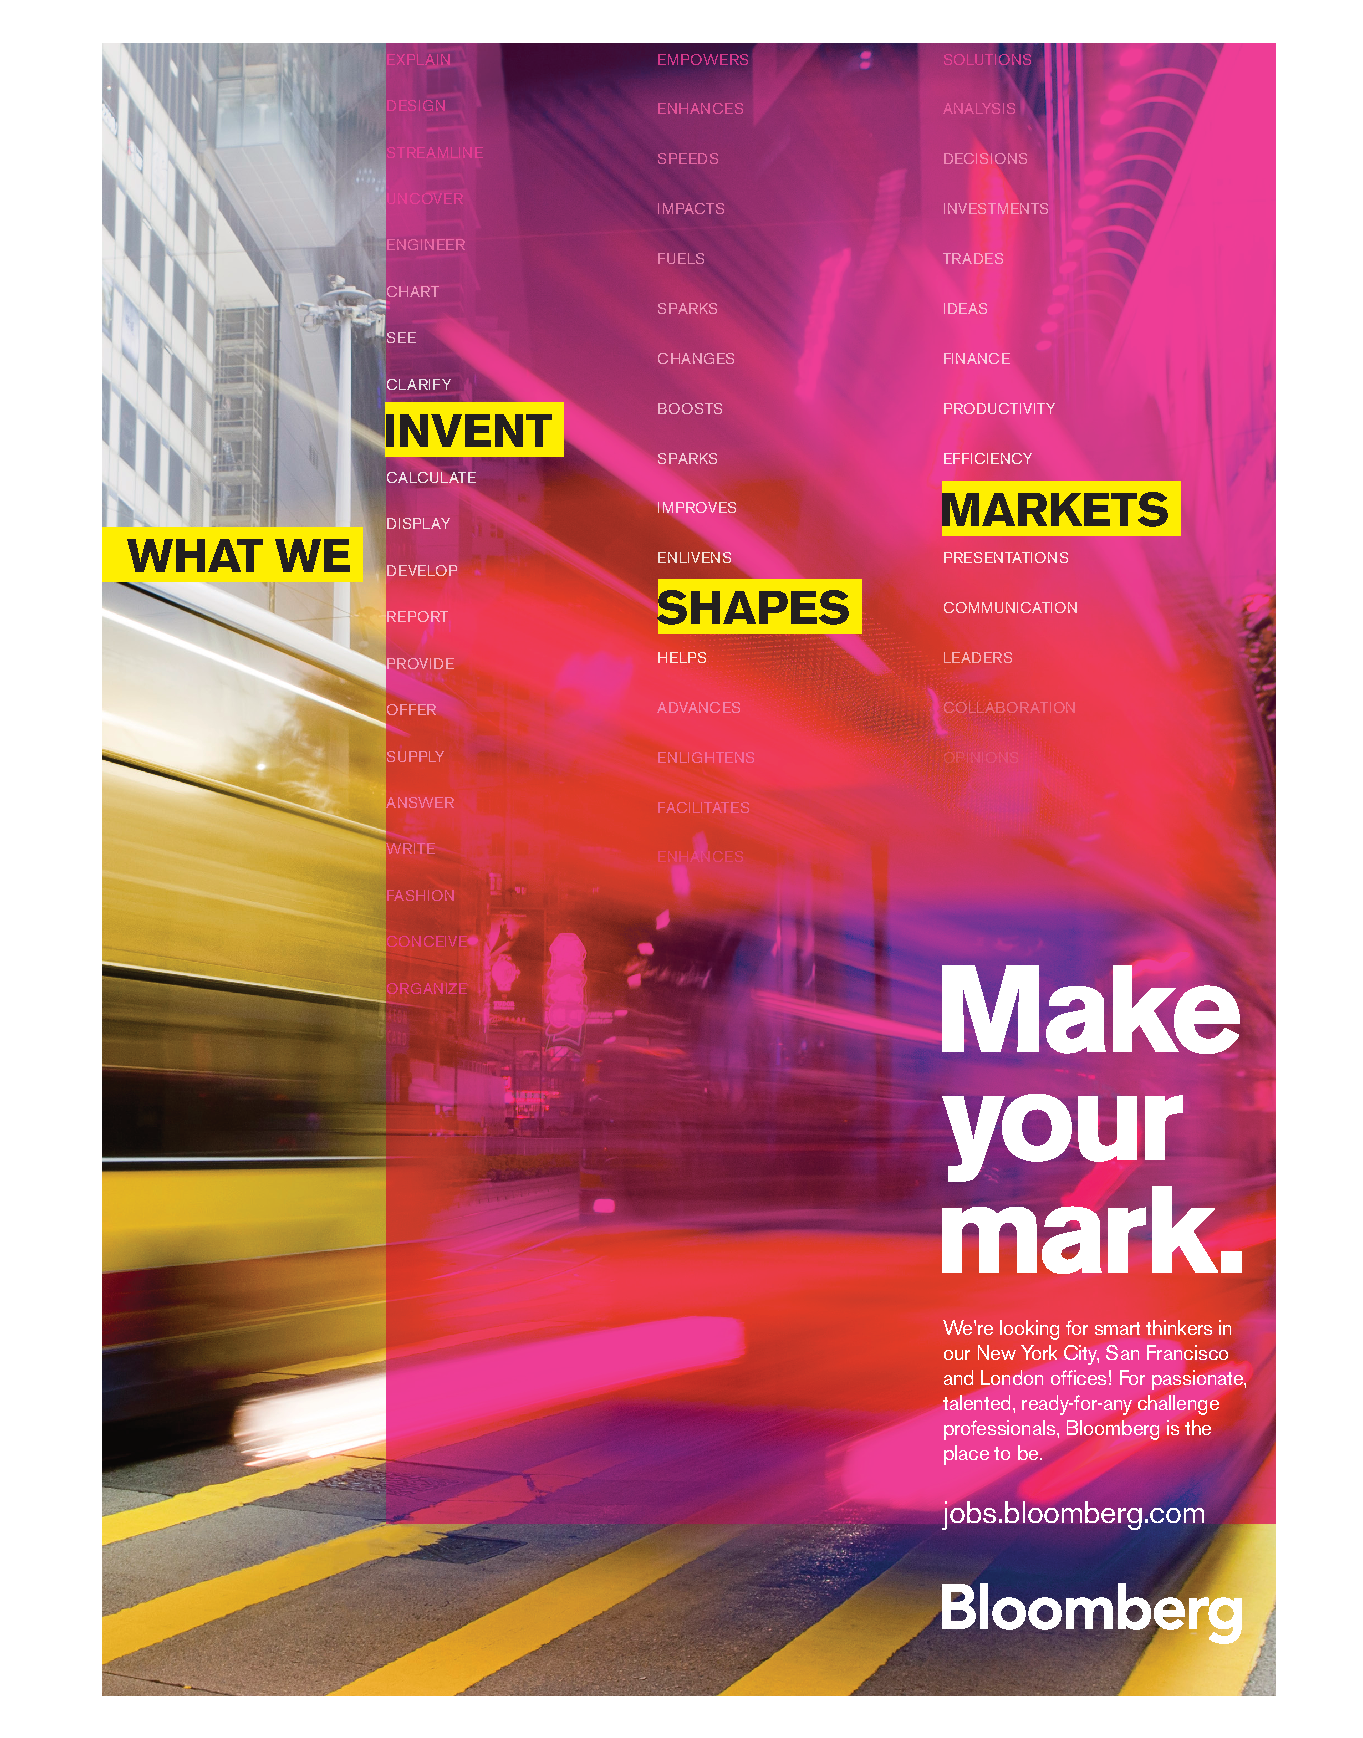
\includegraphics[width=1\textwidth]{content/images/ads/bloomberg}
\par\end{center}

\begin{center}
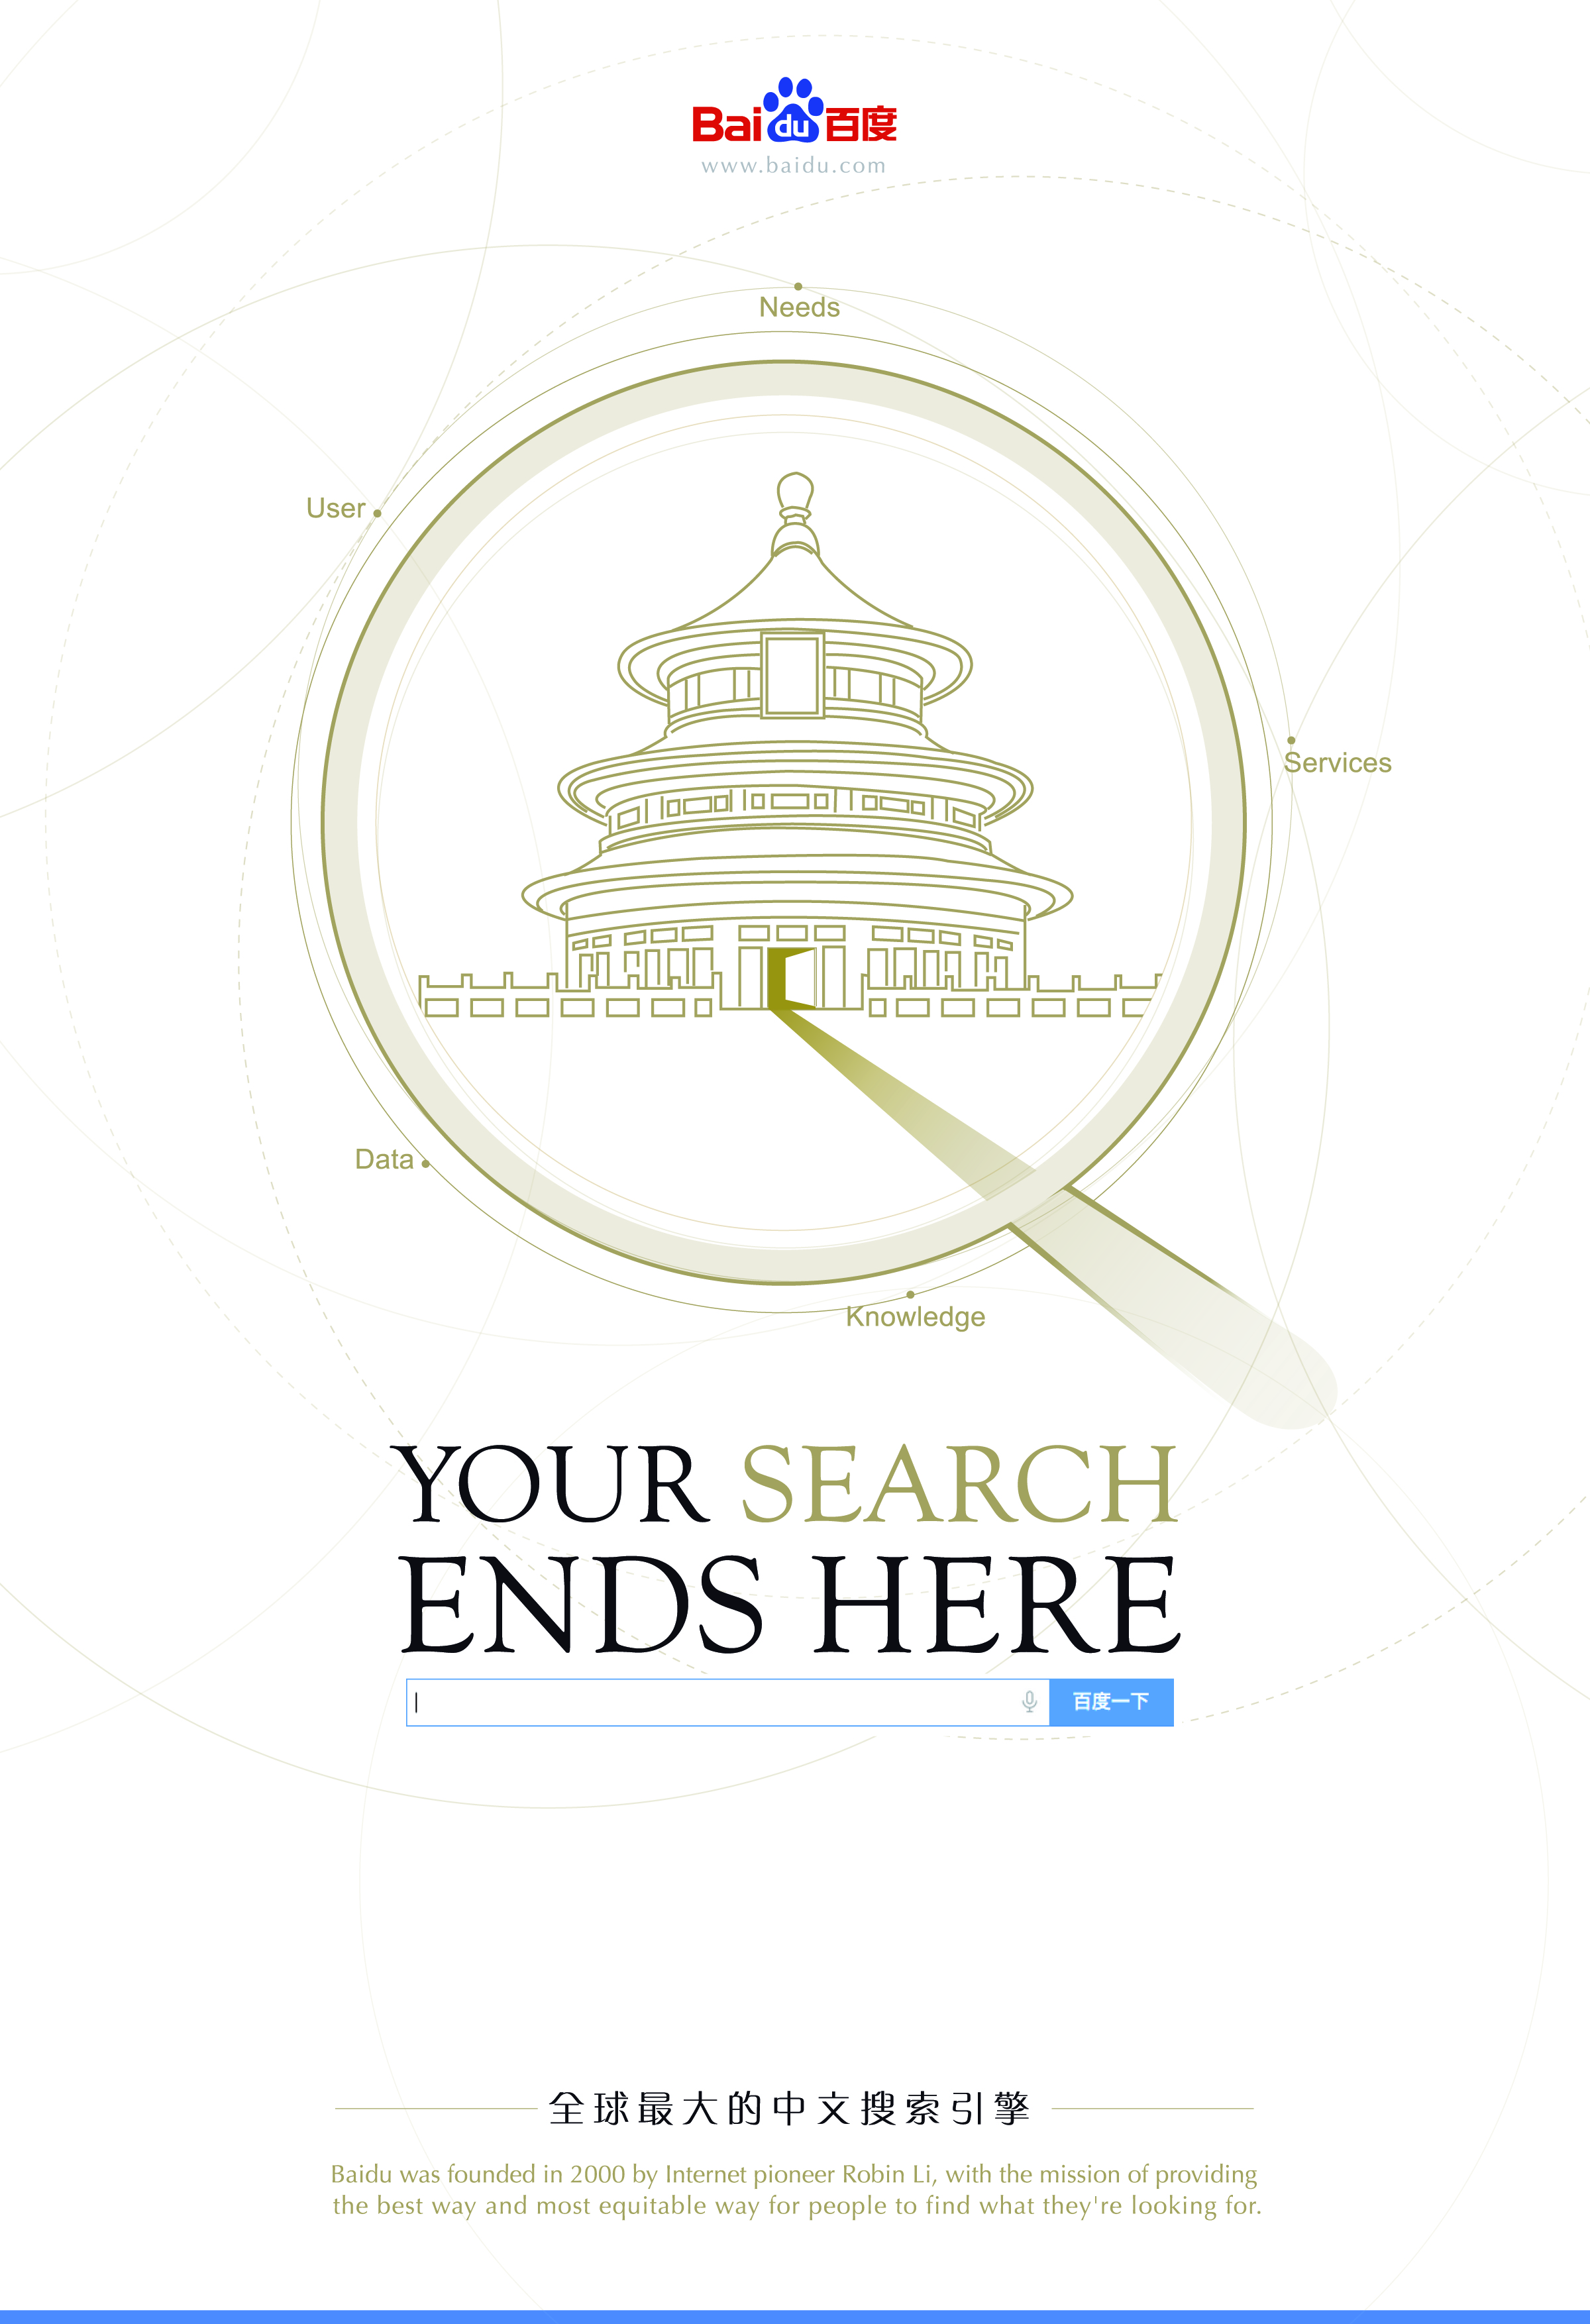
\includegraphics[width=1\textwidth]{content/images/ads/baidu}
\par\end{center}

\begin{center}
\fbox{\begin{minipage}[t][0.41\textheight][c]{0.98\columnwidth}%
\begin{center}

\includegraphics[width=0.98\textwidth]{content/images/ads/google} 
\par\end{center}%
\end{minipage}}
\par\end{center}

\begin{center}

\includegraphics[width=1\textwidth]{content/images/ads/facebook}
\par\end{center}

\begin{center}

\includegraphics[width=1\textwidth]{content/images/ads/linkedin} 
\par\end{center}

\begin{center}
\vfill{}

\par\end{center}

\begin{center}

\includegraphics[width=1\textwidth]{content/images/ads/recruit}
\par\end{center}

\vfill{}


\begin{center}

\includegraphics[width=1\textwidth]{content/images/ads/nuance}
\par\end{center}

\clearpage{}

\begin{center}
\begin{minipage}[b][1\totalheight][t]{0.48\columnwidth}%
\begin{center}

\includegraphics[width=1\textwidth]{content/images/ads/amazon}
\par\end{center}

\large

The world's brightest technology minds come to \url{Amazon.com} to
research and develop technology that improves the lives of shoppers,
sellers and developers around the world. At Amazon, our Machine Learning
team is comprised of technical leaders who develop planet-scale platforms
for machine learning on the cloud, assist in the benchmarking and
future development of existing machine learning applications across
Amazon, and help develop novel and infinitely-scalable applications.%
\end{minipage}\hfill{}
\includegraphics[width=0.48\textwidth]{content/images/ads/ai_at_isi}
\par\end{center}

\vfill{}


\begin{center}

\includegraphics[width=0.48\textwidth]{content/images/ads/voicebox}\hfill{}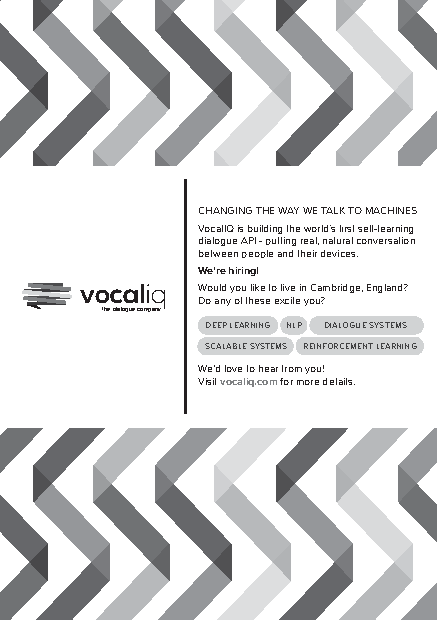
\includegraphics[width=0.48\textwidth]{content/images/ads/vocaliq}
\par\end{center}

\vfill{}


\begin{center}
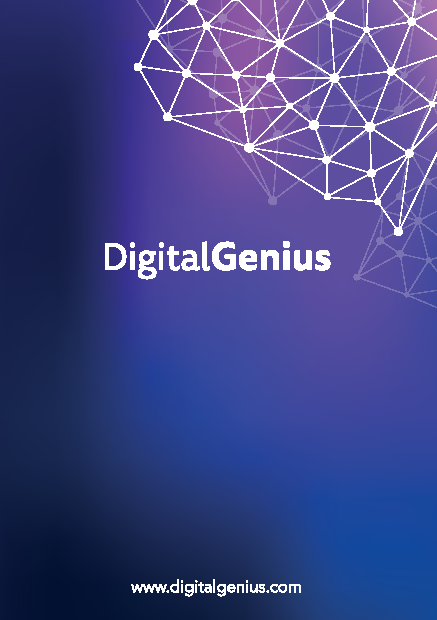
\includegraphics[width=0.48\textwidth]{content/images/ads/digitalgenius}
\par\end{center}

\begin{center}

\includegraphics[width=1\textwidth]{content/images/ads/priberam}
\par\end{center}

\vfill{}


\clearpage{}


\clearpage{}




\section*{Food Quick Reference}

\thispagestyle{fancy}
\phantomsection
\markboth{}{Food Quick Reference}
\addcontentsline{toc}{chapter}{Food Quick Reference}

A considerable number of restaurants can be found around the conference
venue. The following table shows a small selection of those restaurants
and the map that follows presents a more complete selection. \emph{Food
courts} can accomodate a large number of people and can provide a
rapid service. The closest one is the Campo Pequeno food court. Three
additional food courts are located in Saldanha, near the subway. They
are located at 15 minutes walking distance or one subway stop away
(see bottom of the map). 

\begin{center}
\begin{tabular}{cl>{\raggedright}p{0.38\columnwidth}c}
\textbf{Type} & \textbf{Establishment } & \textbf{type } & \textbf{Price }\tabularnewline
\hline 
 &  &  & \tabularnewline
\multicolumn{4}{l}{\emph{Food courts}}\tabularnewline
 & Campo Pequeno & Campo Pequeno & €\tabularnewline
 & Monumental & Praça Duque Saldanha & €\tabularnewline
 & Atrium Saldanha & Praça Duque Saldanha & €\tabularnewline
 & Saldanha Residence & Av. Fontes Pereira de Melo, 42E & €\tabularnewline
\multicolumn{4}{l}{\emph{Vegetarian and vegan}}\tabularnewline
 & Celeiro Dieta & Av. da República, 83 & €\tabularnewline
 & Paladar Zen & Av. Barbosa du Bocage, 107C & €€\tabularnewline
\multicolumn{4}{l}{\emph{Italian}}\tabularnewline
 & Italy Caffé Ristorante & Av. Duque d'Ávila, 26 & €€\tabularnewline
 & Di Casa & Avenida João XXI, 64 & €€\tabularnewline
\multicolumn{4}{l}{\emph{Indian}}\tabularnewline
 & Passage to India & Av. Praia da Vitoria, 45 & €€\tabularnewline
\multicolumn{4}{l}{\emph{Snack}}\tabularnewline
 & Padaria Portuguesa & Av. Duque de d'Ávila, 24 & €\tabularnewline
\multicolumn{4}{l}{\emph{Portuguese} }\tabularnewline
 & À Parte & Av. Defensores de Chaves, 14C & €€\tabularnewline
 & Vilhena & Rua Dona Filipa de Vilhena, 18 & €€\tabularnewline
 & Charrua do Lavrador & Av. Duque d'Ávila 13 & €€\tabularnewline
\multicolumn{4}{l}{\emph{Japanese}}\tabularnewline
 & Mayumi & Av. António José de Almeida 5C & €€\tabularnewline
 & King Sushi & Av. 5 de Outubro, 124 & €€\tabularnewline
\multicolumn{4}{l}{\emph{Fast food}}\tabularnewline
 & McDonald’s & Av. Da República, 10F & €\tabularnewline
 & McDonald’s & Av. de Roma, 3 & €\tabularnewline
\end{tabular}
\par\end{center}

\noindent \begin{center}
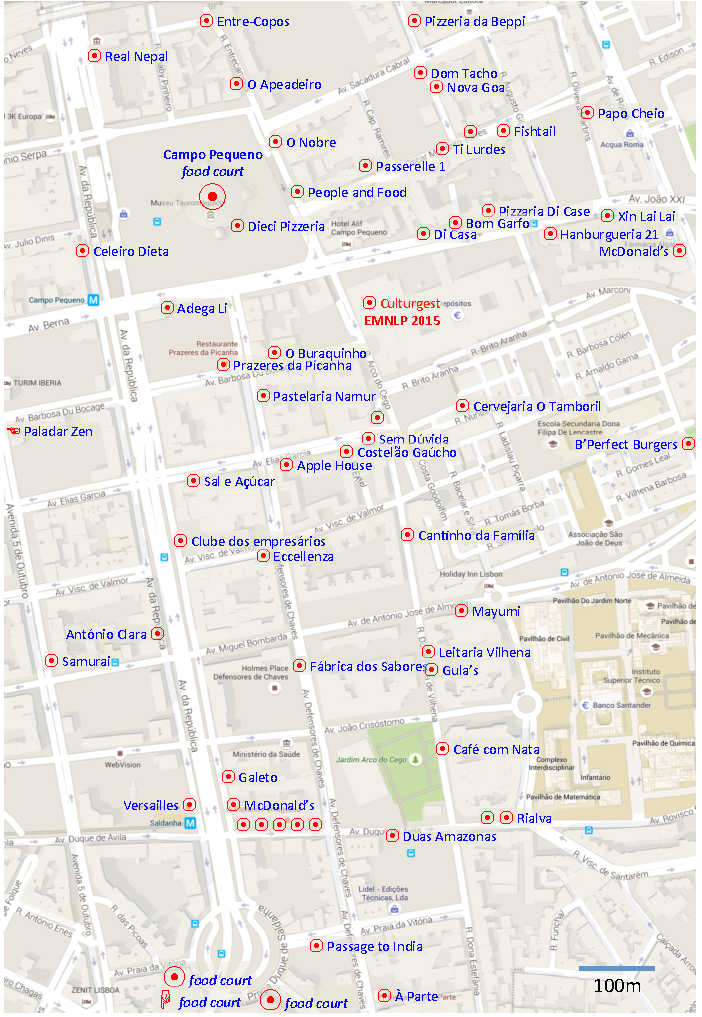
\includegraphics[width=1\columnwidth]{content/images/map-nearby-restaurants}
\par\end{center}

\noindent \thispagestyle{empty}

\noindent EMNLP 2015 gratefully acknowledges the following sponsors
for their support:\\


\noindent Platinum

\begin{center}
\quad{}\raisebox{-.6em}{
\includegraphics[width=0.45\textwidth]{content/images/logos/bloomberg}}\hfill{}
\includegraphics[width=0.45\textwidth]{content/images/logos/baidu}
\par\end{center}

\vfill{}


\noindent Gold

\begin{center}
\quad{}\raisebox{-.7em}{
\includegraphics[width=0.28\textwidth]{content/images/logos/google}}\hfill{}\raisebox{.2em}{
\includegraphics[width=0.31\textwidth]{content/images/logos/facebook}}\hfill{}
\includegraphics[width=0.32\textwidth]{content/images/logos/linkedin}
\par\end{center}

\vfill{}


\noindent Silver

\begin{center}
\quad{}\raisebox{-.7em}{
\includegraphics[width=0.3\textwidth]{content/images/logos/recruit}}\hfill{}
\includegraphics[width=0.3\textwidth]{content/images/logos/nuance}\hfill{}\raisebox{-.7em}{
\includegraphics[width=0.27\textwidth]{content/images/logos/amazon}}
\par\end{center}

\begin{center}
\quad{}\raisebox{.1em}{
\includegraphics[width=0.3\textwidth]{content/images/logos/ai_at_isi}}\hfill{}\raisebox{.3em}{
\includegraphics[width=0.3\textwidth]{content/images/logos/voicebox}}\hfill{}
\includegraphics[width=0.3\textwidth]{content/images/logos/digitalgenius}
\par\end{center}

\vfill{}


\noindent Bronze\hfill{}Best Student Paper

\begin{center}
\quad{}
\includegraphics[width=0.3\textwidth]{content/images/logos/priberam}\hfill{}\raisebox{-.3em}{
\includegraphics[width=0.3\textwidth]{content/images/logos/vocaliq}}\hfill{}\raisebox{.7em}{
\includegraphics[width=0.3\textwidth]{content/images/logos/IBMWatson}}
\par\end{center}

\vfill{}


\noindent 

\noindent Supporters

\begin{center}
\quad{}
\includegraphics[width=0.25\textwidth]{content/images/logos/rakuten-www}\hfill{}\raisebox{.7em}{
\includegraphics[width=0.25\textwidth]{content/images/logos/unbabel-www}}\hfill{}
\includegraphics[width=0.25\textwidth]{content/images/logos/cml-www}\hfill{}
\includegraphics[height=0.06\textheight]{content/images/logos/turismo-lisboa-www}
\par\end{center}

\vfill{}


\noindent Institutional partners\hfill{}Official airline

\begin{center}
\quad{}\raisebox{.7em}{
\includegraphics[width=0.2\textwidth]{content/images/logos/inesc_id-www}}\hfill{}
\includegraphics[width=0.2\textwidth]{content/images/logos/ist-www}\hfill{}
\includegraphics[width=0.25\textwidth]{content/images/logos/it-www}\hfill{}
\includegraphics[width=0.25\textwidth]{content/images/logos/tap-www}
\par\end{center}

\end{document}
